%  A simple AAU report template.
%  2015-05-08 v. 1.2.0
%  Copyright 2010-2015 by Jesper Kjær Nielsen <jkn@es.aau.dk>
%
%  This is free software: you can redistribute it and/or modify
%  it under the terms of the GNU General Public License as published by
%  the Free Software Foundation, either version 3 of the License, or
%  (at your option) any later version.
%
%  This is distributed in the hope that it will be useful,
%  but WITHOUT ANY WARRANTY; without even the implied warranty of
%  MERCHANTABILITY or FITNESS FOR A PARTICULAR PURPOSE.  See the
%  GNU General Public License for more details.
%
%  You can find the GNU General Public License at <http://www.gnu.org/licenses/>.
%
%  A simple AAU report template.
%  2015-05-08 v. 1.2.0
%  Copyright 2010-2015 by Jesper Kjær Nielsen <jkn@es.aau.dk>
%
%  This is free software: you can redistribute it and/or modify
%  it under the terms of the GNU General Public License as published by
%  the Free Software Foundation, either version 3 of the License, or
%  (at your option) any later version.
%
%  This is distributed in the hope that it will be useful,
%  but WITHOUT ANY WARRANTY; without even the implied warranty of
%  MERCHANTABILITY or FITNESS FOR A PARTICULAR PURPOSE.  See the
%  GNU General Public License for more details.
%
%  You can find the GNU General Public License at <http://www.gnu.org/licenses/>.
%
\documentclass[11pt,twoside,a4paper,openright]{report}
%%%%%%%%%%%%%%%%%%%%%%%%%%%%%%%%%%%%%%%%%%%%%%%%
% Language, Encoding and Fonts
% http://en.wikibooks.org/wiki/LaTeX/Internationalization
%%%%%%%%%%%%%%%%%%%%%%%%%%%%%%%%%%%%%%%%%%%%%%%%
% Select encoding of your inputs. Depends on
% your operating system and its default input
% encoding. Typically, you should use
%   Linux  : utf8 (most modern Linux distributions)
%            latin1 
%   Windows: ansinew
%            latin1 (works in most cases)
%   Mac    : applemac
% Notice that you can manually change the input
% encoding of your files by selecting "save as"
% an select the desired input encoding. 
\usepackage[utf8]{inputenc}
% Make latex understand and use the typographic
% rules of the language used in the document.
\usepackage[english]{babel}
%\addto\captionsenglish{\renewcommand{\chaptername}{Kapitel}}
%\addto\captionsenglish{\renewcommand{\contentsname}{Indhold}}
%\addto\captionsenglish{\renewcommand{\prefacename}{Titelblad}}
%\addto\captionsenglish{\renewcommand{\figurename}{Figur}}
%\addto\captionsenglish{\renewcommand{\tablename}{Tabel}}
%\addto\captionsenglish{\renewcommand{\appendixname}{Appendiks}}
% Use the palatino font
\usepackage[sc]{mathpazo}
\linespread{1.05}         % Palatino needs more leading (space between lines)
% Choose the font encoding
\usepackage[T1]{fontenc}
\newcommand{\hashsharp}{$^\#$}
%%%%%%%%%%%%%%%%%%%%%%%%%%%%%%%%%%%%%%%%%%%%%%%%
% Graphics and Tables
% http://en.wikibooks.org/wiki/LaTeX/Importing_Graphics
% http://en.wikibooks.org/wiki/LaTeX/Tables
% http://en.wikibooks.org/wiki/LaTeX/Colors
%%%%%%%%%%%%%%%%%%%%%%%%%%%%%%%%%%%%%%%%%%%%%%%%
% load a colour package
\usepackage{xcolor}
\definecolor{aaublue}{RGB}{33,26,82}% dark blue
\definecolor{gray}{RGB}{200,200,200} %light gray
% The standard graphics inclusion package
\usepackage{graphicx}
% Set up how figure and table captions are displayed
\usepackage{caption}
\usepackage{subcaption}
\captionsetup{%
  font=footnotesize,% set font size to footnotesize
  labelfont=bf % bold label (e.g., Figure 3.2) font
}
% Make the standard latex tables look so much better
\usepackage{array,booktabs}
% Enable the use of frames around, e.g., theorems
% The framed package is used in the example environment
\usepackage{framed}
\usepackage{float}
\usepackage{enumitem} % Enumerate with different types of counters

%%%%%%%%%%%%%%%%%%%%%%%%%%%%%%%%%%%%%%%%%%%%%%%%
% Mathematics
% http://en.wikibooks.org/wiki/LaTeX/Mathematics
%%%%%%%%%%%%%%%%%%%%%%%%%%%%%%%%%%%%%%%%%%%%%%%%
% Defines new environments such as equation,
% align and split 
\usepackage{amsmath}
% Adds new math symbols
\usepackage{amssymb}
\usepackage[makeroom]{cancel}
% Use theorems in your document
% The ntheorem package is also used for the example environment
% When using thmmarks, amsmath must be an option as well. Otherwise \eqref doesn't work anymore.
\usepackage[framed,amsmath,thmmarks]{ntheorem}
\newtheorem{theorem}{Theorem}[section]
\newtheorem{definition}{Definition}[section]
\newtheorem{lemma}{Lemma}[section]
\newtheorem{corollary}{Corollary}[section]
\theorembodyfont{\normalfont}
\newtheorem*{remark}{Remark}[chapter]
\theoremsymbol{\ensuremath{\color{black}\blacksquare}}
\newtheorem*{proof}{Proof}[section]


%%%%%%%%%%%%%%%%%%%%%%%%%%%%%%%%%%%%%%%%%%%%%%%%
% Page Layout
% http://en.wikibooks.org/wiki/LaTeX/Page_Layout
%%%%%%%%%%%%%%%%%%%%%%%%%%%%%%%%%%%%%%%%%%%%%%%%
% Change margins, papersize, etc of the document
%\usepackage[pdftex]{graphicx}
\usepackage[
  inner=28mm,% left margin on an odd page
  outer=41mm,% right margin on an odd page
  ]{geometry}
% Modify how \chapter, \section, etc. look
% The titlesec package is very configureable
\usepackage{titlesec, color}
\definecolor{gray75}{gray}{0.75}
\newcommand{\hsp}{\hspace{15pt}}
\titleformat{\chapter}[hang]{\Huge\bfseries}{\thechapter\hsp\textcolor{gray75}{\huge{|}}\hsp}{0pt}{\Huge\bfseries}
\titleclass{\part}{top}
\titleclass{\chapter}{straight}
\titleformat*{\section}{\normalfont\Large\bfseries}
\titleformat*{\subsection}{\normalfont\large\bfseries}
\titleformat*{\subsubsection}{\normalfont\normalsize\bfseries}


%\titleformat*{\paragraph}{\normalfont\normalsize\bfseries}
%\titleformat*{\subparagraph}{\normalfont\normalsize\bfseries}

%Clear empty pages between chapters
\let\origdoublepage\cleardoublepage
\newcommand{\clearemptydoublepage}{%
  \clearpage
  {\pagestyle{empty}\origdoublepage}%
}
\let\cleardoublepage\clearemptydoublepage

% Change the headers and footers
\usepackage{fancyhdr}
\pagestyle{fancy}
\fancyhf{} %delete everything
\renewcommand{\headrulewidth}{0pt} %remove the horizontal line in the header
\fancyhead[RE]{\small\nouppercase\leftmark} %even page - chapter title
\fancyhead[LO]{\small\nouppercase\rightmark} %uneven page - section title
\fancyfoot[LO,RE]{\thepage} %page number on all pages
% Do not stretch the content of a page. Instead,
% insert white space at the bottom of the page
\raggedbottom
% Enable arithmetics with length. Useful when
% typesetting the layout.
\usepackage{calc}

%%%%%%%%%%%%%%%%%%%%%%%%%%%%%%%%%%%%%%%%%%%%%%%%
% Bibliography
% http://en.wikibooks.org/wiki/LaTeX/Bibliography_Management
%%%%%%%%%%%%%%%%%%%%%%%%%%%%%%%%%%%%%%%%%%%%%%%%
\usepackage[backend=bibtex,
  bibencoding=utf8,
  sorting = nty, 
  ]{biblatex}

\addbibresource{bib/mybib}
\DeclareNameAlias{sortname}{last-first}
\DeclareNameAlias{default}{last-first}
\DefineBibliographyStrings{english}{%
  bibliography = {Bibliography},
}	
\renewcommand*{\bibfont}{\small}

%%%%%%%%%%%%%%%%%%%%%%%%%%%%%%%%%%%%%%%%%%%%%%%%
% Misc
%%%%%%%%%%%%%%%%%%%%%%%%%%%%%%%%%%%%%%%%%%%%%%%%
% Add bibliography and index to the table of
% contents
\setlength{\parindent}{0in}
\setcounter{tocdepth}{1}
\setcounter{secnumdepth}{2}
\usepackage[nottoc]{tocbibind}
% Add the command \pageref{LastPage} which refers to the
% page number of the last page
\usepackage{lastpage}
\usepackage{epstopdf}
% Add todo notes in the margin of the document
\usepackage[
  %disable, %turn off todonotes
  colorinlistoftodos, %enable a coloured square in the list of todos
  textwidth=\marginparwidth, %set the width of the todonotes
  textsize=scriptsize, %size of the text in the todonotes
  ]{todonotes}
\newcommand{\frede}[1]{\todo[color=red!40]{#1}}
\newcommand{\martin}[1]{\todo[color=green!40]{#1}}
\newcommand{\trine}[1]{\todo[color=blue!40]{#1}}
\newcommand{\chr}[1]{\todo[color=orange!40]{#1}}

%%%%%%%%%%%%%%%%%%%%%%%%%%%%%%%%%%%%%%%%%%%%%%%%
% Hyperlinks
% http://en.wikibooks.org/wiki/LaTeX/Hyperlinks
%%%%%%%%%%%%%%%%%%%%%%%%%%%%%%%%%%%%%%%%%%%%%%%%
% Enable hyperlinks and insert info into the pdf
% file. Hypperref should be loaded as one of the 
% last packages
\usepackage{hyperref}
\usepackage{url}
\hypersetup{%
	pdfpagelabels=true,%
	plainpages=false,%
	pdfauthor={Author(s)},%
	pdftitle={Title},%
	pdfsubject={Subject},%
	bookmarksnumbered=true,%
	colorlinks=false,%
	citecolor=black,%
	filecolor=black,%
	linkcolor=black,% you should probably change this to black before printing
	urlcolor=black,%
	pdfstartview=FitH%
}
%%%%%%%%%%%%%%%%%%%%%%%%%%%%%%%%%%%%%%%%%%%%%%%
\usepackage{pdfpages}	

\usepackage{todonotes}
\usepackage{listings} 
\usepackage{tikz}
\usepackage{pgfplots}
\usetikzlibrary{shapes,arrows}
\usetikzlibrary{decorations.pathreplacing}
\usetikzlibrary{calc}
\usetikzlibrary{decorations.text}

\usepackage{lmodern}
\usepackage{textcomp}
\usepackage{MnSymbol,wasysym}

%Tikz setup
\tikzset{%
  block/.style    = {draw, thick, rectangle, minimum height = 3em,
    minimum width = 3em},
  sum/.style      = {draw, circle, node distance = 2cm}, % Adder
  input/.style    = {coordinate}, % Input
  output/.style   = {coordinate} % Output
}% package inclusion and set up of the document
% see, e.g., http://en.wikibooks.org/wiki/LaTeX/Formatting#Hyphenation
% for more information on word hyphenation
\hyphenation{ex-am-ple hy-phen-a-tion short}
\hyphenation{long la-tex}
\hyphenation{ak-ti-vi-tets-track-er-ne}
\hyphenation{in-kor-po-re-re-de}
\hyphenation{com-pu-ter-en}
\hyphenation{hand-ler}
\hyphenation{be-gynd-el-ses-vist}
\hyphenation{stu-de-ren-de}
\hyphenation{mo-ti-ve-ren-de}
\hyphenation{pro-jekt-grup-pens}
\hyphenation{mål-grup-pe-a-na-ly-se}
\hyphenation{o-ver-ens}
\hyphenation{re-spon-dent-er-ne}
\hyphenation{pe-dal-fre-kvens}
\hyphenation{dif-fe-ren-tia-tion}
\hyphenation{sy-stem-er}
\hyphenation{na-bo-punkt-er}
\hyphenation{in-ter-po-la-ti-ons-e-gen-skab}
\hyphenation{sy-stem-et}
\hyphenation{pro-jekt-et}
\hyphenation{da-ta-be-hand-ling}
\hyphenation{da-ta-be-hand-ling-en}
\hyphenation{ac-ce-le-ro-me-ter}
\hyphenation{ac-ce-le-ro-me-ter-da-ta}
\hyphenation{kom-po-nent}
\hyphenation{kom-po-nent-ens}
\hyphenation{ud-sving-ning-er}
\hyphenation{be-reg-ning}
\hyphenation{Green-wich-Me-ri-di-an-en}
\hyphenation{Ind-led-nings-vist}
\hyphenation{fi-gur-er}
\hyphenation{mi-nut-tet}
\hyphenation{tids-rum}
\hyphenation{in-ter-po-la-tion}
\hyphenation{in-ter-po-la-tions-e-gen-skab}
\hyphenation{Lag-ran-ge-po-ly-no-mi-um}
\hyphenation{Lag-ran-ge-po-ly-no-mi-er}
\hyphenation{Lag-ran-ge---po-ly-no-mi-er-ne}
\hyphenation{po-ly-no-mi-um}
\hyphenation{Lag-ran-ge-po-ly-no-mi-er-ne}
\hyphenation{po-ly-no-mi-er-ne}
\hyphenation{e-ner-gi}
\hyphenation{e-ner-gi-for-brug}
\hyphenation{e-ner-gi-for-brug-et}
\hyphenation{knu-de-punkt-er}
\hyphenation{pro-blem-stil-ling}
\hyphenation{ac-ce-le-ra-tion}
\hyphenation{ac-ce-le-ra-tion-en}
\hyphenation{ac-ce-le-ra-tions-data}
\hyphenation{be-gyn-de}
\hyphenation{be-gyn-dte}
\hyphenation{ek-stra-po-le-re}
\hyphenation{ek-stra-po-le-re-de}
\hyphenation{for-ven-te}
\hyphenation{for-ven-te-de}
\hyphenation{be-skrev-et}
\hyphenation{cyk-list-er-ne}
\hyphenation{cyk-list-er}
\hyphenation{kraft-på-virk-ning}
\hyphenation{kon-klu-de-re}
\hyphenation{kon-klu-de-res}
\hyphenation{na-vi-ga-tions-sa-tel-lit-ter}
\hyphenation{be-hand-le-de}
\hyphenation{da-ta-punkt-er}
\hyphenation{mi-ni-me-res}
\hyphenation{ka-me-ra}
\hyphenation{ka-me-ra-et}
\hyphenation{ka-me-ra-op-ta-gel-se}
\hyphenation{ka-me-ra-op-ta-gel-sen}
\hyphenation{der-imod}
\hyphenation{der-ud-over}
\hyphenation{kon-ti-nu-ert}
\hyphenation{på-gæl-den-de}
\hyphenation{samp-ling}
\hyphenation{Lag-ran-ge-in-ter-po-la-tion}
\hyphenation{Lag-ran-ge-po-ly-no-mi-er-ne}
\hyphenation{om-kring}
\hyphenation{ha-stig-hed}
\hyphenation{ha-stig-hed-er}
\hyphenation{ha-stig-hed-en}
\hyphenation{lit-te-ra-tur-stu-die}
\hyphenation{nu-me-riske}
\hyphenation{til-stræk-ke-ligt}
\hyphenation{til-go-de-ser}
\hyphenation{o-ver-ve-je}
\hyphenation{o-ver-ve-jes}
\hyphenation{stu-de-ren-de}
\hyphenation{spør-ge-ske-ma}
\hyphenation{e-va-lu-e-re}
\hyphenation{pro-blem-stil-ling-en}
\hyphenation{op-ti-me-ring}
\hyphenation{op-ti-me-rings-mo-del}
\hyphenation{op-ti-me-rings-mo-del-len}
\hyphenation{punkt}
\hyphenation{punkt-er}
\hyphenation{kor-ri-ge-re}
\hyphenation{ind-led-en-de}
\hyphenation{hin-an-den}
\hyphenation{kreds-løb-et}
\hyphenation{på-be-gyn-de}
\hyphenation{på-be-gyndt}
\hyphenation{fejl-kil-de}
\hyphenation{ind-gå}
\hyphenation{ind-går}
\hyphenation{samp-le}
\hyphenation{samp-ler}
\hyphenation{samp-le-de}
\hyphenation{mi-ni-malt}
\hyphenation{ka-den-ce}
\hyphenation{a-na-ly-se}
\hyphenation{ind-be-fat-ter}
\hyphenation{funk-tion}
\hyphenation{funk-tion-en}
\hyphenation{kor-te}
\hyphenation{be-væ-gel-se}
\hyphenation{gen-tag-en-de}
\hyphenation{funk-tio-na-li-tet}
\hyphenation{for-søgs-per-son-en}
\hyphenation{mo-del}
\hyphenation{mo-del-len}
\hyphenation{pe-dal}
\hyphenation{pe-dal-en}
\hyphenation{nøj-ag-tig}
\hyphenation{løs-ning-en}
\hyphenation{INS-mo-dul-et}
\hyphenation{tekst-fil}
\hyphenation{tekst-fil-en}
\hyphenation{tekst-fil-er}
\hyphenation{tekst-fil-er-ne}
\hyphenation{an-den-grads-po-ly-no-mi-um}
\hyphenation{me-to-de}
\hyphenation{me-to-der-ne}
\hyphenation{ac-ce-le-ra-tions-må-ling}
\hyphenation{ac-ce-le-ra-tions-må-ling-en}
\hyphenation{ac-ce-le-ra-tions-må-ling-er}
\hyphenation{ac-ce-le-ra-tions-må-ling-er-ne}
\hyphenation{ud-dy-be}
\hyphenation{om-hand-ler}
\hyphenation{skibs-trans-port}
\hyphenation{ma-te-ma-ti-ske}
\hyphenation{in-ho-mo-ge-ne-ous}
\hyphenation{in-ver-ti-ble}
\hyphenation{li-ne-a-ri-se-re-de}
\hyphenation{li-ne-a-ri-se-ring-ens}
\hyphenation{eg-en-vær-di-spek-trum}
\hyphenation{o-ver-sving}
\hyphenation{und-er-dæm-pet}
\hyphenation{end-e-punkt-dif-fe-rens-en}
\hyphenation{li-ne-a-ri-se-ring}
\hyphenation{over-ens-stem-mel-sen}
\hyphenation{over-ens-stem-mel-se}
\hyphenation{en-de-punkts-dif-fe-rens}
\hyphenation{fejl-led-et}
\hyphenation{fejl-led}
\hyphenation{be-reg-nings-tid}
\hyphenation{sving-nings-tid}
\hyphenation{kon-ver-gens}
\hyphenation{kon-ver-ge-rer}
\hyphenation{pla-ce-ring}
\hyphenation{lig-nings-re-fe-ren-cer}
\hyphenation{fur-ther}
\hyphenation{o-pe-rer-es}
\hyphenation{kon-fi-gu-rer-es}
\hyphenation{dif-fe-ren-ti-al-lig-ning-er}
\hyphenation{sy-stem-er}
\hyphenation{sy-stem-pa-ra-me-tre}
\hyphenation{o-pe-rer-es}
\hyphenation{o-pe-ra-ting}
\hyphenation{sy-stem}
\hyphenation{con-ti-nu-ous}
\hyphenation{ge-ne-ra-li-zed}
\hyphenation{se-cond}
\hyphenation{mo-del-ler}
\hyphenation{lig-ning-sy-stem-et}
\hyphenation{be-gynd-el-ses-be-ting-el-ser}
\hyphenation{nær-hed-en}
\hyphenation{re-gu-la-tor-en}
\hyphenation{u-de-luk-ken-de}
\hyphenation{sta-bi-li-se-re}
\hyphenation{sy-stem-ets}
\hyphenation{re-gu-le-rer}
\hyphenation{be-gynd-el-ses-be-ting-el-ser-ne}
\hyphenation{pro-blem-stil-ling-er}
\hyphenation{an-vend-el-se}
\hyphenation{stab-len}
\hyphenation{li-ge-vægts-punkt-er}
\hyphenation{ud-sving}
\hyphenation{vir-ke-lig-hed-en}
\hyphenation{dif-fe-ren-ti-al-lig-ning-en}
\hyphenation{li-ge-vægts-punkt}
\hyphenation{li-ge-vægts-punkt-et}
\hyphenation{brug-es}
\hyphenation{be-greb}
\hyphenation{be-greb-er}
\hyphenation{kraft-en}
\hyphenation{snor-kraft}
\hyphenation{snor-kraft-en}
\hyphenation{bliv-er}%
%  A simple AAU report template.
%  2015-05-08 v. 1.2.0
%  Copyright 2010-2015 by Jesper Kjær Nielsen <jkn@es.aau.dk>
%
%  This is free software: you can redistribute it and/or modify
%  it under the terms of the GNU General Public License as published by
%  the Free Software Foundation, either version 3 of the License, or
%  (at your option) any later version.
%
%  This is distributed in the hope that it will be useful,
%  but WITHOUT ANY WARRANTY; without even the implied warranty of
%  MERCHANTABILITY or FITNESS FOR A PARTICULAR PURPOSE.  See the
%  GNU General Public License for more details.
%
%  You can find the GNU General Public License at <http://www.gnu.org/licenses/>.
%
%
%
% see, e.g., http://en.wikibooks.org/wiki/LaTeX/Customizing_LaTeX#New_commands
% for more information on how to create macros

%%%%%%%%%%%%%%%%%%%%%%%%%%%%%%%%%%%%%%%%%%%%%%%%
% Macros for the titlepage
%%%%%%%%%%%%%%%%%%%%%%%%%%%%%%%%%%%%%%%%%%%%%%%%
%Creates the aau titlepage
\newcommand{\aautitlepage}[3]{%
  {
    %set up various length
    \ifx\titlepageleftcolumnwidth\undefined
      \newlength{\titlepageleftcolumnwidth}
      \newlength{\titlepagerightcolumnwidth}
    \fi
    \setlength{\titlepageleftcolumnwidth}{0.5\textwidth-\tabcolsep}
    \setlength{\titlepagerightcolumnwidth}{\textwidth-2\tabcolsep-\titlepageleftcolumnwidth}
    %create title page
    \thispagestyle{empty}
    \noindent%
    \begin{tabular}{@{}ll@{}}
      \parbox{\titlepageleftcolumnwidth}{
        \iflanguage{danish}{%
          
\includegraphics[width=\titlepageleftcolumnwidth]{figures/aau_logo_da}
        }{%
          
\includegraphics[width=\titlepageleftcolumnwidth]{figures/aau_logo_en}
        }
      } &
      \parbox{\titlepagerightcolumnwidth}{\raggedleft\sf\small
        #2
      }\bigskip\\
       #1 &
      \parbox[t]{\titlepagerightcolumnwidth}{%
      \textbf{Synopsis:}\bigskip\par
        \fbox{\parbox{\titlepagerightcolumnwidth-2\fboxsep-2\fboxrule}{%
          #3
        }}
      }\\
    \end{tabular}
    \vfill
    \iflanguage{danish}{%
      \noindent{\footnotesize\emph{Rapportens indhold er frit tilgængeligt, men offentliggørelse (med kildeangivelse) må kun ske efter aftale med forfatterne.}}
    }{%
      \noindent{\footnotesize\emph{The content of this report is freely available, but publication (with reference) may only be pursued due to agreement with the author.}}
    }
    \clearpage
  }
}

%Create english project info
\newcommand{\englishprojectinfo}[8]{%
  \parbox[t]{\titlepageleftcolumnwidth}{
    \textbf{Title:}\\ #1\bigskip\par
    \textbf{Theme:}\\ #2\bigskip\par
    \textbf{Project Period:}\\ #3\bigskip\par
    \textbf{Project Group:}\\ #4\bigskip\par
    \textbf{Participant(s):}\\ #5\bigskip\par
    \textbf{Supervisor(s):}\\ #6\bigskip\par
    \textbf{Copies:} #7\bigskip\par
    \textbf{Page Numbers:} \pageref{LastPage}\bigskip\par
    \textbf{Date of Completion:}\\ #8
  }
}

%Create danish project info
\newcommand{\danishprojectinfo}[8]{%
  \parbox[t]{\titlepageleftcolumnwidth}{
    \textbf{Titel:}\\ #1\bigskip\par
    \textbf{Tema:}\\ #2\bigskip\par
    \textbf{Projektperiode:}\\ #3\bigskip\par
    \textbf{Projektgruppe:}\\ #4\bigskip\par
    \textbf{Deltagere:}\\ #5\bigskip\par
    \textbf{Vejledere:}\\ #6\bigskip\par
    \textbf{Oplagstal:} #7\bigskip\par
    \textbf{Sidetal:} \pageref{LastPage}\bigskip\par
    \textbf{Afleveringsdato:}\\ #8
  }
}

%%%%%%%%%%%%%%%%%%%%%%%%%%%%%%%%%%%%%%%%%%%%%%%%
% An example environment
%%%%%%%%%%%%%%%%%%%%%%%%%%%%%%%%%%%%%%%%%%%%%%%%
\theoremheaderfont{\normalfont\bfseries}
\theorembodyfont{\normalfont}
\theoremstyle{break}
\def\theoremframecommand{{\color{gray!50}\vrule width 5pt \hspace{5pt}}}
\newshadedtheorem{exa}{Example}[chapter]
\newenvironment{example}[1]{%
		\begin{exa}[#1]
}{%
		\end{exa}
}
% my new macros
\begin{document}
%frontmatter
\pagestyle{empty} %disable headers and footers
\pagenumbering{roman} %use roman page numbering in the frontmatter
%\lstset{
%	language = C,
%	backgroundcolor=\color{gray},
%	basicstyle=\ttfamily,
%	keywordstyle=\color{red},
%	numberstyle=\tiny\color{black},
%	numbers = left,
%	numbersep=5pt,
%	captionpos=b
%	}
%\def\inline{\lstinline[basicstyle=\ttfamily,keywordstyle={}]}

%  A simple AAU report template.
%  2015-05-08 v. 1.2.0
%  Copyright 2010-2015 by Jesper Kjær Nielsen <jkn@es.aau.dk>
%
%  This is free software: you can redistribute it and/or modify
%  it under the terms of the GNU General Public License as published by
%  the Free Software Foundation, either version 3 of the License, or
%  (at your option) any later version.
%
%  This is distributed in the hope that it will be useful,
%  but WITHOUT ANY WARRANTY; without even the implied warranty of
%  MERCHANTABILITY or FITNESS FOR A PARTICULAR PURPOSE.  See the
%  GNU General Public License for more details.
%
%  You can find the GNU General Public License at <http://www.gnu.org/licenses/>.
%
\pdfbookmark[0]{Front page}{label:frontpage}%
\begin{titlepage}
  \addtolength{\hoffset}{0.5\evensidemargin-0.5\oddsidemargin} %set equal margins on the frontpage - remove this line if you want default margins
  \noindent%
  \begin{tabular}{@{}p{\textwidth}@{}}
    \toprule[2pt]
    \midrule
    \vspace{0.2cm}
    \begin{center}
    \Huge{\textbf{
      Signals and systems
    }}
    \end{center}
    \begin{center}
      \Large{
        Time and frequency analysis of music signals % insert your subtitle here
      }
    \end{center}
    \vspace{0.2cm}\\
    \midrule
    \toprule[2pt]
  \end{tabular}
 % \vspace{4 cm}
  \begin{center}
    {\large
      Project report
    }\\
    \vspace{0.2cm}
    {\Large
      Mattek4 G4-101a
    }
  \end{center}

%indsæt figur

\begin{figure}[H]
\centering
\hspace*{-2cm}
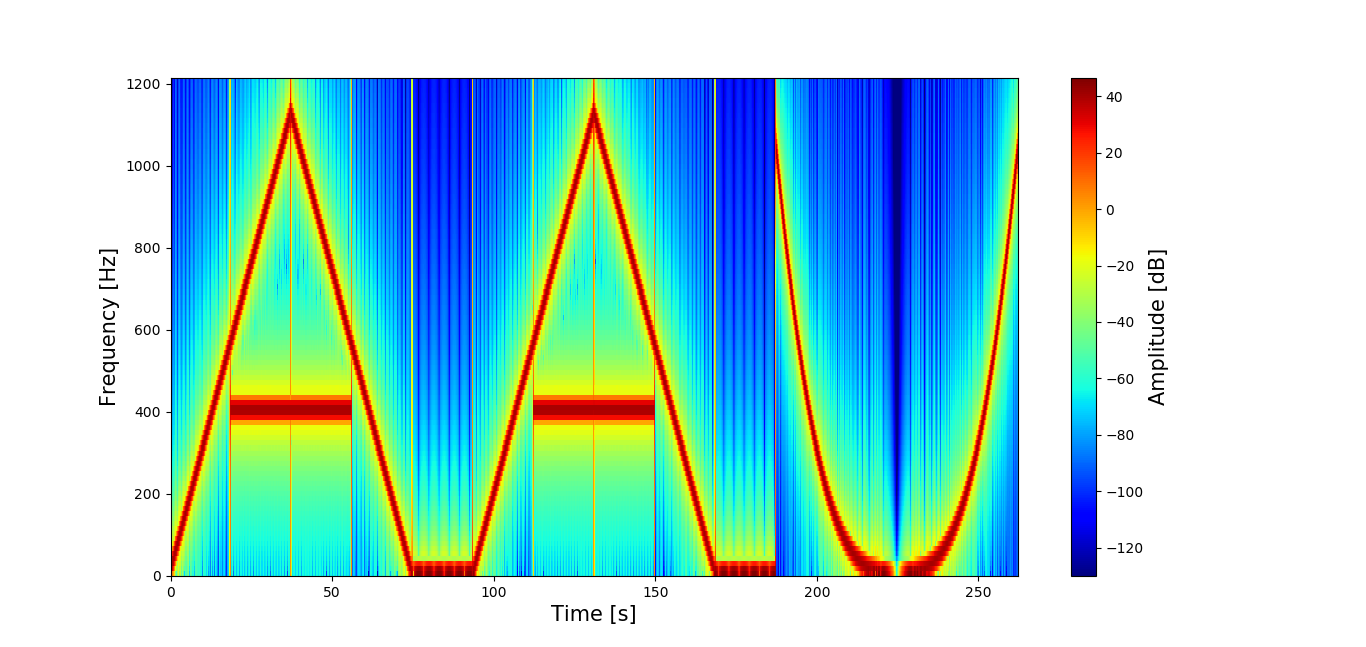
\includegraphics[width=1.4\textwidth]{figures/aaulogo.png}
\end{figure}

  %\vfill
  \begin{center}
  Aalborg University\\
  Department of Mathematical Sciences
  \end{center}
\end{titlepage}
\clearpage

\thispagestyle{empty}
{\small
\strut\vfill % push the content to the bottom of the page
\noindent Copyright \copyright{} Aalborg University 2016\par
\vspace{0.2cm}
\noindent In this project Python 2.7.11 has been applied for data processing and to draw graphs. The project is written in \LaTeX.
% \noindent I dette projekt er Python 2.7.11 anvendt til databehandling understøttet af matplotlib.pyplot til at opstille grafer. Projektet er skrevet i \LaTeX.
\clearpage


%\pdfbookmark[0]{English title page}{label:titlepage_en}
%\aautitlepage{%
%  \englishprojectinfo{
%    Project Title %title
%  }{%
%    Scientific Theme %theme
%  }{%
%    Fall Semester 2010 %project period
%  }{%
%    XXX % project group
%  }{%
%    %list of group members
%    Author 1\\ 
%    Author 2\\
%    Author 3
%  }{%
%    %list of supervisors
%    Supervisor 1\\
%    Supervisor 2
%  }{%
%    1 % number of printed copies
%  }{%
%    \today % date of completion
%  }%
%}{%department and address
%  \textbf{Electronics and IT}\\
%  Aalborg University\\
%  \href{http://www.aau.dk}{http://www.aau.dk}
%}{% the abstract
%  Here is the abstract
%}

\cleardoublepage
{\selectlanguage{danish}
\pdfbookmark[0]{Titelside}{label:titlepage_da}
\aautitlepage{%
  \danishprojectinfo{
    Tid- og frekvensanalyse af musik-signaler
  }{%
	Signaler og systemer
  }{%
    Forårssemester 2017%project period
  }{%
	Mattek4 G4-101
  }{%
    Trine Nyholm Jensen \\
  }{%
    Athanasios Georgiadis \\
    Jakob Stoustrup
  }{%
    6 % number of printed copies
  }{%
	19. december 2016
  }%
}{%department and address
  \textbf{Matematik-Teknologi}\\
  Aalborg Universitet\\
  \href{http://www.aau.dk}{http://www.aau.dk}
}{% the abstract
indsæt }
}
\cleardoublepage
\pdfbookmark[0]{Table of Contents}{label:contents}
\pagestyle{fancy} %enable headers and footers again
\tableofcontents

\listoftodos	
\clearpage
\chapter*{Preface}
\addcontentsline{toc}{chapter}
{Preface}
Indsæt forord!
\\
\vspace{\baselineskip}\hfill Aalborg University, \today
\vfill\noindent
\begin{minipage}[b]{0.45\textwidth}
 \centering
 \rule{\textwidth}{0.5pt}\\
Christian Hilligsøe Toft\\
 {\footnotesize \href{mailto:cht15@student.aau.dk}{cht15@student.aau.dk}}  
\end{minipage}
\hfill
\begin{minipage}[b]{0.45\textwidth}
 \centering
 \rule{\textwidth}{0.5pt}\\
Frederik Appel Vardinghus-Nielsen\\
 {\footnotesize \href{mailto:fvardi15@student.aau.dk}{fvardi15@student.aau.dk}}
\end{minipage}
\vspace{3\baselineskip}
\vspace{1\baselineskip}
\begin{minipage}[b]{0.45\textwidth}
 \centering
 \rule{\textwidth}{0.5pt}\\
Martin Kamp Dalgaard\\
 {\footnotesize \href{mailto:mkda15@student.aau.dk}{mkda15@student.aau.dk}}  
\end{minipage}
\hfill
\begin{minipage}[b]{0.45\textwidth}
 \centering
 \rule{\textwidth}{0.5pt}\\
 Trine Nyholm Jensen\\
 {\footnotesize \href{mailto:trijen15@student.aau.dk}{trijen15@student.aau.dk}}  
\end{minipage}
\vspace{2\baselineskip}
\vspace{1\baselineskip}
\cleardoublepage
%mainmatter
\pagenumbering{arabic} %use arabic page numbering in the mainmatter
\chapter{Problem analysis} \label{ch1}
In this chapter an introduction will lead to a discussion of problems encountered by a musician when music is to be transcribed. The importance of these problems is analysed and the need for a solution assessed whereafter existing and possible solutions with roots in mathematics will be presented. The chapter will conclude with a \textit{problem statement} which will form the basis for the rest of the project.
\section{Introduction}
Some musicians are capable of playing without reading music written on a sheet of music, and they invent new music through a creative process where they play by ear and do not have the need to write down their compositions. Creative thinking and processes are however interruptable and this can be problematic when the need for transcribing a composition - so as to remember or convey it to others - to a sheet of music arises. This may ruin the creative proces by exactly interrupting it because one needs to concentrate on the transcription.\\\\
To ease the creative process of a musician it is imaginable that some kind of automatic real time transcription of musical compositions can be developed which will eliminate the problem of having to interrupt the aforementioned process.
\section{Problem analysis}
Although the first system of musical notation is the Sumerian system created 3,500 years ago music has existed for much longer. \cite{origins} This means that people have been playing music without any form of written music until then. Even with the creation of standardised musical notation musicianship on high level is possible without any form of education and/or skills in reading and writing music. As such there continue to exist musicians without aforementioned skills.\\\\
Inability to read or write music poses no problem in itself, as it doesn't necessarily hinder musical creativity. Problems however arise when the need to convey or remember musical compositions presents itself. Just as standardised languages make everyday communication and tasks easier a standardised musical notation is needed to convey compositions to others without anyone having to remember the compositions in their entirety. Standard musical notation has been created but has to be learned and research suggests that the ability to read and write music varies considerably from person to person and might even be affected by dyslexia. \cite{dyslexia} In short people are genetically diverse when it comes to learning to read music.\\\\
If musical transcription in the middle of a creative process potentially interrupts said process the effect would be increasingly strengthened by the inability to quickly perform transcriptions which in the worst case scenario would require another person to do the transcription. These consequences of the inability to read/write in musical notation may hinder the distribution of otherwise ingenious musical creations.
\subsection{Existing and possible solutions}
There has been undertaken plenty of research regarding automatic transcription of music and the material is to find in both books \cite{sol1} and articles \cite{sol2}. There also exists downloadable software which helps transcription by hand \cite{transcribe!}. The extensive research done stems from the applications extending to other areas than just transcribing music for musicians - making computers participate with human performances is another imaginable application. Although the research is extensive "[$\hdots$]the performance of transcription systems is still significantly below that of a human expert[$\hdots$]" \cite{future} and so there is room for improvement.\\\\
This project will focus on creating a solution with the use of the mathematical tools of harmonic analysis with the Fourier Transform and of digital filtering to exstract signal information from a digitalized analog signal. The focus will furthermore be on the limitations for this project and the methods used and how these might be overcome. The viability of an algorithm based on the mathematical tools will be tested in a lab to further illustrate the possibilities and limitations of said algorithm. \todo{Her skal måske uddybes, når vi ved mere om vores løsning og metode}
\subsection{Problem statement}
The above analysis is summarized.\\
When musicians compose new music they firstly play but it stunts their creativity when they need to stop to transcribe the music. There is furthermore not necessarily any correlation between musical talent and the ability to transcribe music. This makes it advantageous for many musicians to use a program which automatically transcribes music to a sheet of music. This leads to the following problem statement:
\begin{itemize}
\item[] \textit{How can an algorithm through the use of mathematical tools be designed to automatically transcribe music to a spectrogram?}
\end{itemize}
\section{Limitations}
This project will be limited to focusing on the learning process in designing an algorithm capable of recognizing sound frequencies and translating them to a spectrogram. The spectrogram will furthermore not be a musical score, as this requires complicated algorithms for the recognition of different notes. Instead the spectrogram will show the continuum of frequencies along one axis.\\\\
The music used for testing the algorithm will be simple melodies comtaining one note at a time (no chords) from one instrument at a time. This will allow insight into the methods used without complicating the recognition of notes by blending together different instruments and different sound frequencies.\\\\
The music transcription will be done in non-real time - the designed algorithm will be used on a prerecorded piece of music. This makes it possible to run the algorithm without having to play the piece of music every time and furthermore makes it possible to neglect computational power and/or efficiency.\\\\
As such the end product of this project will ideally be limited to being an algorithm based on mathematical tools which is capable of transcribing a prerecorded piece of simple music to a spectregram. 
%\input{sections/mainmatter/chapter_1/_____.tex}

\cleardoublepage
\chapter{Overskrift} \label{ch2}

\chapter{Musikteori}
I dette kapitel introduceres grundlæggende musikteori, der anvendes i projektet.
\\ \\
I nodesystemet er en node en symbolsk repræsentation af en bestemt tone, som er tilknyttet en specifik frekvens (angivet i hertz, Hz). Hver node indeholder således information om tonens højde og desuden også om dens varighed. Et nodeark er således en symbolsk repræsentation af et diagram over tid og frekvens, hvilket også kaldes et spektrogram.
\\ \\
Til at notere noder benytter man et nodesystem, der består af fem vandrette linjer, hvor noderne er placeret. Grundlæggende findes der 12 forskellige toner Noderne i nodesystemet består først og fremmest af stamtoner, som navngives med bogstaverne A-G afhængigt af deres vertikale placering. Efter G starter navngivningen forfra med det næste A, der ligger en oktav over det forrige. Mellem flere af stamtonerne ligger andre toner, som sammen med stamtonerne udgør de 12 grundtoner, som typisk anvendes i musik. Afstanden mellem alle grundtonerne er en halv tone.

Eksempler på nodernes placeringer fremgår af figur \ref{Cdur}, der er en såkaldt C-dur angivet i G-nøglen. At det er en C-dur betyder, at den starter ved C, går op til G og videre over A, B og til slut C, der ligger en oktav over C. At noderne er angivet i G-nøglen ses ved symbolet i starten af nodesystemet. Der findes mange forskellige nøgler i musik, og G-nøglen angiver, at den nederste tone på figur \ref{Cdur} er det såkaldte nøglehuls-C (der på gamle klaverer ligger ud for nøglehullet), og at A'et mellem den anden- og tredje nederste linje er kammertonen. Kammertonen vælges som definition normalt til at være 440 Hz, men kan dog svinge med $pm 3 Hz$ afhængigt af den enkelte musiker eller orkester, der spiller musikken. Samtlige andre toner i 

\begin{figure}[H]
    \centering
    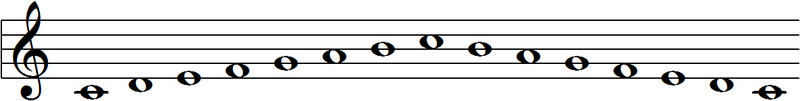
\includegraphics[width = 0.6\textwidth]{figures/C_dur.PNG}
    \caption{C-dur.}
    \label{Cdur}
\end{figure}

I dette projekt betragtes nodesystemet gennem G-nøglen





\cleardoublepage
\chapter{Frekvensanalyse}
I dette kapitel foretages der frekvensanalyse af det samplede signal $s[n]$. Dette gøres for at undersøge signalets frekvensmæssige indhold og fortsætte det videre arbejde med modifikation af signalets indhold.

\section{Dokumentation af algoritmer}
Frekvensanalysen gøres mulig med den diskrete Fouriertransformation (DFT), som beregnes ved hjælp af en \textit{fast Fourier transform}-algoritme (FFT) baseret på Cooley-Tukey algoritmen. Algoritmen er implementeret i Python og udnytter DFT-summens symmetri til at lave en rekursiv opdeling af summen, således den beregningsmæssige kompleksitet nedbringes fra $O(N^2)$ (naiv implementering af DFT) til $O(N\log N)$ for store $N$, hvor $N$ er datalængden. Herunder ses implementeringen af DFT og FFT i et Pythonscript.
\begin{lstlisting}
def DFT(x,c):
    X = np.zeros(c,dtype=complex)
    for k in range(len(x)):
        a = 0+0*1j
        for n in range(c):
            a += x[n]*np.exp(-2*np.pi*1j*k*n/float(c))
            X[k] = a
    return X

def is_power2(num): # Checks if a number is a power of 2
	return num != 0 and ((num & (num - 1)) == 0)

def FFT(x):
    N_new = len(x)
    if is_power2(N_new) == False:
        raise ValueError("N skal vaere en potens af 2.")
    elif N_new == 2:
        return DFT(x,N_new) # Returnerer DFT naar data ikke kan deles mere op
    else:
        X_even = FFT(x[::2]) # Deler rekursivt input op - lige dele
        X_odd = FFT(x[1::2]) # Deler rekursivt input op - ulige dele
        factor = np.exp(-2j * np.pi * np.arange(N_new) / N_new) # Twiddlefaktor
        return np.concatenate([X_even + factor[:int(N_new / 2)] * X_odd,
                               X_even + factor[int(N_new / 2):] * X_odd])
\end{lstlisting}

\section{Tids- og frekvensplot}
I dette afsnit undersøges signalets frekvensspektrum og hvordan dette afhænger af antallet af samples $N$ og samplingsfrekvensen $f_s$. Det vides, at opløsningen i tid afhænger af $f_s$ og at opløsningen i frekvens afhænger af $f_s$ og $N$, således
\begin{align} \label{eq:tidsoploesning}
T = \frac{1}{f_s}\phantom{m}\text{og}\phantom{m} bin=\frac{f_s}{N},
\end{align}

hvor $T$ er samplingsperioden og $bin$ er intervallet mellem to diskrete frekvenser i frekvensdomænet. Dette afsnit undersøger disse relationer.\\
På figur \ref{fig:1} ses signalet i tids- og frekvensdomænet samplet med $f_s=1$ Hz og med $N=2^8, 2^{12}, 2^{18}$ samples.

\begin{figure}[H]
\begin{minipage}{0.49\textwidth}
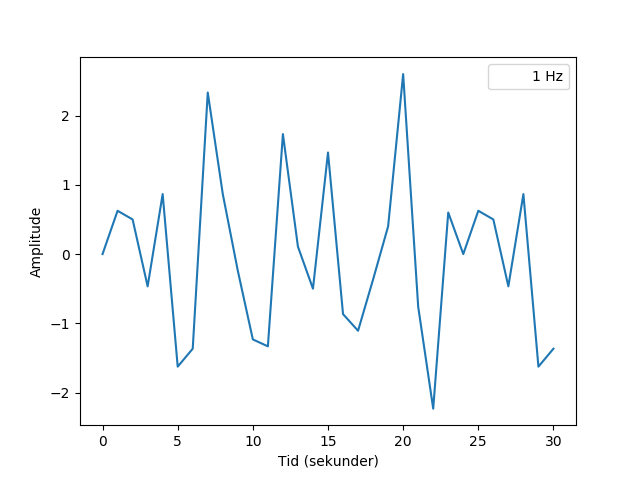
\includegraphics[width=\textwidth]{figures/signal_1hz.png}
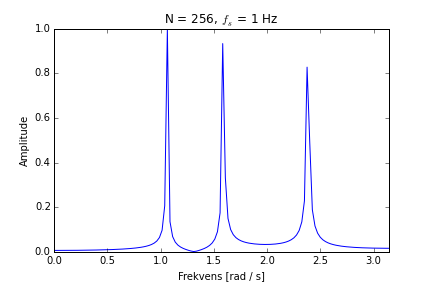
\includegraphics[width=\textwidth]{figures/frekvensanalyse/freq_1hz_N256}
\end{minipage}
\begin{minipage}{0.49\textwidth}
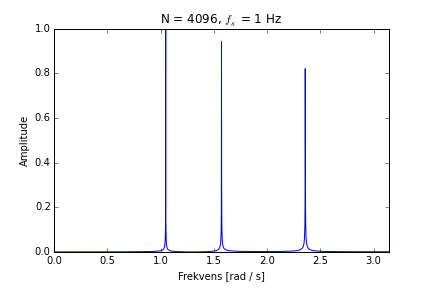
\includegraphics[width=\textwidth]{figures/frekvensanalyse/freq_1hz_N4096.png}
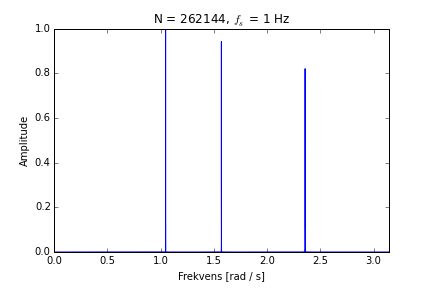
\includegraphics[width=\textwidth]{figures/frekvensanalyse/freq_1hz_N262144.png}
\end{minipage}
\caption{Plot af signal samplet ved $f_s=1$ Hz i tidsdomænet og plot af de tilhørende frekvensdomæner for antal af samples $N = 2^8, 2^{12}, 2^{18}$.}
\label{fig:1}
\end{figure}

På figur \ref{fig:2} ses signalet ligeledes i tids- og frekvensdomænet samplet med $f_s=32$ Hz og med $N=2^8, 2^{12}, 2^{18}$ samples.

\begin{figure}[H]
\begin{minipage}{0.49\textwidth}
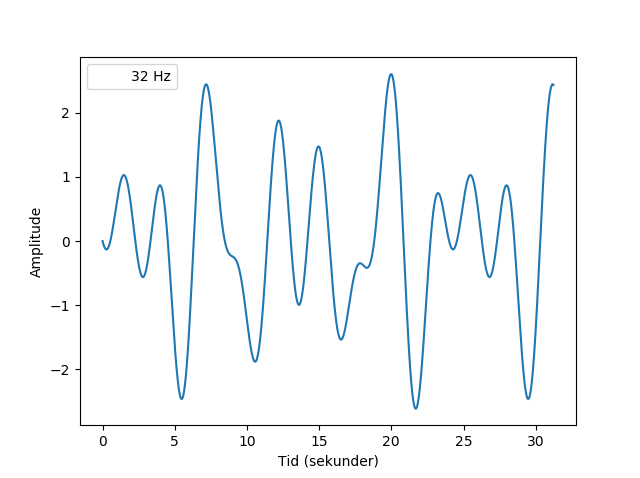
\includegraphics[width=\textwidth]{figures/signal_32hz.png}
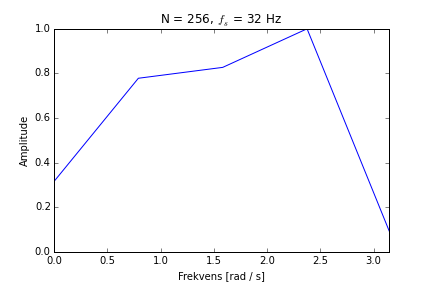
\includegraphics[width=\textwidth]{figures/frekvensanalyse/freq_32hz_N256}
\end{minipage}
\begin{minipage}{0.49\textwidth}
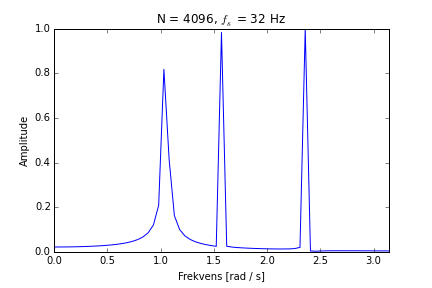
\includegraphics[width=\textwidth]{figures/frekvensanalyse/freq_32hz_N4096.png}
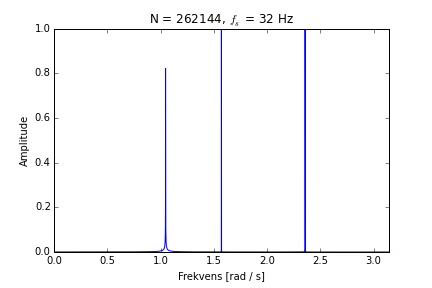
\includegraphics[width=\textwidth]{figures/frekvensanalyse/freq_32hz_N262144.png}
\end{minipage}
\caption{Plot af signal samplet ved $f_s=32$ Hz i tidsdomænet og plot af udsnit af de tilhørende frekvensdomæner for antal af samples $N=2^8, 2^{12}, 2^{18}$.}
\label{fig:2}
\end{figure}

\section{Diskussion}
Det ses tydeligt på tidsdomænerne i figur \ref{fig:1} og figur \ref{fig:2}, at opløsningen af signalet i tid afhænger af $f_s$ og bliver bedre som $f_s$ stiger. Dette stemmer overens med \eqref{eq:tidsoploesning}.
\\ \\
Det ses ligeledes tydeligt, at opløsningen i frekvensdomænet afhænger af $N$ og bliver bedre som $N$ stiger. Det er ydermere bemærkelsesværdigt, at øgning af $f_s$ giver ringere opløsning i frekvensdomænet som set i andet plot i figur \ref{fig:2}. Disse observationer stemmer ligeledes overens med \eqref{eq:tidsoploesning}.
\\ \\
Det ses i figur \ref{fig:1} og \ref{fig:2}, at amplituderne for de tre frekvenser, som signalet indeholder, ikke er lige store, selvom signalet tydeligvis er konstrueret således. Det ses også på figur \ref{fig:1} og figur \ref{fig:2}, at amplituderne varierer som $f_s$ varierer, men ikke som $N$ varierer. Dette skyldes spektral lækage, og er ikke et problem for rekonstruktion af signalet, da energien blot er distribueret rundt om den frekvens, som den bør forefindes ved, således amplituden bliver 1.

%\section{Delkonklusion}
%Frekvensanalysen af signalet afslørede tydeligt de tre frekvenser, som optræder i signalet, og det blev vist, hvordan opløsningen af signalet i tid og frekvens afhænger af $f_s$ og $N$ - bedre opløsning i tid betyder generelt ringere opløsning i frekvens og omvendt. At lade $N$ være arbitrært stor er ikke en mulighed, da den beregningsmæssige kompleksitet afhænger af $N$ og der ikke haves uendelig regnekraft. På baggrund af disse overvejelser skal der træffes en beslutning om fastlæggelsen af $f_s$ og $N$.
\cleardoublepage
\chapter{$\mathcal{L}^p$ and $\ell^p$ spaces} \label{ch4}

This chapter is inspired by \cite{FAA}, \cite{FSP} and \cite{FTFA}.
\\ \\
This project deals with functions in the so-called $\mathcal{L}^p$ and $\ell^p$ spaces. These spaces are introduced in the following and used later to ensure that the Fourier series and transforms used in the project actually converge. The following definitions are inspired by \cite{page 31, FSP}.

\begin{definition}{$\mathcal{L}^p(\mathbb{R})$}
\\
Let $D \subset \mathbb{R}^n$ be a subset. $\mathcal{L}^2(D)$ is the set of all functions on $D$ whose squares are absolutely Lebesgue-integrable over $D$:
\begin{align*}
\mathcal{L}^2(D) = \left\{ f: \int_D |f(x)|^2 dx < \infty \right\}
\end{align*}

$\mathcal{L}^2(D)$ is the normed vector space of square-integrable complex-valued functions. The inner product is:
\begin{align*}
\langle x,y \rangle =  \int_D x(t) \overline{y(t)} dt
\end{align*}

Where $\overline{y(t)}$ is the complex conjugate of $y(t)$. The norm is:
\begin{align*}
\|x\| = \left( \int_D |x(t)|^2 dt \right)^{1/2}
\end{align*}

This definition can be expanded for any $p \in [1,\infty)$ and all of $\mathbb{R}$ such that the normed vector space $\mathcal{L}^p(\mathbb{R})$ is the subspace of $\mathbb{C}^\mathbb{R}$ consisting of vectors with finite $\mathcal{L}^p$ norm:
\begin{align*}
\|x\|_p = \left( \int_{-\infty}^\infty |x(t)|^p dt \right)^{1/p}
\end{align*}
\end{definition}

As stated in \cite{page 74, FAA}, this space is simply the space of all functions $f$ such that the region between the graph of $|f|^2$ and the $x$-axis has finite area. The Lebesgue integral is therefore just another way of calculating the area between the graph of the function and the $x$-axis. The Lebesgue integral will not be elaborated further in this project as it is beyond its focus.
\\ \\
A similar definition is given for $\ell^p$ which deals with sequences:
\begin{definition}{$\ell^p(\mathbb{Z})$}
\\
$\ell^2(\mathbb{Z})$ is the space of square-summable sequences, and the inner product is defined as:
\begin{align*}
\langle x,y \rangle = \sum_{n\in\mathbb{Z}} x[n] \overline{y[n]}
\end{align*}

And the norm is defined as:
\begin{align*}
\|x\| = \left( \sum_{n\in\mathbb{Z}} |x[n]|^2 \right)^{1/2}
\end{align*}

For any $p \in [1,\infty)$, the normed vector space $\ell^p(\mathbb{Z})$ is the subspace of $\mathbb{C}^N$ consisting of vectors with finite $\ell^p$ norm:
\begin{align*}
\|x\|_p = \left( \sum_{n\in\mathbb{Z}} |x[n]|^p \right)^{1/p}
\end{align*}

Furthermore, the $\ell^\infty$ norm is defined as:
\begin{align*}
\|x\|_\infty = \sup_{n\in\mathbb{Z}}|x[n]|
\end{align*}
\end{definition}


Noter fra vejledermødet 28-02-2017:
\begin{align*}
\|f\|_{L^p} = \left( \int_{-\infty}^\infty |f(x)|^p dx \right)^{1/p} \\
\langle f,g \rangle = \int_{-\infty}^\infty f(x) \overline{g(x)} dx
\end{align*}
(ligesom angivet ovenfor). Hvis $f \in L^1$ eller $L^2$ og $g \in L^1$ (mindst én i $L^1$), så gælder der:
\begin{align*}
F(f*g) = \hat{f} \cdot \hat{g}
\end{align*}

Altså er foldning i tidsdomænet det samme som at gange i frekvensdomænet.

\begin{align*}
L^p(\mathbb{R}) =
\left\{\begin{matrix}
f : \mathbb{R} \to \mathbb{C}: \int_{-\infty}^\infty |f(x)|^p dx < \infty \\
Measureable (integrationsteori)
\end{matrix}\right.
\end{align*}

$$

%The following should be rewritten as it is almost copied directly from the book.
%\\ \\
%From Folland, p. 81-82:
%One can replace the element $dx$ of linear measure on $[a,b]$ by a weighted element of measure, $w(x) dx$. To be precise, suppose $w$ is a continuous function on $[a,b]$ such that $w(x) > 0$ for all $x \in [a,b]$; we call such a $w$ a weight function on $[a,b]$. We can then define the weighted $L^2$ space $L^2_w(a,b)$ to be the set of all (Lebesgue measurable) functions on $[a,b]$ such that
%\begin{align*}
%\int_a^b |f(x)|^2 w(x) dx < \infty,
%\end{align*}
%
%and we define an inner product and norm on $L_w^2(a,b)$ by
%\begin{align*}
%\langle f,g \rangle = \int_a^b f(x) \overline{g(x)} w(x) dx, \quad \|f\|_w = \left( \int_a^b |f(x)|^2 w(x) dx \right)^{1/2}
%\end{align*}
%
%We define $L_2(D)$ to be the set of all functions $f$ such that:
%\begin{align*}
%\int_D |f(\textbf{x})|^2 d\textbf{x} < \infty
%\end{align*}
%
%and we define the inner product and norm on $L^2(D)$ by
%\begin{align*}
%\langle f,g \rangle = \int_D f(\textbf{x}) \overline{g(\textbf{x})} d \textbf{x}, \quad \|f\| = \left( \int_D |f(\textbf{x})|^2 d \textbf{x} \right)^{1/2}.
%\end{align*}
%
%Another example of a Hilbert space is the space $l^2$ of square-summable sequences. That is, the elements of $l^2$ are sequences $\{c_n\}_1^\infty$ of complex numbers such that $\sum_1^\infty |c_n|^2 < \infty$, and the inner product and norm are defined by
%\begin{align*}
%\left\langle \{c_n\},\{d_n\} \right\rangle = \sum_1^\infty c_n \overline{d}_n, \quad \left\| \{c_n\} \right\| = \left( \sum_1^\infty  |c_n|^2 \right)^{1/2}
%\end{align*}
%\\ \\
%From M. Vetterli, page 35:
%$\mathcal{L}^p(\mathbb{R})$ spaces Like for sequences, we can define other norms on $\mathbb{C}^\mathbb{R}$ as well. Again, because the space is infinite-dimensional, the choice of the norm and the requirement that it be finite restricts $\mathbb{C}^\mathbb{R}$ to a smaller set. For example, for $p \in [1,\infty)$, the $\mathcal{L}^p$ norm is
%\begin{align*}
%\|x\|_p = \left( \int_{-\infty}^{\infty} |x(t)|^p dt \right)^{1/p}
%\end{align*}
%
%The extension to $p = \infty$ leads to the $\mathcal{L}^\infty$ norm as
%\begin{align*}
%\|x\|_\infty = ess \sup_{t\in\mathbb{R}} |x(t)|.
%\end{align*}


\cleardoublepage
\chapter{Fourier transforms} \label{ch5}
The following chapter will focus on different aspects on the Fourier series and the Fourier transform.

\section{Fourier series}
Functions can be represented as a linear combination of functions on the form $\sin nt$.
Or in other words linear combination of a oscillating function, sines, cosines or equivalently complex exponential.
\\\\
It can be an advantage to decompose functions, as a series or integral of "simpler" functions, to retrieve information.
\begin{align*}
	f(x) = \sum_{n=1}^\infty c_n f_n(x)\text{, or } f(x)= \int_{-\infty}^\infty g(u) h(u,x) du
\end{align*}
Information from a function $f(x)$ will, as an example be stored in the coefficient $\{c_n\}_{n=1}^\infty$.
The coefficients can easily be stored on a computer.
\\\\ 
Furthermore a function $f: \mathbb{R}\to\mathbb{R}$ (or $\mathbb{C}$) is called $2\pi$-periodic, if $f(\theta + 2\pi) = f(\theta), \forall\theta\in\mathbb{R}$

The idea of the Fourier series is using the above information to recreate a $2\pi$- periodic signal.\\
The Fourier series is defined as:
\begin{align*}
	f(t) &= a_0 + \sum_{n=1}^\infty(a_n \cos(n \omega t) + b_n \sin(n \omega t))\\
	&= \sum_{n=-\infty}^{\infty} c_n e^{n j\omega t} 
\end{align*}
The second part holds per Euler's formula:
\begin{align*}
	\cos(n(\theta) = \dfrac{e^{j n \theta} + e^{-j n \theta}}{2} \text{ and } \sin(n \theta) = \dfrac{e^{jn\theta}-e^{jn\theta}}{2j}
\end{align*}

It can be simpler to work with the complex exponential function, but working with the trigonometric functions $\cos$ and $\sin$ have there advantages. 
Like being real-valued and odd and even, for cosine and sine respectively.

\subsection{Calculation of the coefficient $c_n$}
It is a necessity to calculate the $c_n$ coefficient.
By the assumption that this can be done, and it's permissible to integrate the fourier series term by term: :\\
\\
To solve $c_n$ in the equation $f(t)= \sum_{n=-\infty}^{\infty} c_n e^{n j\omega t}$
\\\\
First multiply both sides by $e^{-(j\omega k t)}$, where $k\in \mathbb{Z}$. And integrate both sides over a given period, from $-\pi$ to $\pi$:

\begin{align} \label{eq:firststep_fouriercoefficient}
	\int_{-\pi}^\pi f(t)e^{-(j\omega k t)} = \int_{-\pi}^\pi \sum_{n=-\infty}^{\infty} c_n e^{n j\omega t} e^{-j\omega k t} dt
\end{align}
The integration of a $2\pi$ - periodic function over the length of the period, can be shifted with an integer.

\begin{lemma}\label{lemma:2pi-periodic_function}
Suppose $F$ is $2\pi$ - periodic and integrable. Then for any real number a 

\begin{align}
\int_a^{2\pi+a}F(t) dt = \int_0^{2\pi}F(t)dt
\end{align}
\end{lemma}
\begin{proof}
\begin{align*}
	\int_0^{2\pi}F(t)dt 
	&= \int_0^a F(t) dt + \int_a^{2\pi} 
	= \int_0^a F(t+2\pi)dt + \int_a^{2\pi} F(t) dt\\ 
	&= \int_{2\pi}^{2\pi + a} F(t) dt + \int_a^{2\pi}F(t)dt
	= \int_a^{2\pi}F(t)dt	+ \int_{2\pi}^{2\pi + a} F(t)dt \\
	&= \int_a^{2\pi+a}F(t)dt
\end{align*}
\end{proof}
Pulling the summation and the constant on the right-hand side out of the integral in \eqref{eq:firststep_fouriercoefficient} yields the following:
\begin{align*}
	\int_{-\pi}^\pi f(t) e^{-j \omega k t}dt
	= \sum_{-\infty}^\infty c_n \int_{\pi}^\pi e^{-j \omega(n-k)t}dt
\end{align*} 
The integral on the right-hand side has two cases to consider, $n \neq k$ and $n = k$\\\\
For $n\neq k$:
\begin{align*}
	\forall n,n\neq k: \int_{-\pi}^\pi e^{j\omega(n-k)t}dt 
	=\dfrac{1}{j\omega(n-k)}e^{j\omega(n-k)t}\mid_{-\pi}^{\pi}
	=\dfrac{(-1)^{n-k}-1(-1)^{n-k}}{j\omega(n-k)}
	=0
\end{align*}
\chr{Could be written with sine and cosine, to show that the integral of those 2 over a periode is 0}
The second case is for $n = k$
\begin{align*}
	\forall n,n=k: \int_{-\pi}^\pi e^{j\omega(n-k)t}dt = \int_{-\pi}^\pi dt = 2\pi
\end{align*}
The integral can be concluded to yield either $0$ or $2\pi$:
\begin{align}
	\int_{-\pi}^{\pi} e^{j \omega (n-k)t}dt 
	= 
	\begin{cases}
			2\pi \text{ if } n=k\\
			0 \text{ otherwise}
	\end{cases}
\end{align}
The coefficient $c_n$'s general equation is then:
\begin{align*}
	c_n = \dfrac{1}{2\pi} \int_{-\pi}^{\pi} f(t) e^{-(j \omega nt)}dt
\end{align*} 
\begin{definition} \label{def:fourier_definition}
Fourier series of a $2\pi$ - periodic integrabel function $f(t)$ is defined as:
\begin{align*}
	\sum_{n=-\infty}^\infty c_n e^{j n \omega t}
\end{align*}
where $c_n = \dfrac{1}{2\pi}\int_{- \pi}^\pi f(t) e^{-j n \omega t}$
\\\\
Alternatively:
\begin{align*}
	\dfrac{a_0}{2} + \sum_{n=1}^{\infty} \left[ a_n \cos(n \omega t) + b_n \sin(n \omega t)\right]
\end{align*} 
where
\begin{align*}
	a_n 
	&= \dfrac{1}{\pi} \int_{-\pi}^\pi f(t) \cos (n \omega t) dt, \, n=0,1,\dots\\
	b_n
	&= \dfrac{1}{\pi} \int_{-\pi}^\pi f(t) \sin (n \omega t) dt, \, n=1,2,\dots	
\end{align*}
\end{definition}
Further if a function $g(t)$ is uneven, ($g(t) = -g(-t)$), then the integral $\int_{-\pi}^\pi g(t) = 0$.
\subsection{Convergence of the Fourier series}
For a $2\pi$- periodic and integrabel function, the n'th. order Fourier partial-sum is defined by: 
\begin{align}\label{eq:partialsumFourierSeries}
	S_N^f(t) = \dfrac{1}{2} a_0 + \sum_1^N\left(a_n \cos n\omega t + b_n \sin n \omega t \right) = \sum_{-N}^N c_n e^jn\omega t
\end{align}
with the coefficients $a_n$ and $b_n$ or $c_n$ defined as in \ref{def:fourier_definition}.\\
\\
Inserting $c_n$ in the partial sum using $x$ in place of the variable $t$.
\begin{align*}
	S_N^f(t)
	= \dfrac{1}{2\pi}\sum_{-N}^N \int_{-\pi}^\pi f(x) e^{-j n \omega x} dx\, e^{jn\omega t}\\
	= \dfrac{1}{2\pi}\sum_{k = -N}^N \int_{-\pi}^\pi f(x) e^{j k \omega (x-t)} d(x)
\end{align*}
Notice that 
\begin{align*}
	S_N^f (t) 
	&= \dfrac{1}{2\pi} \sum_{n=-N}^N \int_{-\pi}^\pi f(x)e^{jn\omega(x-t)} dx\text{, and let } 
	\tau 
	= x-t\\
	&= \dfrac{1}{2\pi} \sum_{n = -N}^N \int_{-\pi - x}^{\pi - x} f(x + \tau ) e^{j n\omega \tau} d\tau
\end{align*}
By \ref{lemma:2pi-periodic_function} the above equation can be expressed as followed:
\begin{align*}
	S_N^f (\omega t) 
	&= \dfrac{1}{2\pi} \sum_{n=-N}^N \int_{-\pi}^\pi f(t + \tau) e^{jn \omega t} d\tau\\
	&= \int_{-\pi}^\pi f(t + \tau) D_N(\tau) d\tau
\end{align*}
Where $D_N = \dfrac{1}{2\pi}\sum_{n=-N}^{N}e^omega{jn\\tau}$ is a Dirichlet-core. 
The integral from $-\pi$ to $\pi$ of a Dirichlet-core is $\dfrac{1}{2}$ \chr{(Ref bogen for at undgå at snakke om Dirichlet kernen (kunne evt. vises ud fra Mortens noter)}
Using this information the follwing can be derived:
\begin{theorem}
	Let $f(t)$ be a $2\pi$-periodic and piece wise smooth then the limit of the partial sum $S_N^f$ is given by:
	 \begin{align*}
	 	\lim_{N\to\infty} S_N^f (t) = \dfrac{1}{2}\left[f(t-) + f(t+)\right], \, t\in [-\pi, \pi]
	 \end{align*}
	If $f$, is continues in $t$, then:
	\begin{align*}
		\lim_{N\to \infty} S_N^F(t) = f(t).
	\end{align*}
\end{theorem}
\begin{proof}
	\begin{align*}
	\dfrac{1}{2} f(\theta-) = f(\theta-) \int_{-\pi}^0 D_n(\tau)d\tau \text{ and } \dfrac{1}{2}f(\theta+) = f(\theta+) \int_0^\pi D_n (\tau)d\tau
	\end{align*}
	Which gives
\end{proof}
%%%%%%
More precisely, $f\in PS(a,b)$ iff 
\begin{enumerate}
	\item $f \in PC(a,b)$
	\item $f'$ exists and is continuous on $(a,b)$ except perhaps at finitely many points $x_1,\dots,x_k$ (which will include any points where f is discontinuous), and the one-sided limits $f'(x_j-)$ and $f'(x_j+)(j)1,\dots,K)$, and also $f'(a+)$ and $f'(b-)$, exist.
\end{enumerate}
The sum of any infinite series is defined to be the limit of its partial sums.
The N partial sum of the Fourier series be defined as:
\begin{align}\label{eq:partialsumFourierSeries}
	S_N^f(\omega t) = \dfrac{1}{2} a_0 + \sum_1^N\left(a_n \cos n\omega t + b_n \sin n \omega t \right) = \sum_{-N}^N c_n e^jn\omega t
\end{align}
Wants to show that the partial sum \eqref{eq:partialsumFourierSeries} converges.
Inserting the definition $a_n$ and $b_n$ or $c_n$ coefficients into \eqref{eq:partialsumFourierSeries} yields:
\begin{align*}
	S_N^f(\omega t) = \dfrac{1}{2\pi} \sum_{-N}^N \int_{-\pi}^\pi 
\end{align*}
%http://cnx.org/contents/8YnJdzjg@8/Derivation-of-Fourier-Coeffici

%Note to self foldning.

\section{The Fourier transform}
\cleardoublepage
\chapter{Sample theory} \label{ch6}
In this chapter sample theory and its importance when converting an analogue audio signal to a digital audio signal along with its complications is treated.
%\section{The frequency domain}
%The following sections look at functions in both the \textit{time}- and \textit{frequency} domains and utilizes the advantages of these different visualizations. To express a function of time as a function of frequency the \textit{Fourier transform} is used. The transform decomposes a periodic function $A$ of time $t$ into an amplitude valued function $\hat{A}$ of frequency $\omega$ and shows which amplitudes of frequencies of different sinusoids are present in the signal. The mathematical background for the Fourier transform is reserved for chapter \ref{ch5} - this chapter will make do with the graphical explanation in figures \ref{fig:time} and \ref{fig:freq}. Notice the both real and imaginary amplitudes of $\hat{A}$.
%\begin{figure}[H]
%\centering
%\begin{minipage}{0.49\textwidth}
%\centering
%\begin{tikzpicture}[scale=0.8]
%\begin{axis}[
%axis lines=middle,
%xtick={-3.14159,3.14159},
%xticklabels={$-\pi$,$\pi$},
%ytick={-1.5,1.5}
%,xmin=-4.25
%,xmax=4.25
%,ymin=-1.75
%,ymax=1.75,
%samples=50]
%\addplot[red][domain=-3.14159:3.14159] {sin(deg(x))+(1/2)*cos(deg(2*x))};
%\end{axis}
%\end{tikzpicture}
%\caption{Graph of $f(x)=\sin x + \frac{1}{2} \cos 2x$ in the time domain.}
%\label{fig:time}
%\end{minipage}
%\centering
%\begin{minipage}{0.49\textwidth}
%\centering
%\begin{tikzpicture}[scale=0.8]
%\begin{axis}[
%axis lines=middle,
%xtick={-6.28318,-3.14159,3.14159,6.28318},
%xticklabels={$-2\pi$,$-\pi$,$\pi$,$2\pi$},
%ytick={-1.5,1.5},
%xmin=-6.75,
%xmax=6.75,
%ymin=-1.75,
%ymax=1.75,]
%\draw[->][red](axis cs:6.28318,0)--(axis cs:6.28318,0.62665);
%\draw[->][red](axis cs:-6.28318,0)--(axis cs:-6.28318,0.62665);
%\draw[->][blue](axis cs:3.14159,0)--(axis cs:3.14159,1.2533);
%\draw[->][blue](axis cs:-3.14159,0)--(axis cs:-3.14159,1.2533);
%\end{axis}
%\end{tikzpicture}
%\caption{Graph of $\hat{f}$ in the frequency domain. Red = real, blue = imaginary.}
%\label{fig:freq}
%\end{minipage}
%\end{figure}
%The above figures illustrate the continuous Fourier transform. The transform can be discretized to the discrete Fourier transform, which is crucial, when working with sampled signals. This is likewise covered in chapter \ref{ch5}.
\section{Sampling}
Sampling is the process of representing a \textit{continuous-time} signal by a sequence of values. Doing so converts the continuous-time signal into a \textit{discrete-time} signal. \cite{pelgrom} The relation between a continuous function $x_c(t)$ and the discrete funtion $x[n]$ obtained by sampling $x_c(t)$ is described by
\begin{equation}\label{eq:sampling_principle}
x[n]=x_c(nT_s)
\end{equation}
where the \textit{sampling period }$T_s$ (time bewteen two consecutive samples) is determined by the \textit{sampling frequency} $f_s$ (samples pr. second). The relation between $T_s$, $f_s$ and the times of samplings is described by
\begin{equation}\label{eq:sample_freq}
t=\frac{n}{f_s}=nT_s, \phantom{mm} n=-\infty,\hdots-1,0,1\hdots,\infty \phantom{mm}\text{\cite{pelgrom}}
\end{equation}
where $n$ is the number of samples.\\\\
To describe sampling mathematically the \textit{Dirac delta} function is introduced in definition \ref{def:dirac}.
\begin{definition}[Dirac delta function]\label{def:dirac}
The Dirac delta function is the function $\delta$ satisfying
\begin{equation}
\int_{-\infty}^{\infty} \! f(t)\delta(t-t_0) \, dt=f(t_0).\phantom{mm}\text{\cite{pelgrom}}
\end{equation}
\end{definition}
Summing an infinite number of Dirac functions shifted at equally spaced time intervals $nT_s$ as in \eqref{eq:dirac_sum} produces a constant function of equidistant Dirac pulses:
\begin{equation}\label{eq:dirac_sum}
s(t)=\sum_{n=-\infty}^{\infty}\delta(t-nT_s)\phantom{mm}\text{\cite{DTSP}}
\end{equation}
Multiplying a continuous signal with \eqref{eq:dirac_sum} and using the property of the Dirac function \eqref{eq:sampling} is obtained:
\begin{align}
x_s(t)&=x_c(t)s(t)\nonumber \\
&=x_c(t)\sum_{n=-\infty}^{\infty}\delta(t - nT_s)\nonumber \\
&=\sum_{n=-\infty}^{\infty}x_c(t)\delta(t - nT_s)\nonumber\\
&=\sum_{n=-\infty}^{\infty}x_c(nT_s)\delta(t - nT_s)\phantom{mm}
\label{eq:sampling}
\end{align}
\eqref{eq:sampling} is a mathematical representation of sampling of the continuous function $x_c(t)$ into the function $x_s(t)$ \cite{DTSP}. Although \eqref{eq:sampling} describes sampling, we have $x_s(t)\neq x[n]$ as $x_s(t)$ is defined in the interval between two samples whereas $x[n]$ only takes values at integers $n$. Although $x_s(t)\neq x[n]$ \eqref{eq:sampling} will be useful in the upcoming appliance of the Fourier transform.
\paragraph{Example of sampling} Sampling a ball following the arc shown in figure \ref{fig:ball_cont} results in the plotted points in figure \ref{fig:ball_disc}. As such the balls path is illustrated with discrete points along the path.
\begin{figure}[H]
\centering
\begin{minipage}{0.49\textwidth}
\centering
\begin{tikzpicture}[scale=1.4]
\draw[->] (-0.25,0) -- (4.25,0) node[right] {$x$};
\draw[->] (0,-0.25) -- (0,2) node[above] {$y$};
\draw[scale=1,domain=0:4,smooth,variable=\x,red] plot ({\x},{-0.25*\x*\x+\x});
\end{tikzpicture}
\caption{Trajectory of a ball described by the time continuous function $x_c(t)$. In continuous time the trajectory is smooth.}
\label{fig:ball_cont}
\end{minipage}
\centering
\begin{minipage}{0.49\textwidth}
\centering
\begin{tikzpicture}[scale=1.4]
\draw[->] (-0.25,0) -- (4.25,0) node[right] {$x$};
\draw[->] (0,-0.25) -- (0,2) node[above] {$y$};
\draw(0,0) node {\textbullet};
\draw(0.5,0.4375) node {\textbullet};
\draw(1,0.75) node {\textbullet};
\draw(1.5,0.9375) node {\textbullet};
\draw(2,1) node {\textbullet};
\draw(2.5,0.9375) node {\textbullet};
\draw(3,0.75) node {\textbullet};
\draw(3.5,0.4375) node {\textbullet};
\draw(4,0) node {\textbullet};
\end{tikzpicture}
\caption{Trajectory of a ball described by the time discrete function $x[n]$. The trajectory consists of samples of $x_c(t)$.}
\label{fig:ball_disc}
\end{minipage}
\end{figure}
\subsection{Frequency representation of sampling}
To study the behavior of $x_s(t)$ in the frequency domain the Fourier transform is used. The Fourier transform of $s(t)$ is seen in \eqref{eq:fourier_impulse}.
\begin{equation}\label{eq:fourier_impulse}
\hat{s}(f)=\frac{2\pi}{T}\sum_{k=-\infty}^{\infty}(f-kf_s)
\end{equation}
The Fourier transform of \eqref{eq:sampling} uses the fact, that \eqref{eq:sampling} is a product of two functions, which is a convolution in the frequency domain:
\begin{equation}
\hat{x}_s(f)=\frac{1}{2\pi}\sum_{k=-\infty}^{\infty}\hat{x}_c(t)(f)*\hat{s}(f)\phantom{mm}\text{\cite{DTSP}}
\end{equation}
It follows \frede{Hvorfor? \texttrademark} that
\begin{equation}\label{eq:samp_freq}
\hat{x}_s(f)=\frac{1}{T}\sum_{k=-\infty}^{\infty}\hat{x}_c(j(f-kf_s))
\end{equation}
\subsection{Aliasing}\label{sec:aliasing}
From \eqref{eq:samp_freq} it is seen that $\hat{x}_s(f)$ consists of copies of $\hat{x}_c$ repeated at whole multiples of $f_s$ on both sides of the origin. From this follows that two different sampled continuous signals may have the same frequency representation. More specifically if the frequencies of two different signals differ from som whole multiple of $f_s$ by the same amount the sequence of samples for the two signals will be identical. \cite{pelgrom} This phenomenon is called aliasing and is illustrated in figures \ref{fig:aliasing1} and \ref{fig:aliasing2} where two sine waves of different frequencies are sampled with the same $f_s$.
\begin{figure}[H]
\centering
\begin{minipage}{0.49\textwidth}
\centering
\begin{tikzpicture}[scale=0.8]
\begin{axis}[
axis lines=middle,
xtick={3.14159,6.28138},
xticklabels={$\pi$,$2\pi$},
ytick={-1,1}
,xmin=-.25
,xmax=6.5
,ymin=-1.25
,ymax=1.25
,samples=50]
\addplot[red][domain=0:6.28318]{sin(deg(x))};
\node at (axis cs:0,0) {\textbullet};
\node at (axis cs:0.6918,0.6428) {\textbullet};
\node at (axis cs:1.3963,0.9848) {\textbullet};
\node at (axis cs:2.0944,0.8660) {\textbullet};
\node at (axis cs:2.7925,0.3420) {\textbullet};
\node at (axis cs:3.4907,-0.3420) {\textbullet};
\node at (axis cs:4.1888,-0.8660) {\textbullet};
\node at (axis cs:4.8869,-0.9848) {\textbullet};
\node at (axis cs:5.5850,-0.6428) {\textbullet};
\node at (axis cs:6.2832,0) {\textbullet};
\end{axis}
\end{tikzpicture}
\caption{Sine wave of angular frequency $\omega=\frac{2\pi}{\text{s}}=1$ Hz sampled at $f_s=9$ Hz.}
\label{fig:aliasing1}
\end{minipage}
\begin{minipage}{0.49\textwidth}
\begin{tikzpicture}[scale=0.8]
\begin{axis}[
axis lines=middle,
xtick={3.14159,6.28138},
xticklabels={$\pi$,$2\pi$},
ytick={-1,1}
,xmin=-.25
,xmax=6.5
,ymin=-1.25
,ymax=1.25
,samples=300]
\addplot[blue][domain=0:6.28138]{sin(deg(10*x))};
\node at (axis cs:0,0) {\textbullet};
\node at (axis cs:0.6918,0.6428) {\textbullet};
\node at (axis cs:1.3963,0.9848) {\textbullet};
\node at (axis cs:2.0944,0.8660) {\textbullet};
\node at (axis cs:2.7925,0.3420) {\textbullet};
\node at (axis cs:3.4907,-0.3420) {\textbullet};
\node at (axis cs:4.1888,-0.8660) {\textbullet};
\node at (axis cs:4.8869,-0.9848) {\textbullet};
\node at (axis cs:5.5850,-0.6428) {\textbullet};
\node at (axis cs:6.2832,0) {\textbullet};
\end{axis}
\end{tikzpicture}
\caption{Sine wave of angular frequency $\omega=\frac{20\pi}{\text{s}}=10$ Hz sampled at $f_s=9$ Hz.}
\label{fig:aliasing2}
\end{minipage}
\end{figure} 
\noindent Aliasing is as noted also shown in the frequency domain - this is seen in figures *Insert references \texttrademark.
\begin{center}
*Insert figures with frequency representation of aliasing \texttrademark*
\end{center}
It is clear, that if $f_s-f_N\geq f_N\Rightarrow f_s\geq2f_N$ there is no overlap of the copies of $\hat{x}_c$. If however $f_s-f_N\leq f_N\Rightarrow f_s\leq 2f_N$ the copies will overlap. The consequence of aliasing is therefore that $x_c$ is not reconstructable from $x_s$ as the above figures and frequency interpretation show.




\section{Analogue-to-digital conversion}\label{ADC}
An analogue-to-digital converter (ADC) is a device which as the name suggests is capable of converting an analogue signal to a digital signal. The analogue signal is in the case of this project voltage from a microphone reacting to sound waves. An audio ADC consists of the following elements
\begin{enumerate}
\item A \textit{track-} or \textit{sample-and-hold} circuit capable of sampling a voltage and \textit{holding} the value during the whole or some part of the sample period.
\end{enumerate}
\begin{figure}[H]
\centering
\begin{tikzpicture}[node distance=3.5cm,auto,>=latex']
\draw
% Drawing the blocks of first filter :
	node at (0,0)[right=-13mm]{\huge\twonotes} % kan skiftet ud med sinus længere nede
	node [input, name=input1] {} 
	node at (input1) [above=5mm] {Mic}		
	node [block, right of=input1] (sh) {$Sampel and hold$}
	node [block, right of=sh] (quant) {$Quantification$}
	node [block, right of=quant] (save) {$Storage$}
	node [sum, right of=save] (cirk1) {}
	node at (cirk1) [above=5mm] {App}
    node [output, name=output1, right of=cirk1]{}
    
    
;
% Joining blocks. 
% Commands \draw with options like [->] must be written individually

\draw[->](input1) -- node {}(sh);
\draw[->](sh) -- node {}(quant);
\draw[->](quant) -- node {}(save);
\draw[->](save) -- node {}(cirk1);
\filldraw[color=black,fill=white,thick](input1) circle (0.3);
\draw(-0.3,0.5) -- (-0.3,-0.5);
%\draw (-1.5,0) sin (-1.40,0.5) cos (-1.30,0) sin (-1.20,-0.5) cos (-1.10,0) sin (-1,0.5) cos (-0.9,0) sin (-0.8,-0.5) cos (-0.7,0);

% Boxing and labelling noise shapers
\draw [color=gray,thick,dashed](1.5,-1.5) rectangle (9,1.5);
\node at (1.5,1.7) [above=5mm, right=0mm] {\textsc{ADC}};
\end{tikzpicture}
\caption{Basic block-diagram illustrating an ADC where the digital output will be the input to the application} 
\label{fig:input}
\end{figure}
%\input{sections/mainmatter/chapter_4/_____.tex}




\clearpage
\section{Noise}
About noise from chapter 2: \textregistered

Playing a pitch alone in an anechoic room is a way of minimizing noise factors. There are many different noise sources from e.g. the surrounding environment, electrical equipment, other people and even the instrument playing itself since it is difficult to make a pure tone by an acoustic sound source such as a guitar. A pure tone is a sinusoidal waveform consisting of a single frequency and may therefore be difficult to play on an instrument. \cite{AcousticNoise} Usually, sound is reflected off the walls in a room which is also a source of noise. This is a form of folding and is minimized in the anechoic room because sound is absorbed by the walls. Moreover, due to the construction of the anechoic room, noise from e.g. bypassing cars is also minimized, and the sound may be recorded with a minimum of hardware which otherwise may also produce noise.
\\ \\
The music used in this project will therefore be recorded in an anechoic room because the noise is minimized. It is not expected that musicians using the system in the future have access to an anechoic room as well but if the system doesn't work with sounds recorded in the anechoic room then it with most certainty doesn't work at other places neither. However, in order to reproduce the conditions of a typical musician working around other people, background noise can also be made in the anechoic room but should of course not drown the music. This form of noise is additive whereas e.g. noise reflected off walls as mentioned above is multiplicative. In general, multiplicative noise depends on the state of the system whereas additive noise does not. Therefore, the output $x[n]$ of the sampled data $s[n]$ corrupted by the additive noise $a[n]$ is $x[n] = s[n] + a[n]$ whereas the equation for the multiplicative noise $m[n]$ is $x[n] = s[n]m[n]$.
\cleardoublepage
\chapter{Filtering} \label{ch7}
It is wanted to reduces noise on the music signal that is to be processed by the application hence this chapter introduces the basic filter theory necessary for the system. Mathematical ideal filter are described and related to relevant acoustic signals and what noise that is expected on such acoustic signals. Further techniques for design of non ideal filters are described. This chapter is inspired by \cite{DTSP}      

\section{Basic principles} \label{sec:basic_filter}
A digital filter is characterised as an LTI system, previously defined by equation \eqref{eq:LTI_diff_equation_finite}. As described the system is completely characterized by its corresponding impulse response $h[n]$. In terms of the LTI system as a filter the output $y[n]$ is the part of the signal that comes through the filter. \\
$y[n]$ was previous defined by \eqref{def:convolution} as the convolution sum of input signal and impulse response of the system
\begin{align}
y[n] = x[n]*h[n] = \sum_{k=-\infty}^{\infty} x[k]h[n-k].
\end{align}    
The frequency response of the system is given by the Fourier transform of the impulse response - analogue to definition \ref{def:Fourier_trans} for a discrete sequence - as
\begin{align}\label{eq:freq_res}
H(\omega)=\sum_{k=-\infty}^{\infty}h[k]e^{-j\omega k}.
\end{align}
It is known from the definition that $H(\omega)$ can be expressed as
\begin{align}
H(\omega)=|H(\omega)|e^{j\measuredangle H(\omega)},
\end{align}  
where $|H(\omega)|$ and $e^{j\measuredangle H(\omega)}$ are the \textit{amplitude} and \textit{phase} response of the filter respectively, both real valued and $2\pi$-periodic.\\
If $H(\omega)$ is real it is said to have \textit{zero phase}, which is equivalent to the phase response only taking values that are integer multiples of $\pi$, resulting in a straight phase with zero slope. Further if $H(\omega)$ can be written in the form 
\begin{align}\label{eq:lin_pha}
H(\omega)=A(\omega)e^{j(-\alpha\omega + j\beta)} ,
\end{align}
where $\alpha$ and $\beta$ are constants and $A(\omega)$ is real, the filter is said to have \textit{general linear phase}. That is because the phase response consists of constant terms added to the linear function making a straight line with slope $\alpha$ except from the discontinuities resulting from jumps of $2\pi$ caused by the $2\pi$-periodicity. \\
A generalized linear phase response is characterized by a constant \textit{group delay} $\tau(\omega)$:
\begin{align}
\tau(\omega)=-\frac{d}{d\omega}\left\{ \measuredangle H(\text{e}^{j\omega} \right\} = \alpha.
\end{align}
The phase response is an expression of how each of the signal components are delayed though the system, where linear phase indicates an equal delay for all components of the signal. To guarantee a constant group delay, $\alpha$, $\beta$ and $h[n]$ has to fulfil the following condition, for all $\omega$ \cite{DTSP, page 341}
\begin{align}\label{eq:cons_gro}
\sum_{n=-\infty}^{\infty}h[n]\sin\left(\omega \left(n-\alpha \right) + \beta \right) = 0.
\end{align}

\subsection{Ideal filters} \label{sec:ideal_filt}
When designing filters it is ideal to have constant amplitude and zero phase corresponding to the frequency response. \\ For an ideal selective frequency filter the amplitude response will be constant unity for the frequencies that are wanted to pass the filter referred to as the \textit{bandpass} and zero for all other frequencies referred to as \textit{bandstop}. An example is an ideal lowpass filter with frequency response 
\begin{align}\label{eq:low}
H_{lp}(\omega)=
\left\{ \begin{matrix}
1, &\ \left| \omega \right|< \omega_c \\
0, &\ \omega_c < \left| \omega \right| \leq \pi
\end{matrix}\right.,
\end{align}     
where $H_{lp}(\omega)$ is $2\pi$ periodic. $\omega_c$ is referred to as the \textit{cutoff frequency}. The lowpass filter selects the frequencies lower than the cutoff frequency and reject the higher frequency components of the input signal. By \eqref{eq:low} it is seen that the lowpass filter is real valued hence has zero phase as expected. \\
The corresponding impulse response are determined by the inverse Fourier transform on the passband interval - analogue to definition \ref{def:InverseFourier_trans} for a discrete sequence.
\begin{align}\label{eq:low_im}
h_{lp}[n]= \frac{1}{2\pi}\int_{-\pi}^{\pi}\text{e}^{j\omega n} d\omega =\frac{1}{2\pi}\int_{-\omega_c}^{\omega_c}\text{e}^{j\omega n} d\omega = \frac{1}{2\pi j n}\left[\text{e}^{j\omega n} \right]_{-\omega_c}^{\omega_c} = \frac{\sin \omega_c n}{\pi n }, \ \  -\infty < n < \infty.
\end{align} 
Note that the first equality is true because by \eqref{eq:low} the integral is zero outside the interval $[-\omega_c, \omega_c]$. \eqref{eq:low} is only true for $n \neq 0$ and $h_{lp}[0]$ must be defined separately. For this l'Hôspitals rule $\lim \frac{f(x)}{g(x)}=\lim \frac{f'(x)}{g'(x)}$ is used. Thus
\begin{align}
h_{lp}[0]=& \frac{1}{\pi} \left( \cos\left( \omega_{c} n \right)\omega_{c}\right)
= \frac{1}{\pi}\left( \omega_{c} \right).
\end{align}

By \eqref{eq:low_im} the impulse response is non-zero for all $n<0$ thus the filter is non-casual according to definition \ref{def:causal_system}.\\
Amplitude- and impulse response of the ideal lowpass filter are illustrated on figure \ref{fig:ideal_low}
\begin{figure}[H]
\begin{subfigure}[b]{0.50\textwidth}
        \centering
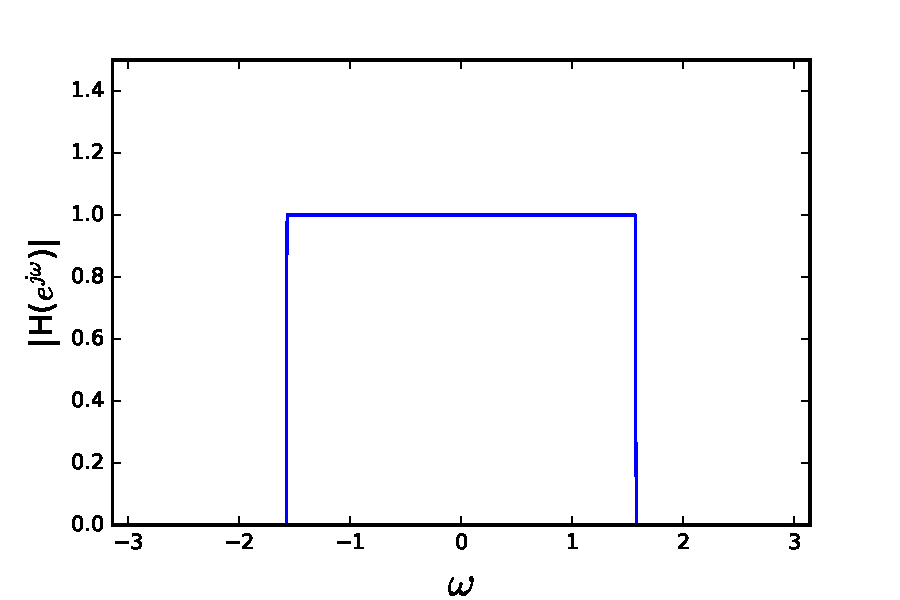
\includegraphics[scale=0.45]{figures/filter_teori/ideal_low2.pdf}
\caption{}
\end{subfigure}
\begin{subfigure}[b]{0.50\textwidth}
        \centering  
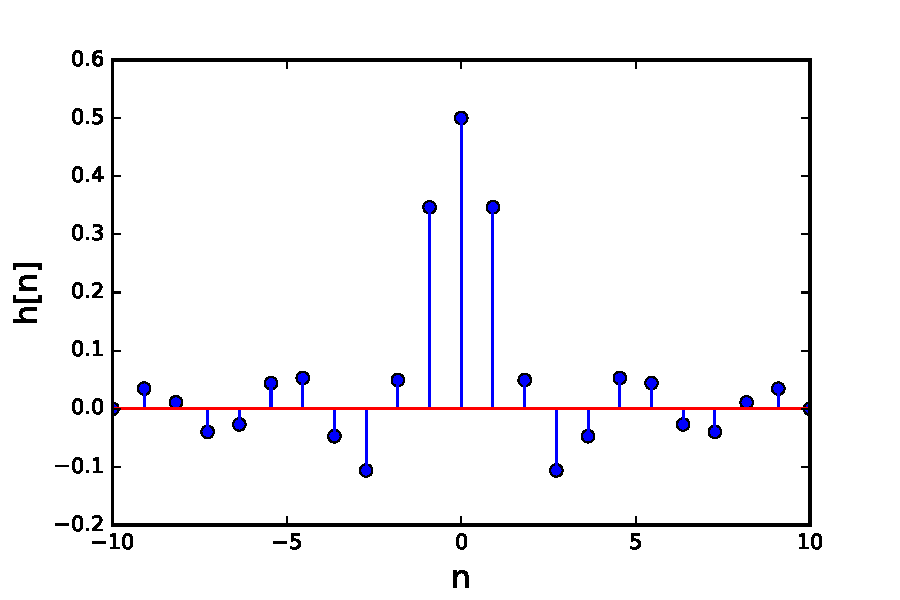
\includegraphics[scale=0.45]{figures/filter_teori/ideal_low1.pdf}
\caption{}
 \end{subfigure}
\caption{ (a) Amplitude response of ideal lowpass filter with $\omega_c = \frac{\pi}{2}$ (b) corresponding impulse response}
\label{fig:ideal_low}
\end{figure}


Analogues of ideal highpass or bandpass filter can be defined, as illustrated on figure \ref{fig:ideal}.\\ 

\begin{figure}[H]
\begin{subfigure}[b]{0.50\textwidth}
        \centering
\begin{tikzpicture}[scale=1]
\begin{axis}[
scale=0.5,
unit vector ratio*=1 1 1,
axis lines = middle,
xtick={1.5},
xticklabels={$\omega_c$},
ytick={1.5},
yticklabels={$1$},
xmin=0,
xmax=3,
ymin=0,
ymax=2.6]
\node at (axis cs:0.7,2.4) {$|H(\omega)|$};
\draw[line width=0.6mm](axis cs:0,0)--(axis cs:1.5,0);
\draw[line width=0.5mm](axis cs:1.5,1.5)--(axis cs:3,1.5);
\draw[line width=0.5mm](axis cs:1.5,1.5)--(axis cs:1.5,0);
\end{axis}
\end{tikzpicture}

\caption{}
    \end{subfigure}
 \begin{subfigure}[b]{0.50\textwidth}
        \centering  
\begin{tikzpicture}[scale=1]
\begin{axis}[
scale=0.5,
unit vector ratio*=1 1 1,
axis lines = middle,
xtick={1,2},
xticklabels={$\omega_a$,$\omega_b$},
ytick={1.5},
yticklabels={$1$},
xmin=0,
xmax=3,
ymin=0,
ymax=2.6]
\node at (axis cs:0.7,2.4) {$|H(\omega)|$};
\draw[line width=0.5mm](axis cs:1,1.5)--(axis cs:1,0);
\draw[line width=0.5mm](axis cs:1,1.5)--(axis cs:2,1.5);
\draw[line width=0.5mm](axis cs:2,1.5)--(axis cs:2,0);
\draw[line width=0.5mm](axis cs:1,0)--(axis cs:0,0);
\draw[line width=0.5mm](axis cs:2,0)--(axis cs:3,0);
\end{axis}
\end{tikzpicture}
\caption{}
    \end{subfigure}
\caption{Amplitude response of ideal (a) highpass filter (B) bandpass filter}
\label{fig:ideal}
\end{figure}
As stated in section \ref{sec:LTI} a non-causal LTI system is not realizable. Furthermore  zero phase is not possible for a causal system.
Thus an approximation of an ideal filter can be computed by a casual system with general linear phase.    

\section{FIR and IIR filter} 
Two classes of filter are essential to identify.
For all ideal filters discussed in the previous section the impulse response is defined for $-\infty < n < \infty$. Such a filter is specified as an \textit{infinite impulse response (IIR)} filter. In the case of the impulse response being zero outside a finite interval the filter is referred to as a \textit{finite impulse response (FIR)} filter. 
\subsection{Type 1 FIR filter}
As described causal systems with generalized linear phase is a possible approximation of the ideal filter. This is to be guaranteed by using specific types of FIR filters.\\
A causal system with generalized linear phase has to fulfil the following relation, cf. section \ref{sec:basic_filter}:
\begin{align}
\sum_{n=0}^{\infty}h[n]\sin\left(\omega \left(n-\alpha \right) + \beta \right) = 0
\end{align}
For a FIR filter to satisfy this relation the following set of conditions has to be fulfilled \cite{DTSP, p.342}:
\begin{align} \label{eq:FIR_con}
&\beta = \left\{ \begin{matrix} 
\pi  \\
0 
\end{matrix}\right. \nonumber  \\ 
&2\alpha = M = \text{an integer} \\ 
&h[n]=h[M-n] \ \text{or} \ h[n]=-h[M-n]. \nonumber  
\end{align} 
This implies that $h[n]$ is either symmetric or anti symmetric and that $\alpha = \frac{M}{2}$ becomes the symmetry point. \\
From these conditions four different types of FIR filter with generalized linear phase are defined \cite{DTSP, page 343}, only the \textit{type 1 FIR filter} will be elaborated here.
A type 1 FIR filter is characterised by having a symmetric impulse response and $M$ being an even integer. By applying the symmetry condition to the definition of the Fourier transform $H(\omega)$ is defined as \cite{page 343,DTSP}   
\begin{align}\label{eq:type1}
H(\omega)=\text{e}^{-j\omega \frac{M}{2}} \sum_{k=0}^{\frac{M}{2}} a[k]\cos \omega k,
\end{align}
where 
\begin{align}
a[k]= \left\{ \begin{matrix}
2h\left[ \frac{M}{2} - k \right], \ \ &\ k=1,2,... , \frac{M}{2}.   \\
h[\frac{M}{2}], \ \ &\ k = 0  
\end{matrix}\right.
\end{align}
By this \eqref{eq:type1} has the form of \eqref{eq:lin_pha} where $A(\omega)= \sum_{k=0}^{\frac{M}{2}} a[k]\cos \omega k$ is a real function of $\omega$ and $\beta$ equals either 0 or $\pi$. Hence a constant group delay is achieved.








   
 


 




\cleardoublepage
\chapter{System design and validation} \label{ch8}
With the concept and requirement for the system established in section \ref{sec:synth} and necessary theoretical knowledge obtained through chapter \ref{ch4} to \ref{ch7} system design are to be set up in this chapter. Test for validation of each unit will be carried out and documented along with the design process according to the test specifications in section \ref{sec:testspec}. One section is allocated to each software unit in the application cp. section \ref{sec:testspec}. The chapter concludes with a test of the final system followed by an evaluation.  \\

\section{Fourier transformation - FFT}

\section{Filter}
The filter design process is documented in this section, which includes determination of filter specifications, implementation and test. As stated in section \ref{sec:filtervalg} a bandpass FIR filter of type I designed with use of a Kaiser window is wanted.

\subsection{Specifications of filter} \label{sec:FIRspec} 
The purpose of this filter is to remove all frequencies outside the passband of the filter.  \\
Due to the frequency analysis in section ~\ref{sec:single} the main energy in the analysed signals is located within a frequencyband from 75 Hz to 1000 Hz.  
By letting the cut-off frequencies $f_c$ of the filter be respectively 75 Hz and 1000 Hz, this makes the passband of the filter. \\ 
According to section \ref{subsec:FIR} the Kaiser window can be determined from specifications of the allowed transition width $tw$ and peak approximation error $\delta$ of the amplitude in the pass- and stopbands. \\ 
By the frequency analysis of different types of noise it is found that the frequency spectrum of the music signal leis within the frequency spectrum of the noise which verifies the need of a narrow transitionband. However, the narrower transitionband means the higher order of filter is needed, which gives more computations, and hence it is not realistic to let the width of the transitionband go toward zero.  \\
The maximum allowed width of the transitionband $tw$ and peak approximation error in amplitude $\delta$ is determined as
\begin{align}
tw = 20 \ Hz, \ \ \ \ \  \delta = 0.05. 
\end{align}
The amplitude response of the ideal filter is sketched in figure \ref{fig:spec_Hd} along with the boundaries for the real filter as provided by the defined specifications.      

\begin{figure}[H]
\centering
\begin{tikzpicture}[scale=1]
\begin{axis}[every tick/.style={blue, ultra thick}, 
scale=1.1,
unit vector ratio*=1 1 1,
axis lines = middle,
x label style={at={(current axis.right of origin)},anchor=north},
xlabel={$[Hz]$},
xtick={2,5,10,13},
xticklabels={$f_{c1}-\frac{tw}{2}$,$f_{c1}+\frac{tw}{2}$,$f_{c2}-\frac{tw}{2}$,$f_{c2}+\frac{tw}{2}$},
ytick={0.5,3,4},
yticklabels={$\delta_1$,$1-\delta_1$,$1+\delta_1$},
xmin=0,
xmax=16,
ymin=-1,
ymax=5.5]
\node at (axis cs:1.9,4.9) {$|H_d(2\pi f)|$};
\draw[line width=0.5mm](axis cs:0,0)--(axis cs:3.5,0);
\draw[line width=0.5mm](axis cs:3.5,0)--(axis cs:3.5,3.5);
\draw[line width=0.5mm](axis cs:3.5,3.5)--(axis cs:11.5,3.5);
\draw[line width=0.5mm](axis cs:11.5,3.5)--(axis cs:11.5,0);
\draw[line width=0.5mm](axis cs:11.5,0)--(axis cs:16,0);
\draw[line width=0.25mm, dashed](axis cs:0,0.5)--(axis cs:2,0.5);
\draw[line width=0.25mm, dashed](axis cs:13,0.5)--(axis cs:16,0.5);
\draw[line width=0.25mm, dashed](axis cs:5,3)--(axis cs:10,3);
\draw[line width=0.25mm, dashed](axis cs:2,4)--(axis cs:13,4);
\draw[line width=0.25mm](axis cs:2,0.5)--(axis cs:2,4);
\draw[line width=0.25mm](axis cs:5,0)--(axis cs:5,3);
\draw[line width=0.25mm](axis cs:10,0)--(axis cs:10,3);
\draw[line width=0.25mm](axis cs:13,4)--(axis cs:13,0.5);
%\draw[line width=0.5mm](axis cs:4,0.5)--(axis cs:7,0.5);
%\node at (axis cs:1,1.5) {Passband};
%\node at (axis cs:3,1.5) {Transition};
%\node at (axis cs:5.0,1.5) {Stopband};
\end{axis}
\end{tikzpicture}
\caption{Amplitude response of ideal filter within the boundaries for the amplitude response of the realizable filter as given by the defined specifications.}
\label{fig:spec_Hd}
\end{figure}

\subsection{Implementation of filter}
The implementation of the filter basically follows algorithm \ref{alg:FIR}. The ideal impulse response is defined as the inverse Fourier transformation of the ideal filter specified in figure \ref{fig:spec_Hd}. The derivation of the ideal impulse response of a bandpass filter is shown in appendix \ref{appC}. From the given specifications the shape parametere of the kaiser window becomes $\beta \approx 1.5$ which gives a filter order of 2766. Figure \ref{fig:FIRimpulse} show the impulse response of the filter. Figure \ref{fig:freq_filt1} illustrates a plot of the amplitude response corresponding to the filter in the frequency domain. Figure \ref{fig:freq_filt2} illustrates a close-up view of the left transitionband, showing the ripples in the stop- and passband. The boundaries from the specifications are marked by the green lines. It is seen that the specifications are fulfilled. 
\begin{figure}[h]
\centering 
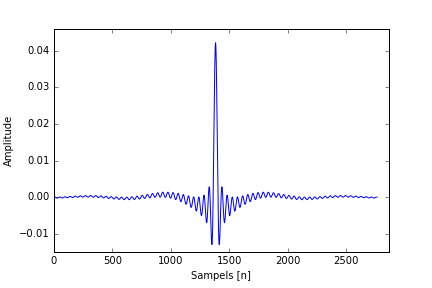
\includegraphics[scale=0.4]{figures/filtertest/impulse.png}
\caption{Impulse response of filter with order $M=2766$}
\label{fig:FIRimpulse}
\end{figure}
       
\begin{figure}[h]
\centering
\begin{subfigure}{0.49\textwidth}
\centering
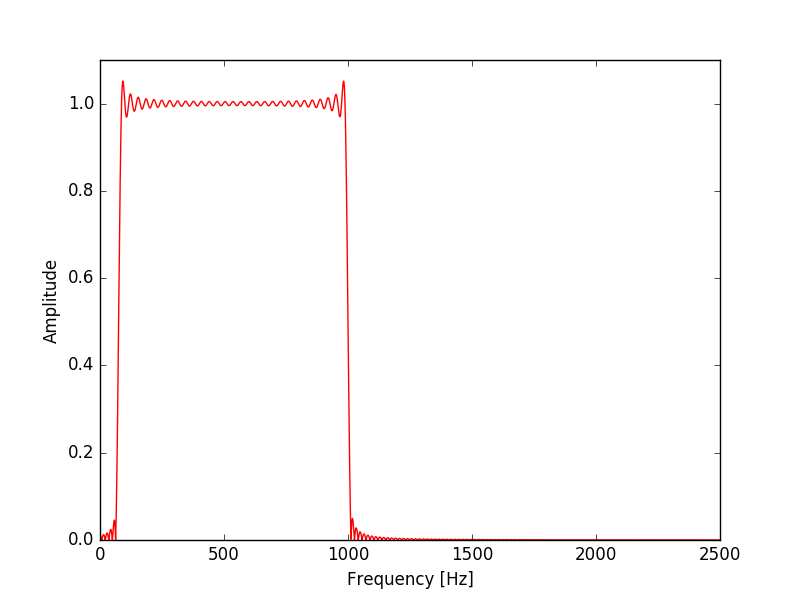
\includegraphics[width=\textwidth]{figures/filtertest/freq_response1.png}
\caption{}
\label{fig:freq_filt1}
\end{subfigure}
\begin{subfigure}{0.49\textwidth}
\centering
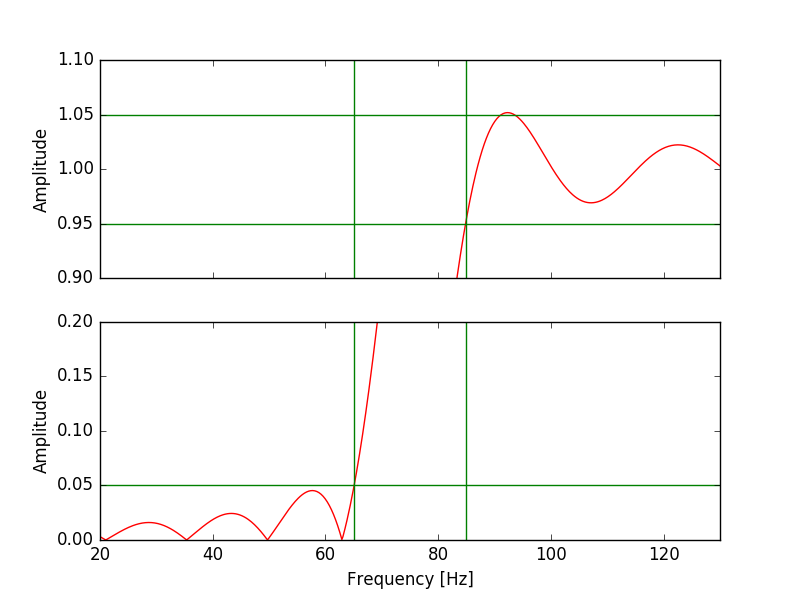
\includegraphics[width=\textwidth]{figures/filtertest/freq_response2.png}
\caption{}
\label{fig:freq_filt2}
\end{subfigure}
\caption{(a) Amplitude response of filter. (b) Close-up view of amplitude response of filter, showing top and bottom of one transitionband.}
\label{fig:freq_filt}
\end{figure}

\begin{algorithm}[H]
\caption{Compute type I FIR filter}
\label{alg:FIR}
\begin{algorithmic}[1] 
\Procedure{Compute kaiser window $w$}{}
\State $A=-20\log_{10}(\delta)$ \Comment{$21 \leq A \leq 50$}
\State $\beta = 0.5824(A-21)^{0.4} + 0.07886(A-21)$ \Comment {Shape parameter}
\State $M = (A-8)/(2.285 \cdot \frac{tw}{f_s} 2\pi)$ \Comment {Filter order, round to upper even int.}
\State $N = M+1$ \Comment {Length of filter}
	\For {each $i$ in length of $N$}
		\For {each $j$ in length of $M$}
			\State $ sum_n + = \ (\frac{1}{j!})^2 \left( \left( \frac{\beta}{2} \sqrt{\left(1 - \left( \frac{2 \cdot i}{N-1}\right) - 1\right)^2}\right)^{2j}\right)$
			\State $ sum_d + = \ (\frac{1}{j!})^2 \left( \frac{\beta}{2}\right)^{2j}$
		\EndFor
		\State $w[i]=\frac{sum_n}{sum_d}$
	\EndFor
	\State Return $w$, $M$
\EndProcedure
\\
\Procedure{Compute ideal impulse response $h_d$}{}
   \For {each $i$ in length of $N$}
        \If {$i == \frac{M}{2}$}
        		\State $h_d[i] = 2( \frac{f_{c2}}{f_s} - \frac{f_{c2}}{f_s})$
        	\Else 
        		\State  $h_d[i] = \frac{1}{ (\pi (i - \frac{M}{2}))}(\sin(\frac{f_{c2}}{f_s} 2 \pi (i - \frac{M}{2})) - (\sin(\frac{f_{c1}}{f_s} 2 \pi (i - \frac{M}{2}))))$ 
          	\EndIf 
  	\EndFor
  	\State Return $h_d$
\EndProcedure
\\
\Procedure{Compute impulse response $h$}{}
	\State Return $h = h_d \cdot w$ \Comment{Windowed impulse response}
\EndProcedure


\end{algorithmic}
\end{algorithm}

\subsection{Test of the filter}
The implemented filter is tested according to the test specifications described in section \ref{sec:testspec}. Figure \ref{fig:SIGNAL} shows the frequency spectrum of the single low E tone with additive noise in form of a beat of hands clapping. Figure \ref{fig:filt_SIGNAL} shows the filtered signal. Note that the frequency spectrum are only showed from 0 to approximately 2200 Hz.  

\begin{figure}[H]
\centering
\begin{subfigure}{0.49\textwidth}
\centering
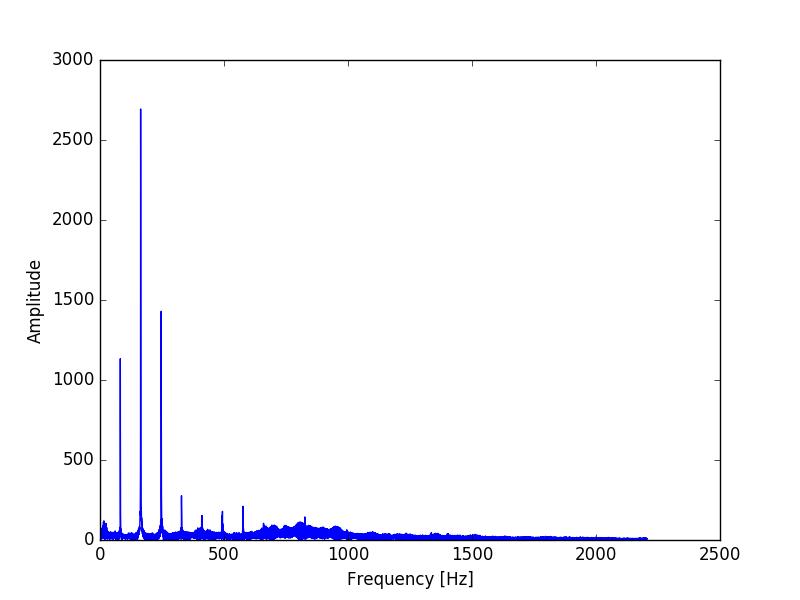
\includegraphics[width=\textwidth]{figures/filtertest/SIGNAL.png}
\caption{}
\label{fig:SIGNAL}
\end{subfigure}
\begin{subfigure}{0.49\textwidth}
\centering
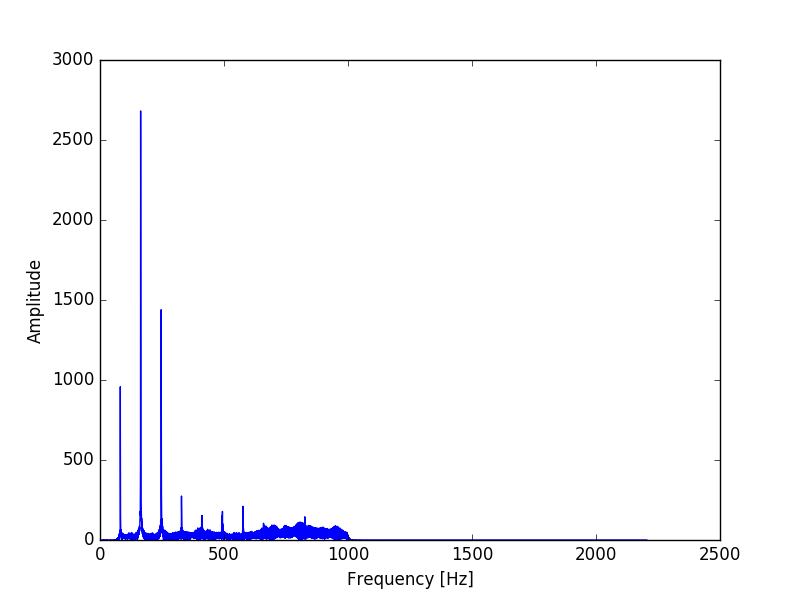
\includegraphics[width=\textwidth]{figures/filtertest/filt_SIGNAL.png}
\caption{}
\label{fig:filt_SIGNAL}
\end{subfigure}
\caption{(a) Frequency spectrum of signal with noise. (b) Frequency spectrum of filtered signal.}
\label{fig:test_res}
\end{figure}
As described in the specifications the filter is designed to remove all frequencies outside the frequencyband from 75 Hz to 1000 Hz. It is seen by comparing figure \ref{fig:SIGNAL} and figure \ref{fig:filt_SIGNAL} that the frequencies outside the passband appears to be zero and that the amplitudes of the remaining frequencies are appropriately the same. \\
By this the designed filter of order 2766 fulfil the specifications and the implementation of the filter works as intended. \\

\section{STFT}

\section{Spectrogram}

\section{Integration validation}

\section{Final system test}


\cleardoublepage
\chapter{Frequency analysis} \label{ch9}
In this chapter the results from the recordings described in appendix \ref{recordings} will undergo frequency analyses. This will detect the frequency compositions of the music and noise signals, which will aid the design of a filter designated to filter out noise. The frequency analyses is furthermore necessary for the creation of spectrograms illustrating the frequency compositions of the signals in time. \\ \\
This project includes an implementation of the Cooley-Tukey FFT algorithm in Python but the results of this algorithm are identical to the FFT included in the Numpy-package in Python, which is much faster than the implementation described in algorithm \ref{FFTalg}. The FFT from Numpy will therefore be used for the frequency analyses in this chapter.

\section{Frequency analysis of music}
In this section the recordings of music will undergo frequency analysis, and the goal is to be able to express which frequencies the tones played in the recordings are generally found at. It is expected that both the significant tone and its corresponding harmonics will appear in the frequency spectrum.
   
\subsection{Single tone} \label{sec:single}
Firstly, the tuning of guitar is checked for consistency. The low and high E strings on the guitar should vibrate and emit sounds frequencies of 82.41 Hz and 329.63 Hz, respectively, as seen in table \ref{fig:guitar_frequencies}. Figures \ref{fig:single_low} and \ref{fig:single_high} show the frequency spectra for the recordings of the two tones.
\begin{figure}[H]
\centering
\begin{subfigure}{0.49\textwidth}
\centering
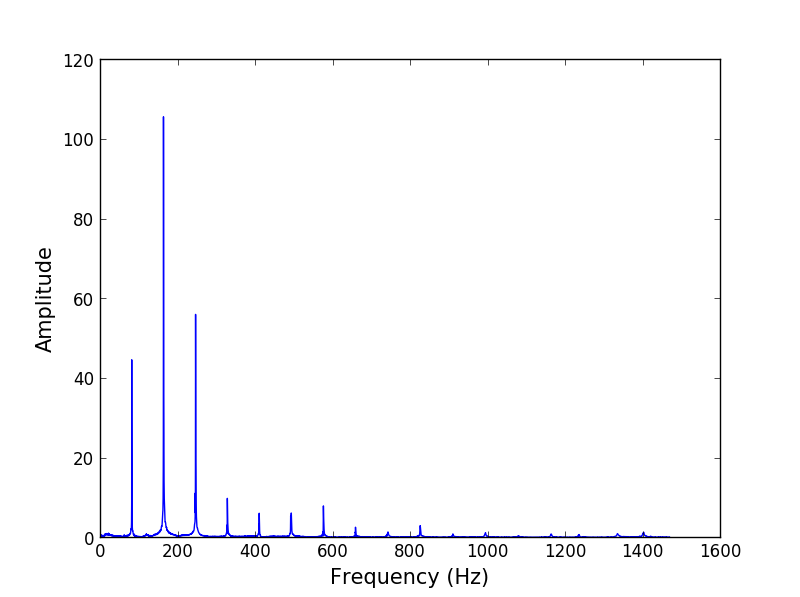
\includegraphics[width=\textwidth]{figures/freqanal/single_low.png}
\caption{Low E string}
\label{fig:single_low}
\end{subfigure}
\begin{subfigure}{0.49\textwidth}
\centering
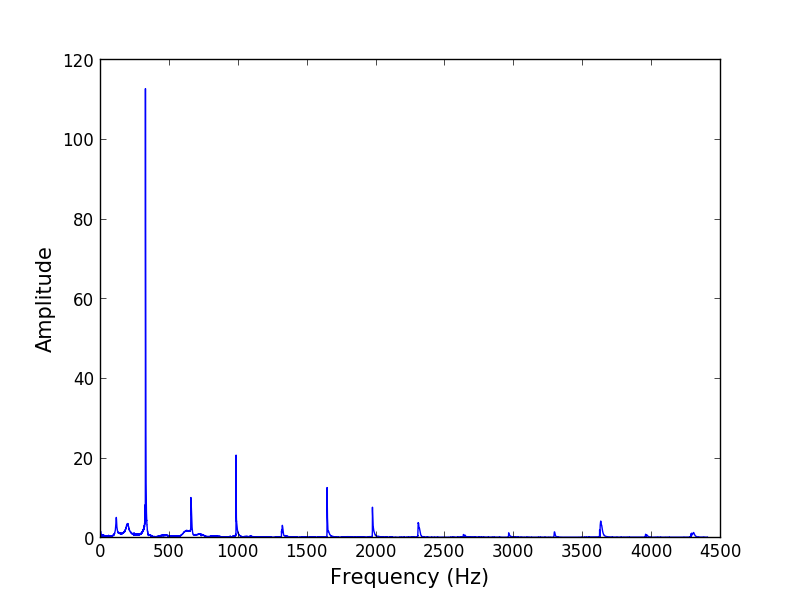
\includegraphics[width=\textwidth]{figures/freqanal/single_high.png}
\caption{High E string}
\label{fig:single_high}
\end{subfigure}
\caption{Frequency spectra of low and high E strings on a guitar. The harmonics are clearly visible.}
\label{fig:single}
\end{figure}
\martin{Frederik retter de her grumme figurer.}

With a peak detection algorithm implemented in Python the most significant frequencies in the two recordings are registered to be 163.82 Hz and 329.83 Hz for the low and high E's, respectively. As $163.82$ Hz $\approx 2\cdot82.41$ Hz this is regarded as a harmonic of the low E. The harmonics are moreover observable in the figures as reduced peaks at integer multiples of the fundamental frequencies of the tones. It is furthermore seen from the figures, that the energy in the signals is mainly located at frequencies above 75 Hz and below 1000 Hz for the low E and above 100 Hz and below 2000 Hz for the high E.\\ 

\subsection{Chord}
Figures \ref{fig:chord_low} and \ref{fig:chord_high} show the frequency spectra of the recordings of low and high E chords, respectively.
\begin{figure}[H]
\centering
\begin{subfigure}{0.49\textwidth}
\centering
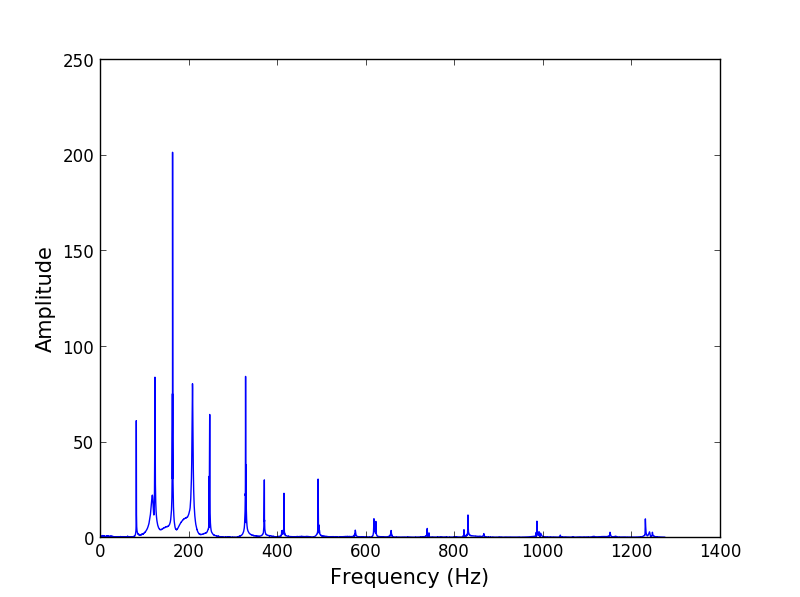
\includegraphics[width=0.9\textwidth]{figures/freqanal/chord_low.png}
\caption{Low E chord.}
\label{fig:chord_low}
\end{subfigure}
\begin{subfigure}{0.49\textwidth}
\centering
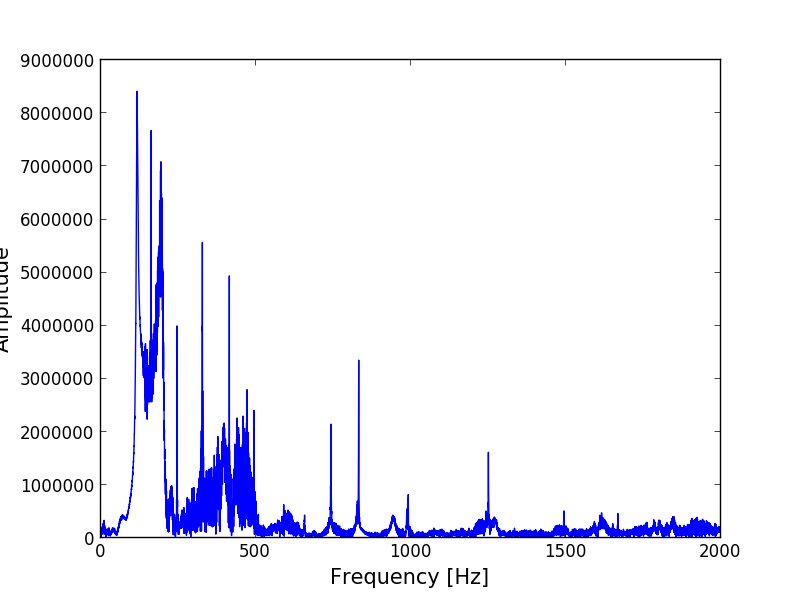
\includegraphics[width = \textwidth]{figures/freqanal/chord_high.png}
\caption{High E chord.}
\label{fig:chord_high}
\end{subfigure}
\caption{Frequency spectra of low and high E chords played on a guitar.}
\label{fig:chord}
\end{figure}

The most significant frequencies in figure \ref{fig:chord_low} is 163.86 Hz and 119.27 Hz in figure \ref{fig:chord_high}. Once again it is assumed that the higher frequency of the low pitch E is due to harmonics. The second frequency does furthermore not correspond to a specific note - this is assumed to be because of the composition of chords being of multiple tones. The majority of the energy in the signals is located above 80 Hz and below 1000 Hz.
\subsection{Scale}
Figure \ref{fig:scale_fast} shows the frequency spectrum of playing a octatonic scale.
\begin{figure}[H]
\centering
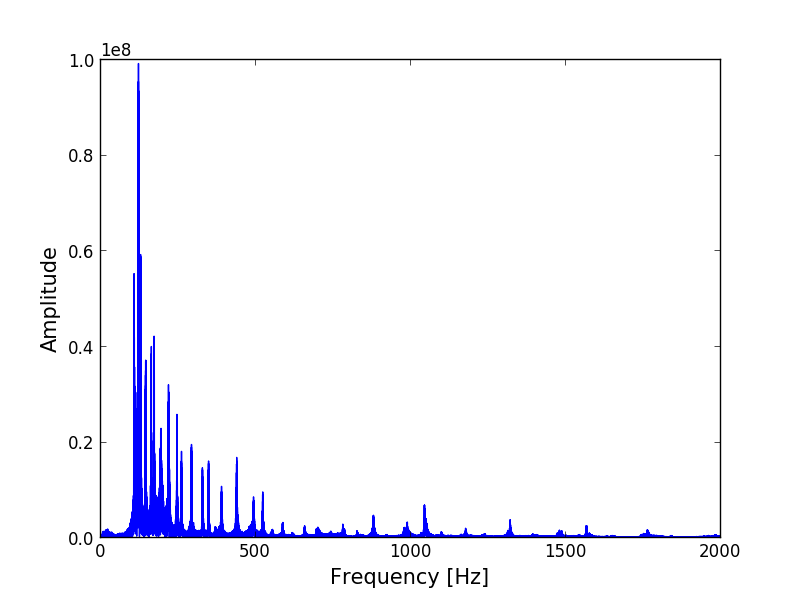
\includegraphics[width=0.7\textwidth]{figures/freqanal/scale_fast.png}
\caption{Frequency spectrum of an octatonic scale played quickly.}
\label{fig:scale_fast}
\end{figure}
The majority of the energy in the signal is as seen located above 100 Hz and below 600 Hz.

\subsection{Melody with single notes}
Figures \ref{fig:melody_single} show the frequency spectrum for a melody consisting only of single tones played slowly.
\begin{figure}[H]
\centering
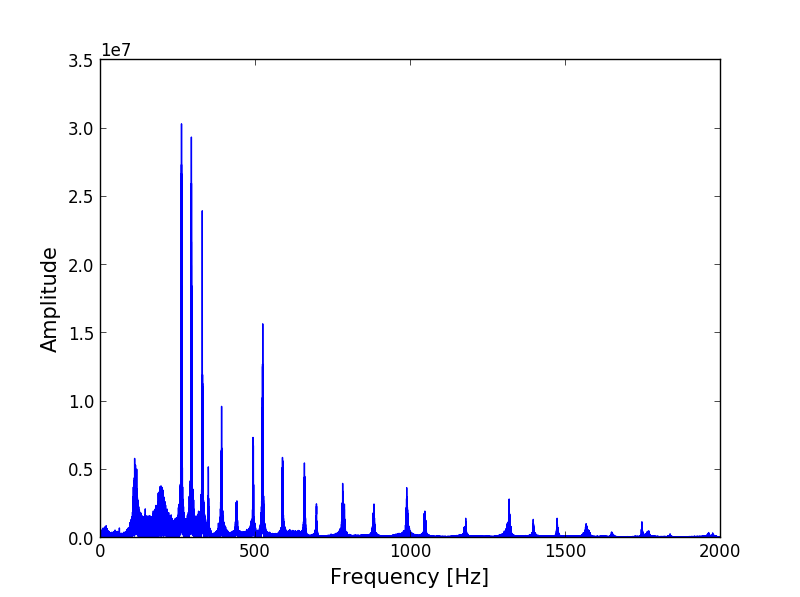
\includegraphics[width=0.7\textwidth]{figures/freqanal/melody_single.png}
\caption{Frequency spectrum of Itsy Bitsy Spider played on a guitar with only single strings plucked.}
\label{fig:melody_single}
\end{figure}
The majority of energy in the signal is located above 100 Hz and below 2000 Hz.

\section{Frequency analysis of noise}
In this section the recordings of noise will undergo frequency analysis, and the goal is to be able to express which frequencies the recorded noise is generally found at.
\subsection{Folding paper and clapping}
Figure \ref{fig:clapping} and \ref{fig:folding} show the frequency spectrum of clapping at equidistant intervals in time and folding a piece of paper, respectively.
\begin{figure}[H]
\centering
\begin{subfigure}{0.49\textwidth}
\centering
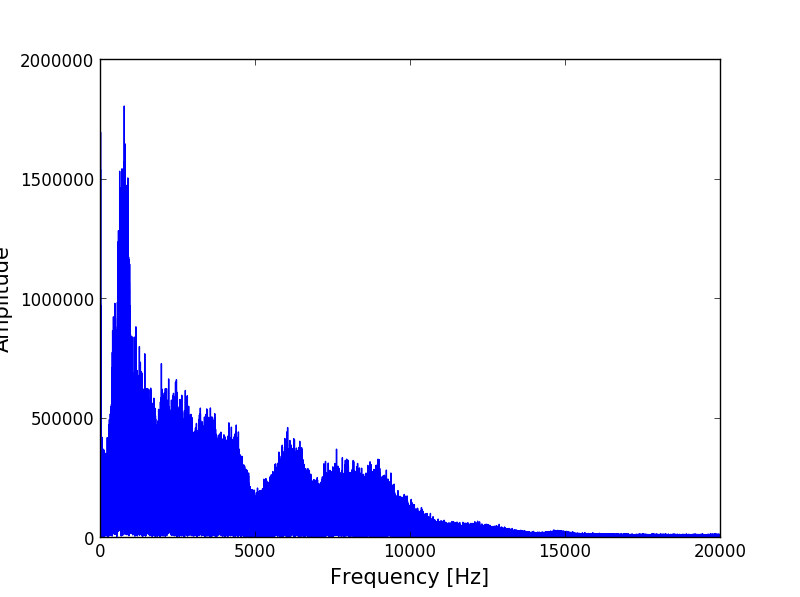
\includegraphics[width=\textwidth]{figures/freqanal/clapping.png}
\caption{Clapping}
\label{fig:clapping}
\end{subfigure}
\begin{subfigure}{0.49\textwidth}
\centering
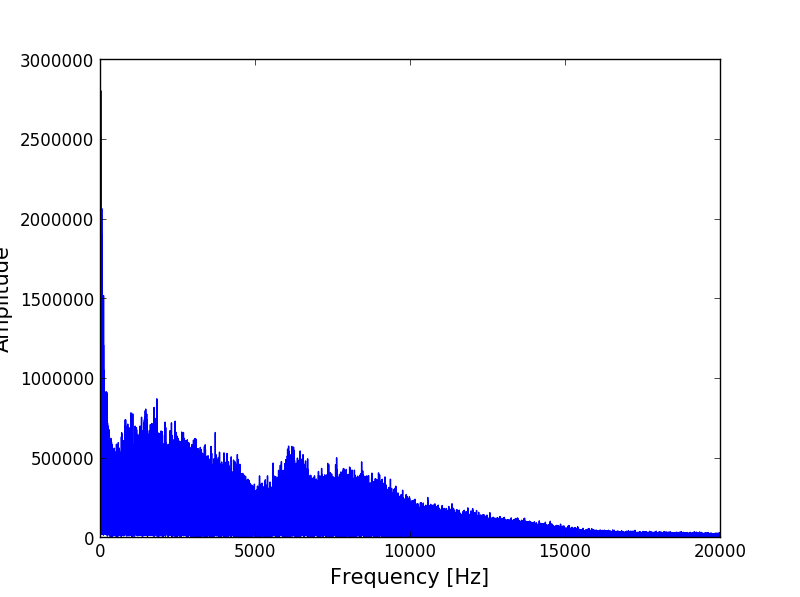
\includegraphics[width=\textwidth]{figures/freqanal/folding.png}
\caption{Folding a piece of paper}
\label{fig:folding}
\end{subfigure}
\caption{Frequency spectra of different noises.}
\end{figure}
The majority of the energy in both noises is located between 0 and 15000 Hz.
%\subsection{Singing and talking}
%Figures \ref{fig:talk} and \ref{fig:song} show the frequency spectrum of recorded talking and singing respectively.
%\begin{figure}[H]
%\centering
%\begin{subfigure}{0.49\textwidth}
%\centering
%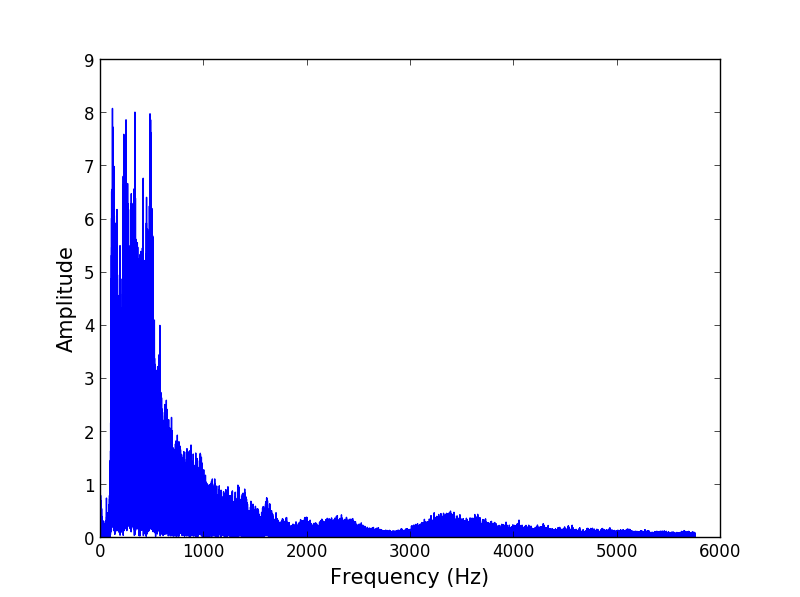
\includegraphics[width=\textwidth]{figures/freqanal/talk.png}
%\caption{Person talking}
%\label{fig:talk}
%\end{subfigure}
%\begin{subfigure}{0.49\textwidth}
%\centering
%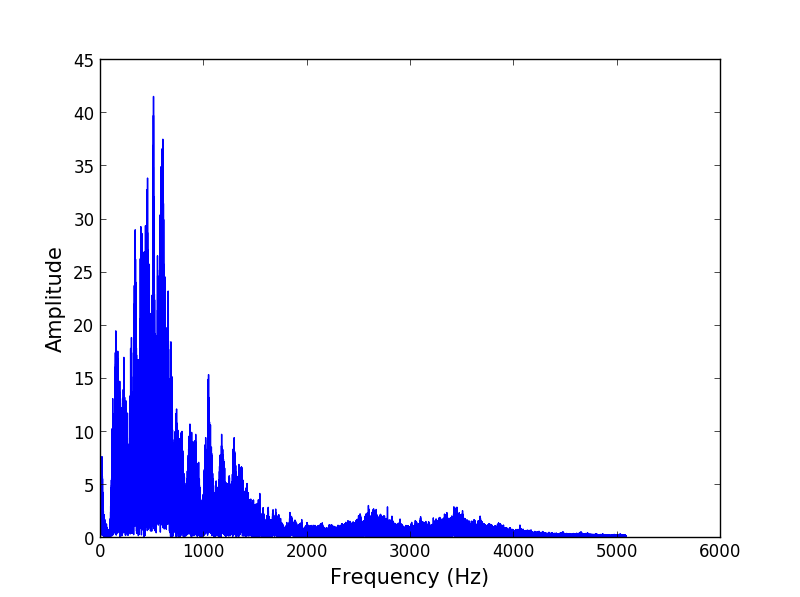
\includegraphics[width=\textwidth]{figures/freqanal/song.png}
%\caption{Person singing}
%\label{fig:song}
%\end{subfigure}
%\caption{Frequency spectra of a person talking and signing.}
%\end{figure}
%The majority of the energy is located between 100 and 5000 Hz for talking and 0 and 5000 Hz for singing.
\subsection{Ambient noise}
Figure \ref{fig:ambient} shows the frequency spectrum of the ambient noise recorded in a parking lot at the campus of AAU.
\begin{figure}[H]
\centering
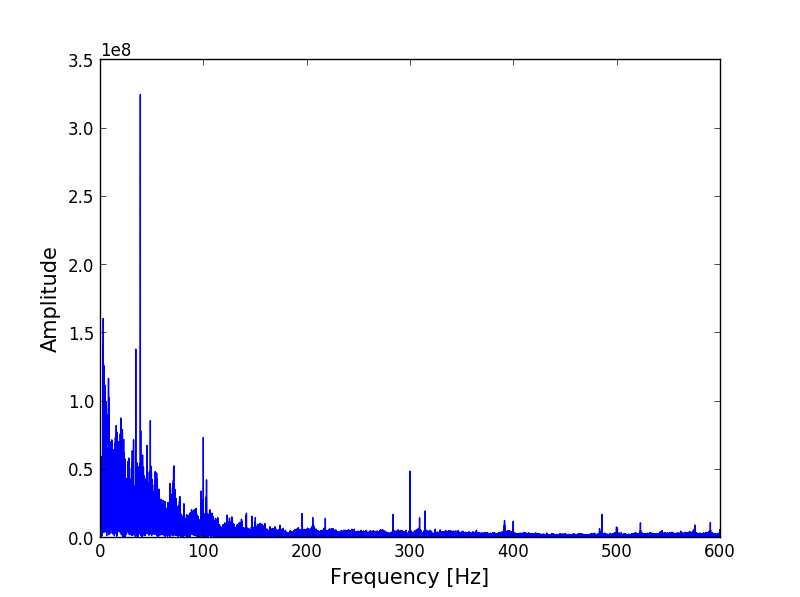
\includegraphics[width=0.7\textwidth]{figures/freqanal/ambient.png}
\caption{Frequency spectrum for ambient sound.}
\label{fig:ambient}
\end{figure}
The majority of the energy in the signal is located between 0 and 600 Hz.













\section{Filter design}
In this section, the frequency analysis of the music and noise in the former sections form the basis for the design of the filter, whose aim is to filter out the noise. The noise is both low- and high-frequency, whereas the frequency of the music lies in the middle, which means that the filter should be a bandpass filter. From the discussion of different filters and designs of these in chapter \ref{ch8} the implemented filter is furthermore chosen to be a FIR filter since this type of filter is guaranteed to have linear phase, which preserves the wave form of the original signal, which of course is important in this project. Furthermore, FIR filters are rather easy to design. On the downside, a FIR filter uses many computations, which is problematic if the filter is supposed to run in real time - that is, while the music is being played. However, in this project the music is first recorded and then analysed, which means that the computations are not a big factor. For an actual system working in real time the amount of computations plays a bigger factor, and such a system could be considered to use an IIR filter but the linear phase from the FIR filter is weighted as more important in this particular project.
\cleardoublepage
\chapter{System design and validation} \label{ch10}
With the concept and requirement for the system established in section \ref{sec:synth} and necessary theoretical knowledge obtained through chapter \ref{ch4} to \ref{ch7} system design are to be set up in this chapter. Test for validation of each unit will be carried out and documented along with the design process according to the test specifications in section \ref{sec:testspec}. One section is allocated to each software unit in the application cp. section \ref{sec:testspec}.The chapter concludes with a test of the final system followed by an evaluation.  \\


\section{Fourier transformation - FFT}
\section{FFT}
This section describes the implementation of the FFT discussed in section \ref{sec:FFT}, which uses an implementation of the DFT discussed in section \ref{sec:DFT}. The implementation of the FFT is assessed by comparing both the computational efforts and the results of the implementations of the DFT and FFT compared to Numpy's FFT. The results are expected to be similar since the FFT is a fast way of calculating the DFT.

\subsection{Implementation of the FFT}
Firstly, the implementation of the DFT is described in the following algorithm.
\begin{algorithm}
\caption{DFT algorithm}
\label{DFTalg}
\begin{algorithmic}[1]
\State $N =$length of $x$ \Comment{Number of samples to be computed}
\Procedure{Compute DFT}{x,N}
	\State{$X = $np.zeros$(N,$dtype=complex$)$}
	\For{k between 0 and length of signal}
		\State{$a = 0 + 0\cdot j$} \Comment{$a$ is zero but of type complex}
		\For{n between 0 and N}
			\State{$a += x[n]\cdot \exp(-2\cdot \pi\cdot j 					\cdot k \cdot n/$float$(c))$}
			\State{$X[k] = a$}
		\EndFor
	\EndFor
	\State {Return $X$}
\EndProcedure
\end{algorithmic}
\end{algorithm}

The implementation of the FFT shown in the following algorithm uses a function to make sure that the number of samples to be computed is a power of 2 (as described in section \ref{sec:FFT}). This function asks if $N$ is positive and a power of 2. If not, the function returns a False-statement, which raises a \textit{Valueerror} in the FFT algorithm. However, the FFT function from the Numpy-package uses zeropadding to modify a signal of arbitrary length into a signal with a length that is a power of 2. That has not been implemented in the FFT shown below. In the FFT algorithm shown below, the signal is divided into even and odd samples if the signal is more than 2 samples long, which are computed separately by using the FFT itself; if the number of even (and odd) samples are still more than 2 the samples are divided even further until the number of even (and odd) samples are 2. These samples are then computed by the DFT described in algorithm \ref{DFTalg}. After dividing the samples into even and odd samples the twiddle factor is multiplied appropiately (as described in section \ref{sec:FFT}), and eventually the Numpy-function \textit{concatenate} is used to join the arrays back together.\martin{Hvad betyder \& i algoritmen?}
\begin{algorithm}
\caption{FFT algorithm}
\label{FFTalg}
\begin{algorithmic}[1]

\Procedure{Power of 2}{N}
	\State{Return $N$!=$0$ and $(N \& (N - 1)) == 0$}
\EndProcedure

\Procedure{Compute FFT}{x}
	\State $N$ = length of $x$ 
	\If{Power of 2($N$) == False }
		\State{Raise Valueerror(``N should be a power of 2.'')}
	\ElsIf{$N$ == 2}
		\State{Return DFT($x$,$N$)} \Comment{$x$ is the signal}
	\Else
		\State{$X_{e} = FFT(x[::2])$} \Comment{The even 				samples}
		\State{$X_{o} = FFT(x[1::2])$} \Comment{The odd 				samples}
		\State{$factor = \exp(-2j\cdot \pi \cdot 						$np.arange$(N) / N)$} \Comment{The twiddle 			factor}
		\State{Return np.concatenate$([X_{e} + factor[: 	N/ 2] \cdot X_{o}, X_{e} +  factor[N / 2:] \cdot X_{o}])$}
	\EndIf
\EndProcedure
\end{algorithmic}
\end{algorithm}

\subsection{Test of the FFT}
The FFT algorithm above is compared to both the DFT algorithm and the FFT function from the Numpy-package by measuring how long it takes for the functions to compute different amounts of random numbers. This is shown in table \ref{tab:FTcompare}. Furthermore, the algorithms are compared by their outputs.

\begin{table}[H]
\centering
\begin{tabular}{|l|l|l|l|}
\hline
Type / $N$ & DFT	   & FFT 	 & Numpy's FFT \\ \hline
$2^9$  	   & $1.03$    & $0.01$  & $\sim 0.00$ \\ \hline
$2^{10}$   & $4.43$    & $0.02$  & $\sim 0.00$ \\ \hline
$2^{11}$   & $17.36$   & $0.03$  & $\sim 0.00$ \\ \hline
$2^{12}$   & $69.42$   & $0.07$  & $\sim 0.00$ \\ \hline
$2^{13}$   & $290.89$  & $0.18$  & $\sim 0.00$ \\ \hline
$2^{14}$   & $1206.85$ & $0.27$  & $\sim 0.00$ \\ \hline
\end{tabular}
\caption{Times in seconds it take for the implementations of the DFT, the FFT and Numpy's FFT to compute $N$ random numbers. Processor used: Intel Core I5 generation 5 with CPU of 2.20 GHz.}
\label{tab:FTcompare}
\end{table}

Table \ref{tab:FTcompare} shows that the time the DFT takes to compute the $N$ numbers grows rapidly, whereas either of the FFTs take less than a second. The values for Numpy's FFT are rounded off to zero, and this function's ability to rapidly perform the computations is due to the fact that Numpy actually performs the computations in C, where the code is already compiled and runs directly on the CPU. On the other hand, Python is an interpreted language, which means that each line of the code has to be translated before it can be run. However, that obviously does not mean that the implementation of the FFT shown above is slow, and it is certainly much faster than the implementation of the DFT. \\
It is furthermore interesting to examine whether this result corresponds to the theoretical relation of the computational complexities. From section \ref{sec:FFT} the theoretical numbers of arithmetic operations required to compute the DFT and FFT are $N^2$ and $N\log_2(N)$, respectively. The relation $\frac{N^2}{N \cdot \log_2(N)}$ of these computational complexities equals $\frac{N}{\nu}$ for $N = 2^\nu, \nu \in \mathbb{N}$, which is a 


  
For $N=2^9$ this gives an approximate relation of the FFT being $57$ times faster than the DFT but the actual relation is $103/1$ from table \ref{tab:FTcompare}. From this the computation of the implemented FFT is approximately twice as fast as found theoretically compared to the implemented DFT, which is due to the number of computations and the computer's processing time cannot be directly compared \martin{Martin udvider sammenligningen af tallene}. \\
\\
The implementation of the FFT and Numpy's FFT should also be compared for larger number of samples $N$ since e.g. $N = 2^{19}$ is 11.89 seconds with a sampling frequency of 44100 Hz, which is a reasonable length of an audio file from the recordings described in appendix \ref{recordings}. The DFT will obviously take too long and is therefore not included in the comparison in table \ref{tab:FT2compare}.

\begin{table}[H]
\centering
\begin{tabular}{|l|l|l|l|}
\hline
Type / $N$ & FFT	   & Numpy's FFT \\ \hline
$2^{18}$   & $5.15$    & $0.03$ \\ \hline
$2^{19}$   & $9.79$    & $0.04$ \\ \hline
$2^{20}$   & $19.74$   & $0.14$ \\ \hline
$2^{21}$   & $40.31$   & $0.26$ \\ \hline
$2^{22}$   & $79.59$   & $0.56$ \\ \hline
$2^{23}$   & $159.39$  & $1.08$ \\ \hline
\end{tabular}
\caption{Times in seconds it take for the implementation of the FFT and Numpy's FFT to compute $N$ random numbers. Processor used: Intel Core I5 generation 5 with CPU of 2.20 GHz.}
\label{tab:FT2compare}
\end{table}

Obviously, the implementation of the FFT takes rather long for large numbers of samples, whereas Numpy's FFT only takes a little more than a second. It should be noted that the results above cannot be reproduced exactly since the numbers are random and the same amount of different numbers results in slightly different times of computations. Also, one might check the validity of the DFT and FFT algorithms by comparing the result of the algorithms and Numpy's FFT by using the Numpy function \textit{np.allclose}. An example is \textit{np.allclose(FFT(x),np.fft.fft(x))}, which returns a True-statement if the results of $FFT(x)$ described in algorithm \ref{FFTalg} and Numpy's FFT are similar to a certain degree$^[$\footnote{See also the documentation for the \textit{allclose}-function on \href{https://docs.scipy.org/doc/numpy/reference/generated/numpy.allclose.html}{https://docs.scipy.org}.}$^]$. This was always the case in the comparison of the implementations of the DFT, the FFT and Numpy's FFT described above.
\\ \\
Therefore, the implementation of the DFT and FFT described in algorithm \ref{DFTalg} and \ref{FFTalg}, respectively, returns the exact same values as Numpy's FFT. The DFT is obviously extremely slow for even rather small numbers of samples, and the FFT is also rather slow compared to Numpy's FFT for large numbers of samples.
\\ \\
Because Numpy's FFT is so much faster than the implemented FFT and because Numpy's FFT is capable of zeropadding and thus computing a signal of any length, it is decided to use Numpy's FFT in the future processings of the signals in this report \martin{Nyt. \textregistered}.

\section{Filter}
The filter design process is documented in this section, which includes determination of filter specifications, implementation and test. As stated in section \ref{sec:filtervalg} a bandpass FIR filter of type I designed with use of a Kaiser window is wanted.

\subsection{Specifications of filter} \label{sec:FIRspec} 
The purpose of this filter is to remove all frequencies outside the passband of the filter.  \\
Due to the frequency analysis in section ~\ref{sec:single} the main energy in the analysed signals is located within a frequencyband from 75 Hz to 1000 Hz.  
By letting the cut-off frequencies $f_c$ of the filter be respectively 75 Hz and 1000 Hz, this makes the passband of the filter. \\ 
According to section \ref{subsec:FIR} the Kaiser window can be determined from specifications of the allowed transition width $tw$ and peak approximation error $\delta$ of the amplitude in the pass- and stopbands. \\ 
By the frequency analysis of different types of noise it is found that the frequency spectrum of the music signal leis within the frequency spectrum of the noise which verifies the need of a narrow transitionband. However, the narrower transitionband means the higher order of filter is needed, which gives more computations, and hence it is not realistic to let the width of the transitionband go toward zero.  \\
The maximum allowed width of the transitionband $tw$ and peak approximation error in amplitude $\delta$ is determined as
\begin{align}
tw = 20 \ Hz, \ \ \ \ \  \delta = 0.05. 
\end{align}
The amplitude response of the ideal filter is sketched in figure \ref{fig:spec_Hd} along with the boundaries for the real filter as provided by the defined specifications.      

\begin{figure}[H]
\centering
\begin{tikzpicture}[scale=1]
\begin{axis}[every tick/.style={blue, ultra thick}, 
scale=1.1,
unit vector ratio*=1 1 1,
axis lines = middle,
x label style={at={(current axis.right of origin)},anchor=north},
xlabel={$[Hz]$},
xtick={2,5,10,13},
xticklabels={$f_{c1}-\frac{tw}{2}$,$f_{c1}+\frac{tw}{2}$,$f_{c2}-\frac{tw}{2}$,$f_{c2}+\frac{tw}{2}$},
ytick={0.5,3,4},
yticklabels={$\delta_1$,$1-\delta_1$,$1+\delta_1$},
xmin=0,
xmax=16,
ymin=-1,
ymax=5.5]
\node at (axis cs:1.9,4.9) {$|H_d(2\pi f)|$};
\draw[line width=0.5mm](axis cs:0,0)--(axis cs:3.5,0);
\draw[line width=0.5mm](axis cs:3.5,0)--(axis cs:3.5,3.5);
\draw[line width=0.5mm](axis cs:3.5,3.5)--(axis cs:11.5,3.5);
\draw[line width=0.5mm](axis cs:11.5,3.5)--(axis cs:11.5,0);
\draw[line width=0.5mm](axis cs:11.5,0)--(axis cs:16,0);
\draw[line width=0.25mm, dashed](axis cs:0,0.5)--(axis cs:2,0.5);
\draw[line width=0.25mm, dashed](axis cs:13,0.5)--(axis cs:16,0.5);
\draw[line width=0.25mm, dashed](axis cs:5,3)--(axis cs:10,3);
\draw[line width=0.25mm, dashed](axis cs:2,4)--(axis cs:13,4);
\draw[line width=0.25mm](axis cs:2,0.5)--(axis cs:2,4);
\draw[line width=0.25mm](axis cs:5,0)--(axis cs:5,3);
\draw[line width=0.25mm](axis cs:10,0)--(axis cs:10,3);
\draw[line width=0.25mm](axis cs:13,4)--(axis cs:13,0.5);
%\draw[line width=0.5mm](axis cs:4,0.5)--(axis cs:7,0.5);
%\node at (axis cs:1,1.5) {Passband};
%\node at (axis cs:3,1.5) {Transition};
%\node at (axis cs:5.0,1.5) {Stopband};
\end{axis}
\end{tikzpicture}
\caption{Amplitude response of ideal filter within the boundaries for the amplitude response of the realizable filter as given by the defined specifications.}
\label{fig:spec_Hd}
\end{figure}

\subsection{Implementation of filter}
The implementation of the filter basically follows algorithm \ref{alg:FIR}. The ideal impulse response is defined as the inverse Fourier transformation of the ideal filter specified in figure \ref{fig:spec_Hd}. The derivation of the ideal impulse response of a bandpass filter is shown in appendix \ref{appC}. From the given specifications the shape parametere of the kaiser window becomes $\beta \approx 1.5$ which gives a filter order of 2766. Figure \ref{fig:FIRimpulse} show the impulse response of the filter. Figure \ref{fig:freq_filt1} illustrates a plot of the amplitude response corresponding to the filter in the frequency domain. Figure \ref{fig:freq_filt2} illustrates a close-up view of the left transitionband, showing the ripples in the stop- and passband. The boundaries from the specifications are marked by the green lines. It is seen that the specifications are fulfilled. 
\begin{figure}[h]
\centering 
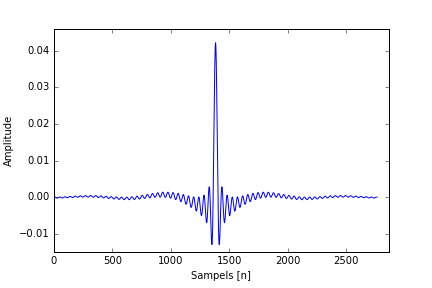
\includegraphics[scale=0.4]{figures/filtertest/impulse.png}
\caption{Impulse response of filter with order $M=2766$}
\label{fig:FIRimpulse}
\end{figure}
       
\begin{figure}[h]
\centering
\begin{subfigure}{0.49\textwidth}
\centering
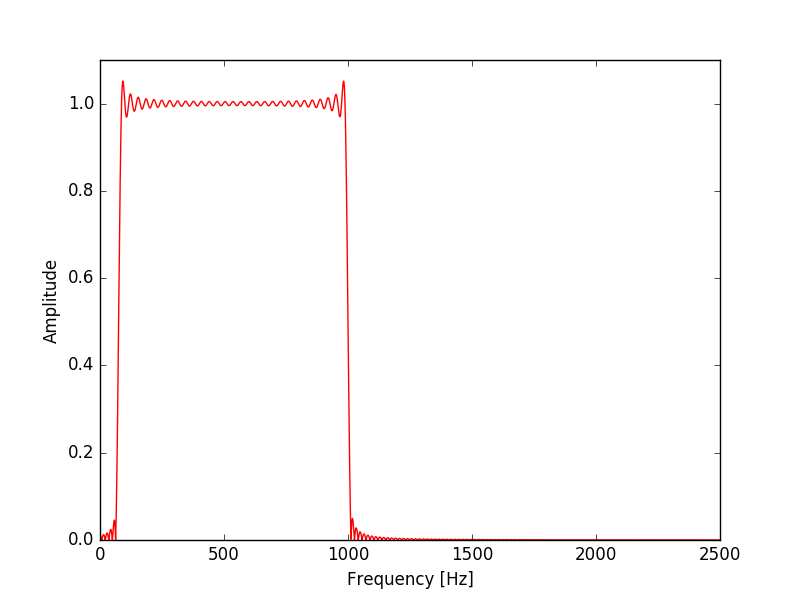
\includegraphics[width=\textwidth]{figures/filtertest/freq_response1.png}
\caption{}
\label{fig:freq_filt1}
\end{subfigure}
\begin{subfigure}{0.49\textwidth}
\centering
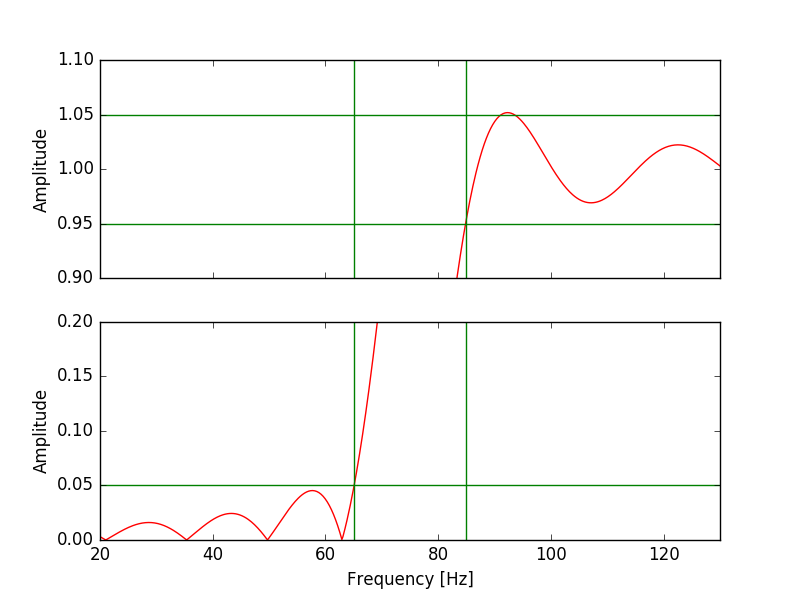
\includegraphics[width=\textwidth]{figures/filtertest/freq_response2.png}
\caption{}
\label{fig:freq_filt2}
\end{subfigure}
\caption{(a) Amplitude response of filter. (b) Close-up view of amplitude response of filter, showing top and bottom of one transitionband.}
\label{fig:freq_filt}
\end{figure}

\begin{algorithm}[H]
\caption{Compute type I FIR filter}
\label{alg:FIR}
\begin{algorithmic}[1] 
\Procedure{Compute kaiser window $w$}{}
\State $A=-20\log_{10}(\delta)$ \Comment{$21 \leq A \leq 50$}
\State $\beta = 0.5824(A-21)^{0.4} + 0.07886(A-21)$ \Comment {Shape parameter}
\State $M = (A-8)/(2.285 \cdot \frac{tw}{f_s} 2\pi)$ \Comment {Filter order, round to upper even int.}
\State $N = M+1$ \Comment {Length of filter}
	\For {each $i$ in length of $N$}
		\For {each $j$ in length of $M$}
			\State $ sum_n + = \ (\frac{1}{j!})^2 \left( \left( \frac{\beta}{2} \sqrt{\left(1 - \left( \frac{2 \cdot i}{N-1}\right) - 1\right)^2}\right)^{2j}\right)$
			\State $ sum_d + = \ (\frac{1}{j!})^2 \left( \frac{\beta}{2}\right)^{2j}$
		\EndFor
		\State $w[i]=\frac{sum_n}{sum_d}$
	\EndFor
	\State Return $w$, $M$
\EndProcedure
\\
\Procedure{Compute ideal impulse response $h_d$}{}
   \For {each $i$ in length of $N$}
        \If {$i == \frac{M}{2}$}
        		\State $h_d[i] = 2( \frac{f_{c2}}{f_s} - \frac{f_{c2}}{f_s})$
        	\Else 
        		\State  $h_d[i] = \frac{1}{ (\pi (i - \frac{M}{2}))}(\sin(\frac{f_{c2}}{f_s} 2 \pi (i - \frac{M}{2})) - (\sin(\frac{f_{c1}}{f_s} 2 \pi (i - \frac{M}{2}))))$ 
          	\EndIf 
  	\EndFor
  	\State Return $h_d$
\EndProcedure
\\
\Procedure{Compute impulse response $h$}{}
	\State Return $h = h_d \cdot w$ \Comment{Windowed impulse response}
\EndProcedure


\end{algorithmic}
\end{algorithm}

\subsection{Test of the filter}
The implemented filter is tested according to the test specifications described in section \ref{sec:testspec}. Figure \ref{fig:SIGNAL} shows the frequency spectrum of the single low E tone with additive noise in form of a beat of hands clapping. Figure \ref{fig:filt_SIGNAL} shows the filtered signal. Note that the frequency spectrum are only showed from 0 to approximately 2200 Hz.  

\begin{figure}[H]
\centering
\begin{subfigure}{0.49\textwidth}
\centering
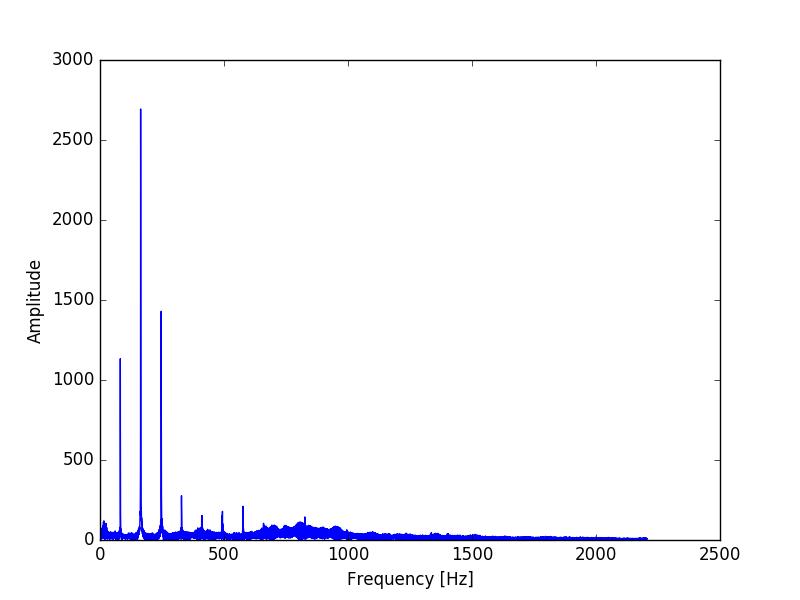
\includegraphics[width=\textwidth]{figures/filtertest/SIGNAL.png}
\caption{}
\label{fig:SIGNAL}
\end{subfigure}
\begin{subfigure}{0.49\textwidth}
\centering
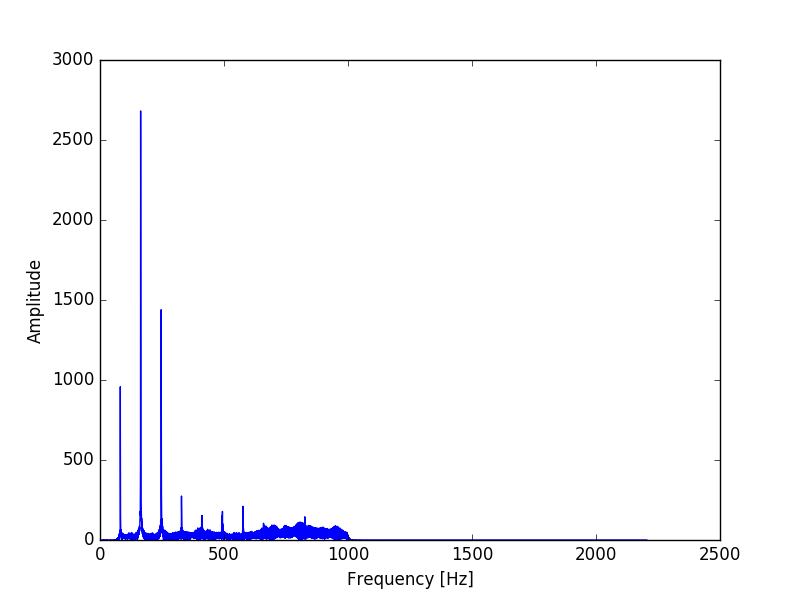
\includegraphics[width=\textwidth]{figures/filtertest/filt_SIGNAL.png}
\caption{}
\label{fig:filt_SIGNAL}
\end{subfigure}
\caption{(a) Frequency spectrum of signal with noise. (b) Frequency spectrum of filtered signal.}
\label{fig:test_res}
\end{figure}
As described in the specifications the filter is designed to remove all frequencies outside the frequencyband from 75 Hz to 1000 Hz. It is seen by comparing figure \ref{fig:SIGNAL} and figure \ref{fig:filt_SIGNAL} that the frequencies outside the passband appears to be zero and that the amplitudes of the remaining frequencies are appropriately the same. \\
By this the designed filter of order 2766 fulfil the specifications and the implementation of the filter works as intended. \\

\section{STFT}

\section{Spectrogram}

\section{Integration validation}

\section{Final system test}


\cleardoublepage
\chapter{Peak detection with varying noise levels} \label{ch11}
In this chapter the peak detection algorithm is tested under varying signal-to-noise ratios. The goal is to investigate the usefulness of the implemented algorithm when the recorded music includes varying levels of noise.
\section{Signal-to-noise ratio}
Signal-to-noise ratio (SNR) is a measure of the amount of noise in a signal. The SNR is defined as
\begin{equation}\label{eq:SNR}
SNR=\frac{\sigma_{signal}^2}{\sigma_{noise}^2}
\end{equation}
where $\sigma_{signal}^2$ is the variance of the wanted signal and $\sigma_{noise}^2$ is the variance of the noise. In this section the recorded music will be added noise in various level such that the SNR is changed. The peak detection algorithm is then used to find peaks, and it is observed when it does not manage to find the right peak as a consequence of the excessive noise in the signal.
\cleardoublepage
\chapter{Wavelet Analysis}
The purpose of this chapter is merely to introduce the concept of wavelet analysis in order to apply it as an alternative to the Fourier transform described and applied in the former chapters.
\\ \\
As described in \ref{ch6}, the STFT is limited by Heisenberg's uncertainty principle. Even though a window with a certain width that satisfies the relation $\sigma_t^2 \sigma_\omega^2 = \frac{1}{4}$ is chosen, the width of the window cannot be changed during the analysis, which means that the Fourier transform is unsuitable to describe signals with both low and high frequencies. The wavelet transform is a different kind of transform, which is used to gain localized information in both frequency and time domains. While the Fourier transform converts a signal between the time and frequency domains, the coefficients of the wavelet transform represent details of the signal at different scale levels and their corresponding temporal location.
\\
This is summarized by figure \martin{Lav figur og indsæt reference. \textregistered}, which shows 4 \textit{Heisenberg boxes}, where the area of each cell in each box are similar. The first box shows the signal in time with full time resolution but no frequency resolution; the second box shows the frequency spectrum achieved by the Fourier transform of the signal with full frequency resolution but no time resolution; the third box shows the STFT of the signal with a fixed window size and with equally (but not arbitrarily) good resolutions in time and frequency; and finally, the fourth box shows the wavelet transform of the signal with varying scale levels and their corresponding time resolution. At a low scale level the window is wide, which gives a good frequency resolution but poor time resolution, and at a high scale level the window is narrow, which conversely gives poor frequency resolution but good time resolution. Furthermore, the area of each cell in the boxes for the STFT and the wavelet transform are determined by the width of the window and the particular wavelet being used, respectively \cite{pages 409-410, Wang} \cite{page 43-44, wave_tut}.

\section{Definition of wavelets}
Wavelet theory provides a way of constructing orthonormal bases in the space $\mathcal{L}^2(\mathbb{R})$. A wavelet system is scaled and translated versions of a fixed function. For an orthonormal basis $\{\textbf{e}_k\}$ of $\mathcal{L}^2(\mathbb{R})$ all functions $f \in \mathcal{L}^2(\mathbb{R})$ have an expansion
\begin{align*}
f = \sum_{k\in\mathbb{Z}}^\infty \langle f, \textbf{e}_k \rangle \textbf{e}_k.
\end{align*}

The index set of the sum is generally infinite but in order for the representation to be of practical use, the functions $f$ must be able to be approximated well by finite partial sums \cite{page 160, FSE2010}.

\begin{definition}[Wavelet]
Let $\psi \in \mathcal{L}^2(\mathbb{R})$.
\begin{enumerate}
\item For $j,k \in \mathbb{Z}$, define the function $\psi_{j,k}$ by
\begin{align*}
\psi_{j,k}(t) = 2^{j/2} \psi(2^jt-k), \quad t \in \mathbb{R}.
\end{align*}
\item The function $\psi$ is called a wavelet if the functions $\{\psi_{j,k}\}_{j,k\in\mathbb{Z}}$ form an orthonormal basis for $\mathcal{L}^2(\mathbb{R})$.
\end{enumerate}
\end{definition}

Therefore, $\psi_{j,k}$ is a dilation and translation as defined in definition \ref{def:TMD} and may be written in terms of the translation operator $T_k$ and the dilation operator $D$ as \cite{page 160, FSE2010}
\begin{align*}
\psi_{j,k} = D^j T_k \psi, \quad j,k \in \mathbb{Z}.
\end{align*}

A simple wavelet is the Haar wavelet.

\begin{definition}[Haar Wavelet] \label{HaarWave}
The \textit{Haar function} is defined by
\begin{align*}
\psi(t) =
\begin{cases}
1 \quad &\textnormal{if } 0 \leq t < \frac{1}{2} \\
-1 \quad &\textnormal{if } \frac{1}{2} \leq t < 1 \\
0 \quad &\textnormal{otherwise}
\end{cases}
\end{align*}
\end{definition}

%The proof that the functions $\{\psi_{j,k}\}_{j,k\in\mathbb{Z}}$ constitute an orthonormal basis for $\mathcal{L}^2$ is quite technical and will therefore be skipped as the purpose of this chapter is merely to introduce and apply wavelet analysis as an alternative to the Fourier transform \cite{page 161, FSE2010} \martin{Overvej dette. \textregistered}.
%\\ \\
The wavelet $\psi(t)$ is usually compactly supported, which means that $\psi(t) \neq 0$ only inside a bounded interval $a < t < b$. Furthermore, $\psi(t) \in \mathcal{L}^1$ has zero mean, which means that it takes both positive and negative values:
\begin{align*}
\int_{-\infty}^\infty \psi(t) dt = 0.
\end{align*}

Therefore, since a wavelet is nonzero only within a finite range and the mean is zero, then $\psi(t)$ has the form of a wave, which is the reason why $\psi(t)$ is called a wavelet \cite{page 411, Wang}. The Haar wavelet is discontinuous at $t = 0, \frac{1}{2}, 1$. Examples of other wavelets that are continuous are the Shannon, Mortlet, and Marr wavelets \cite{page 417-420, Wang}.
\\ \\
The following definition is the background for a main theorem of this section \cite{page 170, FSE2010}.

\begin{definition}[Vanishing moments]
Let $N \in \mathbb{N}$. A function $\psi$ has $N$ vanishing moments if
\begin{align*}
\int_{-\infty}^\infty x^\ell \psi(x) dx = 0 \quad for \quad \ell = 0, 1, \dots, N-1.
\end{align*}
\end{definition}

A relevant wavelet function is the Daubechies' wavelet of degree $N$, which has $N$ vanishing moments and is supported on $[0,2N-1]$. The Haar wavelet defined in definition \ref{HaarWave} is a Daubechies' wavelet of degree $1$ \cite{page 174, FSE2010}. If the wavelet $\psi$ has a large number of vanishing moments, the following result shows that only relatively few coefficients $\langle f, \psi_{j,k} \rangle$ will be large and therefore only a small number of wavelets are needed in the expansion.

\begin{theorem}[Decay of wavelet coefficients]
Assume that the function $\psi \in \mathcal{L}^2(\mathbb{R})$ is compactly supported and has $N$ vanishing moments. Then, for any $N$ times differentiable function $f \in \mathcal{L}^2(\mathbb{R})$ for which the $N$'th derivative $f^{(N)}$ is bounded, there exists a constant $C > 0$ such that
\begin{align} \label{eq:decay_wave_coeff}
|\langle f, \psi_{j,k} \rangle| \leq C 2^{-jN} 2^{-j/2}, \quad \forall \ j \geq 1, \quad k \in \mathbb{Z}.
\end{align}
\end{theorem}

\eqref{eq:decay_wave_coeff} suggests that a high number of vanishing moments $N$ implies that the numbers $\langle f, \psi_{j,k} \rangle$ decay quickly as $j \to \infty$. Therefore, the higher the number of vanishing moments a wavelet has, the fewer coefficients $\{ \langle f, \psi_{j,k} \rangle \}_{j\in\mathbb{N},k\in\mathbb{Z}}$ are needed in the expansion \cite{page 170, FSE2010}.
\\ \\
This fact is widely used in different areas of signal processing. In images, small coefficients signify constant intensities, while large coefficients signify edges. Performing wavelet analysis by using a wavelet with many vanishing moments means that many of the coefficients can be discarded by thresholding, which is an efficient compression \cite{page 174, FSE2010}.
\\ \\
Similarly, noise from audio signals like the ones used in this project may be reduced by removing some of the coefficients \cite{page 175, FSE2010}.
\cleardoublepage

\printbibliography[heading=bibintoc]
\label{bib:mybiblio}
\clearpage
\appendix
\chapter{Fourier Series} \label{appA:Fourierseries}
Periodic functions can be represented as a linear combination of oscillating functions such as sines, cosines or the equivalently complex exponentials.
\\ \\
It can be an advantage to decompose functions as a series or integral of ``simpler'' functions to retrieve information:
\begin{align*}
f(x) = \sum_{n=1}^\infty c_n f_n(x)\text{, or } f(x)= \int_{-\infty}^\infty g(u) h(u,x) du.
\end{align*}

Information from a function $f(x)$ will as an example be stored in the coefficient $\{c_n\}_{n=1}^\infty$ which are easily stored on a computer.
\\ \\
A function $f: \mathbb{R} \to \mathbb{R}$ (or $\mathbb{C}$) is called $2\pi$-periodic if $f(\theta + 2\pi) = f(\theta) \ \forall \ \theta\in\mathbb{R}$. The idea of the Fourier series is using the above information to recreate a $2\pi$-periodic signal. The Fourier series is defined as:
\begin{align*}
f(t) &= \dfrac{a_0}{2} + \sum_{n=1}^\infty(a_n \cos(n t) + b_n \sin(n t))\\
&= \sum_{n=-\infty}^{\infty} c_n \text{e}^{j n t}.
\end{align*}

The second part holds per Euler's formula:
\begin{align*}
\cos(n\theta) &= \dfrac{\text{e}^{j n \theta} + \text{e}^{-j n \theta}}{2}, \\
\sin(n \theta) &= \dfrac{\text{e}^{jn\theta}-\text{e}^{-jn\theta}}{2j}.
\end{align*}

It can be simpler to work with the complex exponential function, but working with the trigonometric functions cosine and sine have their advantages such as being real-valued and also odd and even for the sine and cosine functions, respectively.

\section{The coefficient $c_n$}
The $c_n$ coefficient is determined by the assumption that it is possible to integrate the Fourier series by parts.
\\ \\
To determine $c_n$ in the equation $f(t)= \sum_{n=-\infty}^{\infty} c_n \text{e}^{j n t}$ first multiply both sides by $\text{e}^{-j k t}$ for $k\in \mathbb{Z}$ and integrate both sides from $-\pi$ to $\pi$:
\begin{align} \label{eq:firststep_fouriercoefficient}
\int_{-\pi}^\pi f(t)\text{e}^{-j k t} dt = \int_{-\pi}^\pi \sum_{n=-\infty}^{\infty} c_n \text{e}^{j n t} \text{e}^{-j k t} dt.
\end{align}

Pulling the summation and the constant on the right-hand side out of the integral in \eqref{eq:firststep_fouriercoefficient} yields the following:
\begin{align*}
\int_{-\pi}^\pi f(t) \text{e}^{-j k t}dt = \sum_{n=-\infty}^\infty c_n \int_{-\pi}^\pi \text{e}^{j (n-k) t}dt.
\end{align*}

The integral on the right-hand side has two cases to consider, $n \neq k$ and $n = k$. For $n\neq k$:
\begin{align*}
	\int_{-\pi}^\pi \text{e}^{j(n-k)t}dt 
	=\dfrac{1}{j(n-k)}\text{e}^{j(n-k)t}\mid_{-\pi}^{\pi}
	=\dfrac{(-1)^{n-k}-(-1)^{n-k}}{j(n-k)}
	=0.
\end{align*}

The second case is for $n = k$:
\begin{align*}
\int_{-\pi}^\pi \text{e}^{j(n-k)t}dt = \int_{-\pi}^\pi 1 dt = 2\pi.
\end{align*}

The integral can be concluded to yield either $2\pi$ or $0$:
\begin{align}
	\int_{-\pi}^{\pi} \text{e}^{j (n-k)t}dt 
	= 
	\begin{cases}
			2\pi \text{ if } n=k\\
			0 \text{ otherwise}
	\end{cases}
\end{align}

Therefore, for $n = k$:
\begin{align*}
\int_{-\pi}^\pi f(t)\text{e}^{-j k t} dt = 2\pi c_k.
\end{align*}

Changing the index to $n$ gives the coefficient $c_n$'s general equation:
\begin{align*}
	c_n = \dfrac{1}{2\pi} \int_{-\pi}^{\pi} f(t) \text{e}^{-j n t}dt.
\end{align*}

The above is defined in the following definition \cite{page 18-20, FAA}.

\begin{definition} \label{def:fourier_definition}
The Fourier series of a $2\pi$-periodic integrable function $f(t)$ is defined as:
\begin{align*}
	f(t) = \sum_{n=-\infty}^\infty c_n \text{e}^{j n t},
\end{align*}

where $c_n = \frac{1}{2\pi}\int_{- \pi}^\pi f(t) \text{e}^{-j n t} dt$. Therefore, $c_0 = \frac{a_0}{2} = \frac{1}{2\pi} \int_{-\pi}^\pi f(t) dt$, which is the average of $f$ on the interval $[-\pi,\pi]$.
\\ \\
The Fourier series can alternatively be expressed as:
\begin{align*}
	\dfrac{a_0}{2} + \sum_{n=1}^{\infty} \left[ a_n \cos(n t) + 	b_n \sin(n t)\right],
\end{align*}

where
\begin{align*}
	a_n 
	&= \dfrac{1}{\pi} \int_{-\pi}^\pi f(t) \cos (n t) dt, \quad 	n \geq 0, \\
	b_n
	&= \dfrac{1}{\pi} \int_{-\pi}^\pi f(t) \sin (n t) dt, \quad 	n \geq 1.
\end{align*}
\end{definition}

Since $\cos(nt)$ is even and $\sin(nt)$ is odd, this definition gives the following result \cite{page 21, FAA}.

\begin{lemma}
If $f(t)$ is even, then $f(t)\cos(nt)$ is even and $f(t)\sin(nt)$ is odd, which means that:
\begin{align*}
a_n = \dfrac{2}{\pi} \int_0^\pi f(t) \cos(nt) dt, \quad b_n = 0.
\end{align*}

Likewise, if $f(t)$ is odd, then $f(t)\cos(nt)$ is odd and $f(t)\sin(nt)$ is even, which means that:
\begin{align*}
a_n = 0, \quad b_n = \dfrac{2}{\pi} \int_0^\pi f(t) \sin(nt) dt.
\end{align*}
\end{lemma}

As the following lemma shows, integration of a $2\pi$-periodic function over the length of the period can be shifted to any other interval of length $2\pi$.

\begin{lemma}\label{lemma:2pi-periodic_function}
Suppose $F$ is $2\pi$-periodic and integrable. Then for any real number a:

\begin{align}
\int_a^{2\pi+a}F(t) dt = \int_0^{2\pi}F(t)dt.
\end{align}
\end{lemma}

\begin{proof}
\begin{align*}
	\int_0^{2\pi} F(t)dt 
	&= \int_0^a F(t) dt + \int_a^{2\pi} F(t) dt
	= \int_0^a F(t+2\pi)dt + \int_a^{2\pi} F(t) dt\\ 
	&= \int_{2\pi}^{2\pi + a} F(t) dt + \int_a^{2\pi}F(t)dt
	= \int_a^{2\pi+a}F(t)dt.
\end{align*}
\end{proof}

\section{Convergence of the Fourier series}
In this section the convergence of the Fourier series is examined through piecewise continuous and piecewise smooth functions. The section is inspired by \cite{page 31-36, FAA}.

\begin{definition}
Suppose $-\infty < a < b < \infty$. A function $f$ on $[a,b]$ is piecewise continuous if:
\begin{enumerate}
\item $f$ is continuous on $[a,b]$ except perhaps at finitely many points $x_1, \dots, x_k$.
\item The left-hand and right-hand limits of $f$ at each of the points $x_1, \dots, x_k$ exist:
\begin{align*}
f(x_j-) &= \lim_{h\to 0} f(x_j - h) \\
f(x_j+) &= \lim_{h\to 0} f(x_j + h)
\end{align*}

for $h > 0$. Notice that only the right-hand (or left-hand) limit is required to exist if one of the points $x_j$ is the endpoint $a$ (or $b$).
\end{enumerate}

The space of piecewise continuous functions on $[a,b]$ is denoted as $PC(a,b)$.
\end{definition}

From this definition follows the definition of piecewise smooth functions:
\begin{definition}
The space of piecewise smooth functions on $[a,b]$ is denoted as $PS(a,b)$. $f\in PS(a,b)$ iff
\begin{enumerate}
	\item $f \in PC(a,b)$.
	\item $f'$ exists and is also piecewise continuous on $[a,b]$. This means that $f'$ is continuous except perhaps at finitely many points $x_1, \dots, x_K$ (which includes the points where $f$ is discontinuous), and that the limits $f'(x_j-)$, $f'(x_j+)$, $f'(a+)$ and $f'(b-)$ exist (for $j = 1,\dots, K$).
\end{enumerate}
\end{definition}

To sum up, $f$ is piecewise smooth if its graph only has finitely many jumps and corners where $f$ and $f'$ are discontinuous, respectively. E.g. $f(x) = \frac{1}{x}$ at $x = 0$ and sharp cusps results in infinite discontinuities for $f$ and $f'$, respectively, and are not allowed for piecewise smooth functions.
\\ \\
For a $2\pi$-periodic and integrable function, the $N$'th partial sum of the Fourier series is defined by:
\begin{align}\label{eq:partialsumFourierSeries}
	S_N^f(t) = \dfrac{1}{2} a_0 + \sum_{n=1}^N\left(a_n \cos(n 		t) + b_n \sin(n t) \right) = \sum_{n=-N}^N c_n \text{e}^{j n t}
\end{align}

with the coefficients $a_n$, $b_n$ and $c_n$ as in definition \ref{def:fourier_definition}.
\\ \\
Inserting $c_n$ in the partial sum using $x$ in place of the variable $t$ in definition \ref{def:fourier_definition} yields:
\begin{align*}
	S_N^f(t)
	&= \dfrac{1}{2\pi}\sum_{n=-N}^N \int_{-\pi}^\pi f(x) 			\text{e}^{-j n x} dx\, \text{e}^{j n t} \\
	&= \dfrac{1}{2\pi}\sum_{k = -N}^N \int_{-\pi}^\pi f(x) 			\text{e}^{j k (x-t)} dx, \quad \quad k = -n, \\
	&= \dfrac{1}{2\pi} \sum_{n = -N}^N \int_{-\pi - t}^{\pi - 		t} f(t + \tau ) \text{e}^{j n \tau} d\tau, \quad \quad \tau 	= x-t.
\end{align*}

By lemma \ref{lemma:2pi-periodic_function} the above equation can be expressed as follows
\begin{align} \label{eq:dirichlet}
	S_N^f (t) 
	&= \dfrac{1}{2\pi} \sum_{n=-N}^N \int_{-\pi}^\pi f(t + 			\tau) \text{e}^{j n \tau} d\tau \nonumber \\
	&= \int_{-\pi}^\pi f(t + \tau) D_N(\tau) d\tau,
\end{align}

where $D_N(\tau) = \dfrac{1}{2\pi}\sum_{n=-N}^{N}\text{e}^{j n \tau}$ is called the $N$'th Dirichlet kernel. The following lemma is inspired by \cite{page 30, FAA}.

\begin{lemma}[Bessel's Inequality] \label{lemma:Bessel1}
If $f$ is $2\pi$-periodic and Riemann integrable on $[-\pi,\pi]$, and the Fourier coefficients $c_n$ as defined in definition \ref{def:fourier_definition}, then
\begin{align*}
\sum_{n=-\infty}^\infty |c_n|^2 \leq \dfrac{1}{2\pi} \int_{-\pi}^\pi |f(t)|^2 dt.
\end{align*}
\end{lemma}

\begin{proof}
For $z \in \mathbb{C}$ then $|z|^2 = z \overline{z}$. For $N \in \mathbb{N}$
\begin{align*}
0 &\leq \left| f(t) - \sum_{n=-N}^N c_n \text{e}^{jnt} \right|^2 = \left( f(t) - \sum_{n=-N}^N c_n \text{e}^{jnt} \right) \left( \overline{f(t)} - \sum_{n=-N}^N \overline{c_n} \text{e}^{-jnt} \right) \\
&= |f(t)|^2 - \sum_{n=-N}^N \left[ c_n \overline{f(t)} \text{e}^{jnt} + \overline{c_n} f(t) \text{e}^{-jnt} \right] + \sum_{m,n=-N}^N c_m\overline{c_n} \text{e}^{j(m-n)t}.
\end{align*}

Multiplying both sides by $\frac{1}{2\pi}$ and integrating from $-\pi$ to $\pi$ gives
\begin{align*}
0 &\leq \dfrac{1}{2\pi} \int_{-\pi}^\pi \left| f(t) - \sum_{n=-N}^N c_n \text{e}^{jnt} \right|^2 dt = \dfrac{1}{2\pi} \int_{-\pi}^\pi |f(t)|^2 dt - \sum_{n=-N}^N \left[ c_n \overline{c_n} + \overline{c_n} c_n \right] + \sum_{n=-N}^N c_n \overline{c_n} \\
&= \dfrac{1}{2\pi} \int_{-\pi}^\pi |f(t)|^2 dt - \sum_{n=-N}^N |c_n|^2
\end{align*}

since
\begin{align*}
\dfrac{1}{2\pi} \int_{-\pi}^\pi \text{e}^{j(m-n)t} dt =
\begin{cases}
1, \ m = n \\
0, \ m \neq n
\end{cases}
\end{align*}

It follows that
\begin{align*}
\sum_{n=-N}^N |c_n|^2 \leq \dfrac{1}{2\pi} \int_{-\pi}^\pi |f(t)|^2 dt.
\end{align*}

Letting $N\to\infty$ completes the proof.
\end{proof}

The following corollary is used to prove theorem \ref{theo:main_convergence} \cite{page 31, FAA}.

\begin{corollary} \label{coro:conv_Fourier_coeff}
The Fourier coefficients $a_n$, $b_n$ and $c_n$ all tend to zero as $n \to \pm \infty$.
\end{corollary}

The following theorem is the main convergence theorem in this section \cite{page 35, FAA}.

\begin{theorem} \label{theo:main_convergence}
Let $f(t)$ be $2\pi$-periodic and piecewise smooth on $\mathbb{R}$. Then the limit of the partial sum $S_N^f$ is
	\begin{align*}
		\lim_{N\to\infty} S_N^f (t) = \dfrac{1}{2}\left[f(t-) + 		f(t+)\right], \, t \in [-\pi, \pi].
	\end{align*}

If $f$ is continuous at $t$, then
	\begin{align*}
		\lim_{N\to \infty} S_N^f(t) = f(t).
	\end{align*}
\end{theorem}

\begin{proof}
The integral from $-\pi$ to $0$ and from $0$ to $\pi$ of a Dirichlet kernel both equals $\frac{1}{2}$ \cite{page 35, FAA}. Hence:
	\begin{align*}
		\dfrac{1}{2} f(\theta-) = f(\theta-) \int_{-\pi}^0 				D_N(\tau)d\tau, \quad \dfrac{1}{2}f(\theta+) = 					f(\theta+) \int_0^\pi D_N (\tau)d\tau,
	\end{align*}
	
	which by \eqref{eq:dirichlet} gives:
	\begin{align} \label{eq:S_N_proof}
		S_N^f(\theta) &- \dfrac{1}{2}\left[f(\theta-) + 				f(\theta+)\right] \nonumber \\
		&= \int_{-\pi}^0 \left[f(\theta + \tau) - f(\theta-) 			\right] D_N(\tau) d\tau + \int_0^\pi \left[f(\theta + 			\tau) - f(\theta+) \right] D_N(\tau) d\tau.
	\end{align}
	
	The $N$'th Dirichlet kernel may be written as:
	\begin{align} \label{eq:Dirichlet_proof}
		D_N(\tau) &= \dfrac{1}{2\pi}\sum_{n=-N}^{N}\text{e}^{j 			n \tau} = \dfrac{1}{2\pi} \text{e}^{-jN\tau} \sum_{n=0}			^{2N} \text{e}^{jn \tau} \nonumber \\
		&= \dfrac{1}{2\pi} \text{e}^{-jN\tau} \dfrac{e^{j(2N+1)			\tau}-1}{\text{e}^{j\tau}-1} = \dfrac{1}{2\pi} 					\dfrac{\text{e}^{j(N+1)\tau}-\text{e}^{-jN\tau}}				{\text{e}^{j\tau}-1}, \quad \tau \neq 0
	\end{align}
	
	since in general:
	\begin{align*}
		\sum_{n=0}^K r^n = \frac{r^{K+1}-1}{r-1}, \quad r \neq 			1.
	\end{align*}
	
	A function $g(\tau)$ is defined to be:
	\begin{align} \label{eq:g_tau}
		g(\tau) =
		\begin{cases}
			\dfrac{f(\theta + \tau) - f(\theta-)}{\text{e}^{j				\tau}-1} \quad \text{for } -\pi < \tau < 0 \\ \\
			\dfrac{f(\theta + \tau) - f(\theta+)}{\text{e}^{j				\tau}-1} \quad \text{for } 0 < \tau < \pi
		\end{cases}
	\end{align}	
	
	By using \eqref{eq:Dirichlet_proof} and \eqref{eq:g_tau}, 		then \eqref{eq:S_N_proof} may be written as the Fourier 		coefficients:
	\begin{align} \label{eq:5.1.1_final}
		\dfrac{1}{2\pi} \int_{-\pi}^\pi g(\tau) \left(\text{e}			^{j(N+1)\tau} - \text{e}^{-jN\tau}\right) d\tau = C_{-			(N+1)} - C_N.
	\end{align}
	
	$g$ is a well-behaved function on $[-\pi,\pi]$ except near 		$\tau = 0$ where the denominator equals 0, which suggests 		that $g$ is not piecewise continuous. However, by 				l'Hôpital's rule:
	\begin{align*}
		\lim_{\tau \to 0+} g(\tau) = \lim_{\tau \to 0+} 				\dfrac{f(\theta + \tau) - f(\theta+)}{\text{e}^{j				\tau}-1} = \lim_{\tau \to 0+} \dfrac{f'(\theta + \tau)}			{j\text{e}^{j\tau}} = \dfrac{f'(\theta+)}{j}.
	\end{align*}
	
	Likewise, $\displaystyle{\lim_{\tau \to 0-}} g(\tau) = 			\frac{f'(\theta-)}{j}$. Both of these limits are finite, 		and hence $g$ is actually piecewise continuous on $[-\pi,		\pi]$. The Fourier coefficients $C_N = \frac{1}{2\pi} 			\int_{-\pi}^\pi g(\tau)\text{e}^{-jN\tau} d\tau$ tend to 		zero as $N 	\to \pm \infty$ by corollary 						\ref{coro:conv_Fourier_coeff}. 	Therefore,
	\eqref{eq:5.1.1_final} also vanishes as $N \to \infty$, 		which shows that \eqref{eq:S_N_proof} also tend to zero as 		$N \to \infty$, which completes the proof.
\end{proof}

\section{Orthogonality of the Fourier Series} \label{sec:FS_ort}
According to \cite{page 62, FAA}, Fourier series are one of a large class of interesting and useful infinite series expansions that are based on so-called \textit{orthogonal systems} or \textit{orthogonal sets} of functions.\\
This section studies the orthogonality of the Fourier series and is inspired by \cite{pages 62-77, FAA} and the lecture notes from the course \textit{Anvendt Harmonisk Analyse}.
For $\textbf{x},\textbf{y} \in \mathbb{C}^N$ the dot product is
\begin{align*}
\langle \textbf{x},\textbf{y} \rangle = \sum_{i=1}^N x_i \overline{y_i},
\end{align*}

and the vectors $\textbf{x},\textbf{y}$ are said to be orthogonal if $\langle \textbf{x},\textbf{y} \rangle = 0$. The norm on $\mathbb{C}^N$ is:
\begin{align*}
\|\textbf{x}\|^2 = \langle \textbf{x},\textbf{x} \rangle
\end{align*}

A basis $\{\textbf{b}_\textbf{j}\}_{j=1}^N$ is an orthonormal basis for $\mathbb{C}^N$ if it is orthogonal and normalized:
\begin{align*}
\langle \textbf{b}_\textbf{i}, \textbf{b}_\textbf{j} \rangle =
\begin{cases}
	1, \ i = j \\
	0, \ i \neq j
\end{cases}
\end{align*}

The decomposition of a vector $\textbf{x} \in \mathbb{C}^N$ is:
\begin{align*}
\textbf{x} = \sum_{i=1}^N \langle \textbf{x}, \textbf{b}_\textbf{i} \rangle \textbf{b}_\textbf{i}.
\end{align*}

The Fourier series fits into this theory formation. For
$f,g \in PC(a,b)$ the inner product and norm is defined as
\begin{align*}
\langle f,g \rangle = \int_a^b f(x) \overline{g(x)} dx,
\|f\| = \left( \int_a^b |f(x)|^2 dx \right)^{\frac{1}{2}} = \sqrt{\langle f,f \rangle}.
\end{align*}

Furthermore, for $f,g \in PC(a,b)$, the Cauchy-Schwarz inequality and the triangle inequality holds for all norms an inner products:
\begin{align*}
|\langle f,g \rangle| &\leq \|f\| \|g\|, \\
\|f+g\| &\leq \|f\| + \|g\|.
\end{align*}

Consider the function $\phi(t) = \frac{1}{\sqrt{2\pi}} \text{e}^{jnt}$ defined on $[-\pi,\pi]$. Since
\begin{align*}
\langle \phi_m, \phi_n \rangle = \dfrac{1}{2\pi} \int_{-\pi}^\pi \text{e}^{j(m-n)t} dt =
\begin{cases}
1, \ m = n \\
0, \ m \neq n
\end{cases}
\end{align*}

$\{\phi_n\}_{n\in\mathbb{Z}}$ is an orthonormal family of functions. The Fourier coefficient $c_n$ is
\begin{align*}
c_n = \dfrac{1}{2\pi} \int_{-\pi}^\pi f(t) \overline{\text{e}^{jnt}} dt = \dfrac{1}{\sqrt{2\pi}} \langle f,\phi_n \rangle.
\end{align*}

Therefore, the Fourier series for $f$ is
\begin{align} \label{eq:ort_fam}
f(t) = \sum_{n=-\infty}^\infty c_n \text{e}^{jnt} = \sum_{n=-\infty}^\infty \langle f, \phi_n \rangle \phi_n,
\end{align}

which is the decomposition of a vector in $\mathbb{C}^N$ with an orthonormal basis.
\\ \\
For a sequence $\{f_n\}_{n=1}^\infty \in PC(a,b)$ it is said that $f_n \to f$ in norm if
\begin{align*}
\|f - f_n\| = \left( \int_a^b |f(x) - f_n(x)|^2  dx \right)^\frac{1}{2} \to 0 \ \text{for} \ n \to \infty.
\end{align*}

However, $PC(a,b)$ is not complete, which means that there exists a Cauchy-sequence in $PC(a,b)$ that does not converge to a $f \in PC(a,b)$. This problem is solved by imposing the completion $\mathcal{L}^2(a,b)$ (from chapter \ref{ch5}) of $PC(a,b)$ under the norm $\|\cdot\|$:
\begin{align*}
\mathcal{L}^2(a,b) = \{f: \int_a^b |f(t)|^2 dt < \infty \},
\end{align*}

where the integral is the Lebesgue integral. In order to make $\|\cdot\|$ into a norm, equivalence classes of functions are imposed by$^[$\footnote{Further details of these equivalence classes are beyond the scope of this project.}$^]$
\begin{align*}
f \sim g \Leftrightarrow \int_a^b |f(x) - g(x)|^2 dx = 0.
\end{align*}

This is the reason why $\mathcal{L}^2(a,b)$ is a Hilbert space (see also chapter \ref{ch5}). For $f \in \mathcal{L}^2(a,b)$ it is possible to find a sequence of continuous functions $\{f_n\}_{n=1}^\infty$ such that $\|f - f_n\| \to 0$ for $n \to \infty$, where $\{f_n\}$ can be chosen to be a sequence of smooth functions.
\\ \\
The following lemma is a generalization of the special case of Bessel's inequality in lemma \ref{lemma:Bessel1} \cite{page 75, FAA}.

\begin{lemma}[Bessel's inequality] \label{lemma:Bessel2}
Let $\{\phi_n\}_{n=1}^\infty$ be an orthonormal family in $\mathcal{L}^2(a,b)$, and let $f \in \mathcal{L}^2(a,b)$. Then
\begin{align*}
\sum_{n=1}^\infty |\langle f,\phi_n\rangle|^2 \leq \|f\|^2.
\end{align*}
\end{lemma}

\begin{proof}
Since
\begin{align*}
\langle f, \langle f,\phi_n \rangle \phi_n \rangle = \overline{\langle f,\phi_n \rangle} \langle f,\phi_n \rangle = |\langle f, \phi_n \rangle|^2,
\end{align*}

and due to Pythagora's theorem it is seen that
\begin{align*}
\left\|\sum_{n=1}^N \langle f, \phi_n \rangle \phi_n \right\|^2 = \sum_{n=1}^N |\langle f, \phi_n \rangle |^2.
\end{align*}

Since $\|a + b\|^2 = \|a\|^2 + 2 \operatorname{Re} \langle a,b  \rangle + \|b\|^2$ for any $a,b \in \mathbb{C}^k$ \cite{page 64, FAA} it follows that:
\begin{align*}
0 &\leq \|f - \sum_{n=1}^N \langle f, \phi_n \rangle \phi_n\|^2 = \|f\|^2 - 2\operatorname{Re} \left\langle f, \sum_{n=1}^N \langle f,\phi_n\rangle \phi_n \right\rangle + \left\|\sum_{n=1}^N \langle f, \phi_n \rangle \phi_n \right\|^2 \\
&= \|f\|^2 - 2\sum_{n=1}^N |\langle f, \phi_n \rangle |^2 + \sum_{n=1}^N |\langle f, \phi_n \rangle |^2 = \|f\|^2 - \sum_{n=1}^N |\langle f, \phi_n \rangle |^2.
\end{align*}
\end{proof}

This result entails the following lemma.
\begin{lemma}
For $f \in \mathcal{L}^2(a,b)$ and an orthonormal family $\{\phi_n\}_{n=1}^\infty$ the sum $\sum_{n=1}^\infty \langle f,\phi_n \rangle \phi_n$ converges in norm and $\left\| \sum_{n=1}^\infty \langle f,\phi_n \rangle \phi_n \right\| \leq \|f\|$.
\end{lemma}

\begin{proof}
According to Bessel's inequality the sum $\sum_{n=1}^\infty | \langle f,\phi_n \rangle |^2$ converges, which means that
\begin{align*}
\left\|\sum_{n=M}^N \langle f, \phi_n \rangle \phi_n \right\|^2 = \sum_{n=M}^N |\langle f, \phi_n \rangle |^2 \to 0 \ \text{for} \ M,N \to \infty,
\end{align*}

where the equality follows from Pythagora's theorem. Therefore, $\left\{ \sum_{n=1}^N \langle f,\phi_n \rangle \phi_n \right\}_{N=1}^\infty$ is a Cauchy-sequence in the complete space $\mathcal{L}^2(a,b)$, which means that the sequence converges in $\mathcal{L}^2(a,b)$. Furthermore:
\begin{align*}
\left\|\sum_{n=1}^\infty \langle f, \phi_n \rangle \phi_n \right\|^2 = \lim_{N\to \infty} \left\|\sum_{n=1}^N \langle f, \phi_n \rangle \phi_n \right\|^2 = \lim_{N\to\infty} \sum_{n=1}^N | \langle f,\phi_n \rangle |^2 = \sum_{n=1}^\infty | \langle f,\phi_n \rangle |^2 \leq \|f\|^2.
\end{align*}
\end{proof}

The final question in this section is when an orthonormal family in $\mathcal{L}^2(a,b)$ actually is an orthonormal basis for $\mathcal{L}^2(a,b)$. An orthonormal basis $\{\phi_n\}_{n=1}^\infty$ satisfies $f = \sum_{n=-\infty}^\infty \langle f, \phi_n \rangle \phi_n \ \forall f \in \mathcal{L}^2(a,b)$ as in \eqref{eq:ort_fam}. The following theorem is inspired by \cite{page 77, FAA}.

\begin{theorem} \label{theo:Fourier_series_Parseval}
Let $\{\phi_n\}_{n=1}^\infty$ be an orthonormal family in $\mathcal{L}^2(a,b)$. The following conditions are equivalent.
\begin{enumerate}[label=(\alph*)]
\item If $\langle f, \phi_n \rangle = 0$ for all $n$, then $f = 0$.
\item For every $f \in \mathcal{L}^2(a,b)$ we have $f = \sum_{n=1}^\infty \langle f, \phi_n \rangle \phi_n$ with convergence in norm.\\
\item For all $f \in \mathcal{L}^2(a,b)$:
\begin{align*}
\|f\|^2 = \sum_{n=1}^\infty |\langle f,\phi_n \rangle|^2
\end{align*}
This is known as Parseval's equation.
\end{enumerate}
\end{theorem}

\begin{proof}
The proof is recursive, which means that it is proven that condition \textit{(a)} implies \textit{(b)}, which implies \textit{(c)}, which in turn implies \textit{(a)}. In order to prove that \textit{(a)} implies \textit{(b)} let $f\in\mathcal{L}^2(a,b)$. The sum $\sum_{n=1}^\infty \langle f,\phi_n \rangle \phi_n$ converges in norm. Let $g = f - \sum_{n=1}^\infty \langle f,\phi_n \rangle \phi_n$. It follows that
\begin{align*}
\langle g,\phi_m \rangle = \langle f, \phi_m \rangle - \left\langle \sum_{n=1}^\infty \langle f,\phi_n\rangle \phi_n, \phi_m \right\rangle &= \langle f, \phi_m \rangle - \langle f, \phi_m \rangle \\
&= 0 \ \forall \ m \Rightarrow g = 0 \Rightarrow f = \sum_{n=1}^\infty \langle f,\phi_n \rangle \phi_n.
\end{align*}

\textit{(b)} implies \textit{(c)} due to Pythagora's theorem:
\begin{align*}
\|f\|^2 = \lim_{N\to\infty} \left\| \sum_{n=1}^N \langle f,\phi_n \rangle \phi_n \right\|^2 = \lim_{N\to\infty} \sum_{n=1}^N |\langle f,\phi_n \rangle|^2 = \sum_{n=1}^\infty |\langle f,\phi_n \rangle|^2.
\end{align*}

Finally, \textit{(c)} implies \textit{(a)} since if $\langle f,\phi_n \rangle = 0 \ \forall \ n$, then $\|f\| = 0 \Rightarrow f = 0$.
\end{proof}

%http://cnx.org/contents/8YnJdzjg@8/Derivation-of-Fourier-Coeffici

%Note to self foldning.

\clearpage
\chapter{Recordings} \label{recordings}
In this appendix the procedure of the recording of music and noise in an anechoic room is described.

\section{Description}  
The purpose of the recordings are to obtain several different audio files of music to use for both unit tests and tests on the final system. \\
It is important to know the exact signal on each audio files in order to use it as reference when validating the system. Hence recording of the audio will take place in the anechoic room provided by the acoustic laboratory at AAU. \\
Musical signals and noise is recorded separately. Hereby specific noise can be added to the music digitally in order to gain further control of the signals. \\
Table \ref{tab:audio} makes a list representing the contents of each audio file to be recorded. The contents of the musical audio files is selected on behalf of the complexity of the frequencies - from a single note to a melody played with chords.  \\
Each type of file will be recorded at least two times. This is done to verify the note played and minimize the human mistakes.    \\
The noise to be recorded is chosen to represent additive noise that could appear naturally in a situation where the final system would be used. Note that convolution noise is disregarded as a result of recording in the anechoic room.         
\begin{table}[H]
\centering
\caption{List of recordings in the anechoic room.}
\label{tab:audio}
\begin{tabular}{l|l|l}
\hline
  & \textbf{Music}                      & \textbf{Noise}     \\ \hline
1 & Low E string - long/short           & Random speak       \\ \hline
2 & High E string - long/short          & Curling paper      \\ \hline
3 & Low E chord                         & Random clapping    \\ \hline
4 & High E chord                        & Rhythmical clapping \\ \hline
5 & Melody of single strings - slow/fast & Random cheering    \\ \hline
6 & Melody with chords - slow/fast      & Singing            \\ \hline
\end{tabular}
\end{table}
Beside the listed audio files, which add up to $15$ different files, natural outdoor sound is also recorded outside the anechoic room. 

\subsection{Anechoic room} 
An anechoic room is designed to absorb all reflections from sound or electromagnetic waves. Further the room is isolated from exterior noise, which makes it possible to only record or measure the exact sound that is coming from the instrument without the presence of interfering reflections. \\ The specific room at AAU is build as a box inside a box. The inner box is placed on rubber suspensions, and the inner walls are covered by sound absorbing wedges of about 0.4 m length due to requirements for anechoic performances. The inside dimensions of the room are 4.5 m times 5.0 m with a height of 4.0 m.\cite{anechoic}.\\
Hence, by recording in the anechoic room signal noise is reduced to a minimum.

\section{Procedure}
\textbf{Set up for inside anechoic room:}\\
\begin{itemize}
\item[-] A grid just big enough to support a microphone stand is install as the only floor in the anechoic room, partly covered by wadding. 
\item[-] One man with Guitar sits on the grid, playing into the microphone. 
- microphone is connected through the wall into the listening/control room besides the anechoic room. 
\end{itemize}   
\textbf{Set up in control room: }
\begin{itemize}
\item[-] Microphone is connected to the ACD, which is connected to the PC.
\item[-] The PC is running the recording program Audacity. From the program the sampling frequency is specified to 44.1 kHz.     
\end{itemize}

Table \ref{tab:equip} specifies the equipment used for the recording. Figures \ref{fig:setup1} and \ref{fig:setup2} show the set up inside the anechoic room.
\begin{table}[H]
\centering
\caption{Equipment list.}
\label{tab:equip}
\begin{tabular}{l|l|l}
\hline
  & \textbf{Equipment}                & \textbf{Specifications}                                                                                      \\ \hline
1 & Condenser Microphone, C 414 B-ULS &                                                                                                              \\ \hline
2 & ADC, Roland Quad-capture          & \begin{tabular}[c]{@{}l@{}}Analog $2 \times 2$, digital $2 \times 2$, USB 2.0,\\ 4 in/4 out, 24 bit , 192 kHz\end{tabular} \\ \hline
3 & PC                                &                                                                                                              \\ \hline
4 & Audacity                          &                                                                                                              \\ \hline
5 & Guitar   	                      &                                                                                                              \\ \hline
6 & Paper   	                      &                                                                                                              \\ \hline
\end{tabular}
\end{table}

\begin{figure}[H]
\centering
	\begin{minipage}{0.49\textwidth}
  	  
    		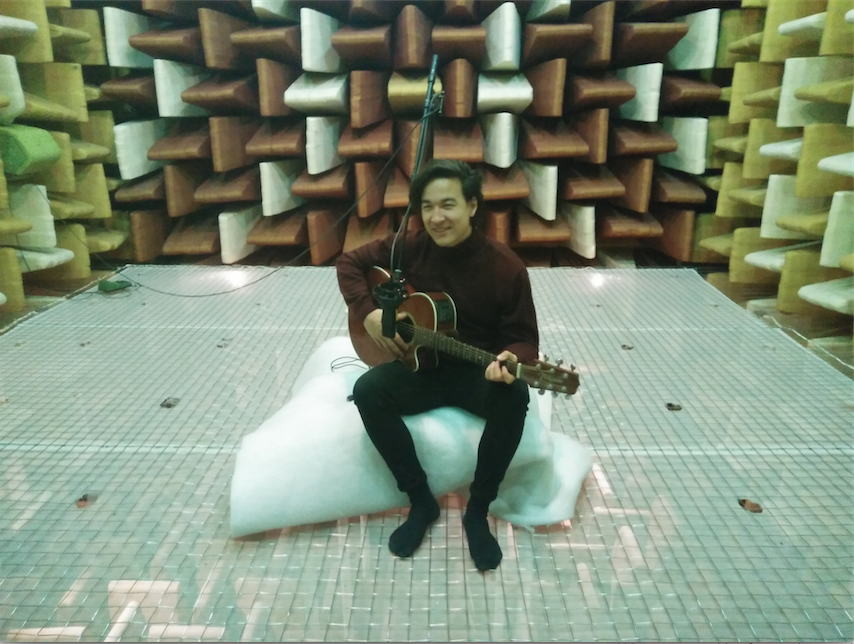
\includegraphics[scale=0.22]{figures/recording/setup1.png}
    		\caption{Set up inside anechoic room.}
    		\label{fig:setup1}
    \end{minipage}
    \begin{minipage}{0.49\textwidth}
  	  
    		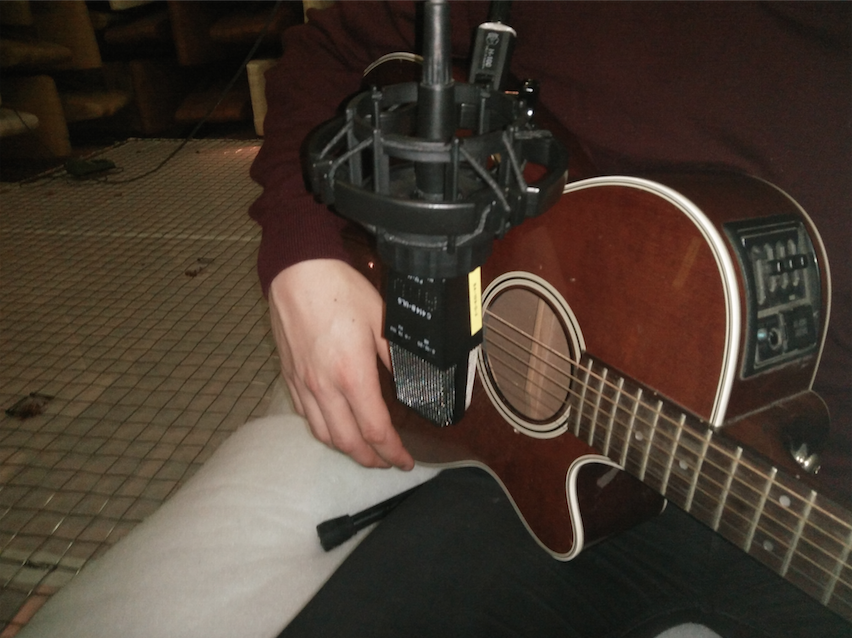
\includegraphics[scale=0.22]{figures/recording/setup2.png}
    		\caption{Set up inside anechoic room.}
    		\label{fig:setup2}
    \end{minipage}
\end{figure} 

\textbf{Recording procedure}\\
Through a communication system the guitar player is told what and when to play by the person controlling Audacity in the control room, who starts and stops the recordings. \\
The procedure for recording the noise follows the same procedure.\\
\\
When recoding the outdoor noise the microphone stand is placed in an open window inside the control room. One long record is taken, which include bird song, car noise, and especially noise from a ventilator. One more more record is made similarly but with low random talking.

\section{Source of errors}
\begin{itemize}
\item[-] Internal noise from microphone will appear. 
\item[-] Minimal reflection of sound signal caused by the floor and the man necessary in the room can occur. 
\item[-] Not playing exactly the note we want to play can make as an error source to consider when validating the final system.
\item[-] The sensibility/gain adjustments to be made on the ADC was adjusted for the recorded sound to not peak within the frequency band provided by Audacity. If a peak is reached without it will cause a an error.            
\end{itemize}

\section{Evaluation}
Usable audio files with minimal amount of noise was obtained from the recording. The noise was minimized by using the anechoic room and further minimizing the amount of equipment and  people in the room.       
A frequency analysis of the recorded signals is described in chapter \ref{ch9}.  


\chapter{Additional material for FIR filter}

\section{Derivation of ideal impulse response}\label{appC}
In order to derive the ideal impulse response for the bandpass filter described in chapter \ref{ch10} the ideal frequency response is defined as follows on behalf of figure \ref{fig:spec_Hd}:
%\begin{align*}
% H_d(\text{e}^{j\omega}) = \begin{cases}
% 0, \ \ \ & |\omega| \leq \omega_{c_1} \\
%  \text{e}^{-j\omega\frac{M}{2}}, \ \ \ & \omega_{c_1} \leq | \omega | \leq \omega_{c_2} \\
%  0, \ \ \ & \omega_{c_2} \leq |\omega| \leq \pi 
%\end{cases}
%\end{align*}

\begin{align*}
H_d(\text{e}^{j\omega}) = \begin{cases}
\text{e}^{-j\omega\frac{M}{2}}, \quad &\begin{cases}
-\omega_{c_2} \leq \omega \leq -\omega_{c_1} \\
\omega_{c_1} \leq \omega \leq \omega_{c_2}
\end{cases} \\
0, \quad &Otherwise
\end{cases}
\end{align*}

From this the ideal impulse response is determined by the inverse Fourier transformation described in definition \ref{def:InverseFourier_trans}:
\begin{align*}
h_d[n] &= \dfrac{1}{2\pi} \int_{-\pi}^\pi H_d(\text{e}^{j\omega}) \text{e}^{j\omega n} d\omega = \dfrac{1}{2\pi} \left(  \int_{-\omega_{c_2}}^{-\omega_{c_1}} \text{e}^{-j\omega \frac{M}{2}} \cdot \text{e}^{j \omega n} d\omega + \int_{\omega_{c_1}}^{\omega_{c_2}} \text{e}^{-j\omega \frac{M}{2}} \cdot \text{e}^{j \omega n} d\omega \right) \\
&= \frac{1}{2\pi} \left( \int_{-\omega_{c_2}}^{-\omega_{c_1}} \text{e}^{j\omega \left(n - \frac{M}{2} \right) } d\omega + \int_{\omega_{c_1}}^{\omega_{c_2}} \text{e}^{j\omega \left(n- \frac{M}{2} \right)} d\omega \right).
\end{align*}

Euler's formula says that $\text{e}^{j\omega t} = \cos(\omega t) + j\sin(\omega t)$. For the first integral above it follows that
\begin{align*}
\int_{-\omega_{c_2}}^{-\omega_{c_1}} \text{e}^{j\omega \left(n- \frac{M}{2} \right)} d\omega &= \int_{-\omega_{c_2}}^{-\omega_{c_1}} \cos \left( \omega \left(n-\dfrac{M}{2}\right)\right) + j \sin \left( \omega \left(n-\dfrac{M}{2}\right) \right) d\omega \\
&= \left[ \sin\left(\omega \left(n-\dfrac{M}{2}\right)\right) \right]_{\omega=-\omega_{c_2}}^{-\omega_{c_1}} \cdot \dfrac{1}{n - \frac{M}{2}}
\end{align*}

since the integral of the second term evaluates to 0. Since $\sin(-\omega\cdot t) = - \sin(\omega \cdot t)$ the impulse response may be written as
\begin{align*}
h_d[n] &= \dfrac{1}{2\pi} \left( \dfrac{1}{n - \frac{M}{2}} \left( \sin \left( - \omega_{c_1} \left( n - \frac{M}{2} \right) \right) - \sin \left( - \omega_{c_2} \left( n - \frac{M}{2} \right) \right) + \sin \left( \omega_{c_2} \left( n - \frac{M}{2} \right) \right) - \sin \left( \omega_{c_1} \left( n - \frac{M}{2} \right) \right) \right) \right) \\
&= \dfrac{1}{2\pi} \left( \dfrac{1}{n - \frac{M}{2}} \left( - \sin \left( \omega_{c_1} \left( n - \frac{M}{2} \right) \right) + \sin \left( \omega_{c_2} \left( n - \frac{M}{2} \right) \right) + \sin \left( \omega_{c_2} \left( n - \frac{M}{2} \right) \right) - \sin \left( \omega_{c_1} \left( n - \frac{M}{2} \right) \right) \right) \right) \\
&= \dfrac{1}{2\pi} \left( \dfrac{2}{n - \frac{M}{2}} \left( - \sin \left( \omega_{c_1} \left( n - \frac{M}{2} \right) \right) + \sin \left( \omega_{c_2} \left( n - \frac{M}{2} \right) \right) \right) \right) \\
&= \dfrac{1}{\pi \left( n - \frac{M}{2}\right)} \left( \sin\left( \omega_{c_2} \left( n - \frac{M}{2} \right) \right) - \sin \left( \omega_{c_1} \left( n - \frac{M}{2} \right) \right) \right).
\end{align*}

This is only true for $n \neq \frac{M}{2}$, and $h_d[M/2]$ must be defined separately. In order to do so l'Hôspital's rule$^[$\footnote{A more detailed version of l'Hôpital's rule may be found at \url{http://tutorial.math.lamar.edu/Classes/CalcI/LHospitalsRule.aspx}.}$^]$, which says that $\lim \frac{f(x)}{g(x)} = \lim \frac{f'(x)}{g'(x)}$, is used. Thus:
\begin{align*}
h_d[M/2] &= \dfrac{d}{dn} \left[ \dfrac{1}{\pi \left( n - \frac{M}{2}\right)} \left( \sin\left( \omega_{c_2} \left( n - \frac{M}{2} \right) \right) - \sin \left( \omega_{c_1} \left( n - \frac{M}{2} \right) \right) \right) \right]_{\frac{M}{2} = n} \\
&= \dfrac{1}{\pi} (\cos (\omega_{c_2} \cdot 0) \omega_{c_2} - \cos (\omega_{c_1} \cdot 0) \omega_{c_1}) = \dfrac{1}{\pi} ( \omega_{c_2} - \omega_{c_1})
\end{align*}

Collectively, the ideal impulse response is:
\begin{align*}
h_d[n] = \begin{cases}
\dfrac{1}{\pi \left( n - \frac{M}{2}\right)} \left( \sin\left( \omega_{c_2} \left( n - \frac{M}{2} \right) \right) - \sin \left( \omega_{c_1} \left( n - \frac{M}{2} \right) \right) \right), \quad &n \neq \dfrac{M}{2} \\
\dfrac{1}{\pi} ( \omega_{c_2} - \omega_{c_1}), \quad &n = \dfrac{M}{2}
\end{cases}
\end{align*}

\clearpage

\chapter{Amplitude responses of windows} \label{appD}
The figures below show the amplitude responses in dB of the different windows considered for the STFT in section \ref{sec:STFT_variation}.

\begin{figure}[H]
\centering
\begin{subfigure}{0.49\textwidth}
\centering
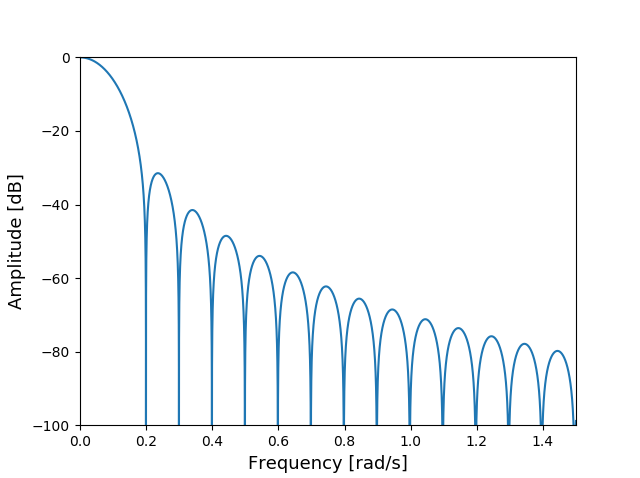
\includegraphics[width=\textwidth]{figures/dbplots/stft_bilag/64/hann.png}
\caption{Hann}
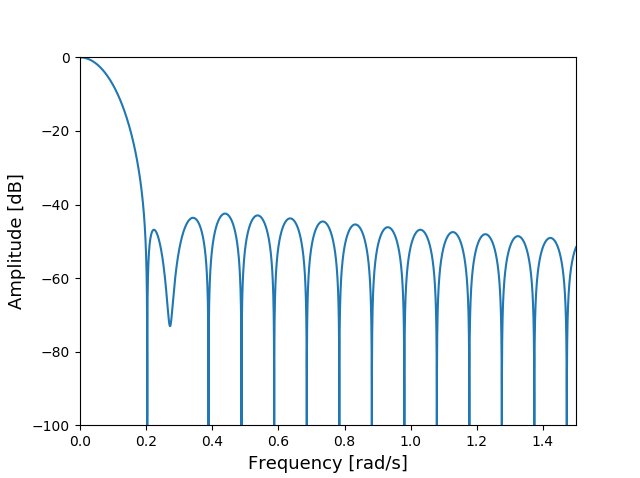
\includegraphics[width=\textwidth]{figures/dbplots/stft_bilag/64/hamming.png}
\caption{Hamming}
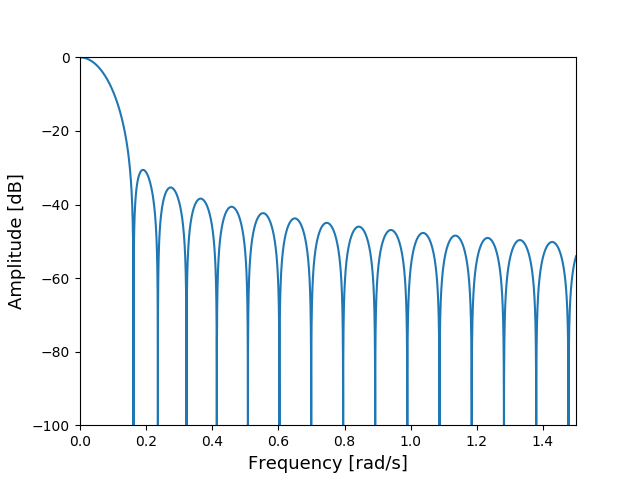
\includegraphics[width=\textwidth]{figures/dbplots/stft_bilag/64/kaiser4.png}
\caption{Kaiser, $\beta=4$}
\end{subfigure}
\centering
\begin{subfigure}{0.49\textwidth}
\centering
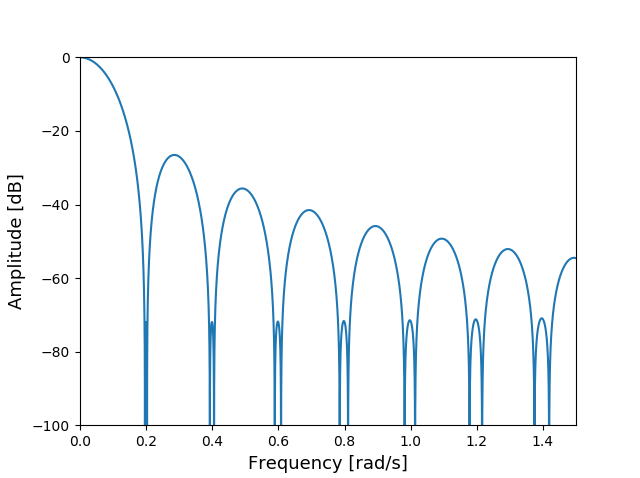
\includegraphics[width=\textwidth]{figures/dbplots/stft_bilag/64/bartlett.png}
\caption{Bartlett}
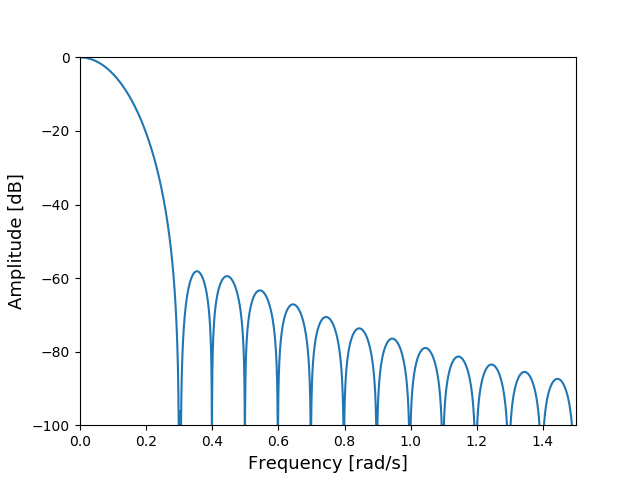
\includegraphics[width=\textwidth]{figures/dbplots/stft_bilag/64/blackman.png}
\caption{Blackman}
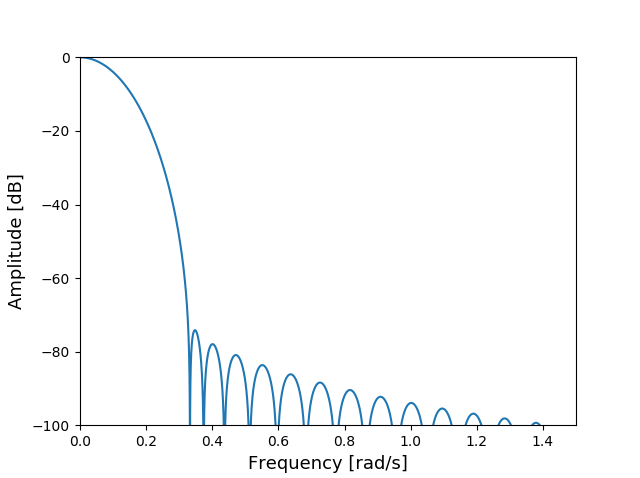
\includegraphics[width=\textwidth]{figures/dbplots/stft_bilag/64/kaiser10.png}
\caption{Kaiser, $\beta=10$}
\end{subfigure}

\caption{Amplitude response of window functions of order $M=64$}
\label{fig:db_plots_64}
\end{figure}

\begin{figure}[H]
\centering

\begin{subfigure}{0.49\textwidth}
\centering
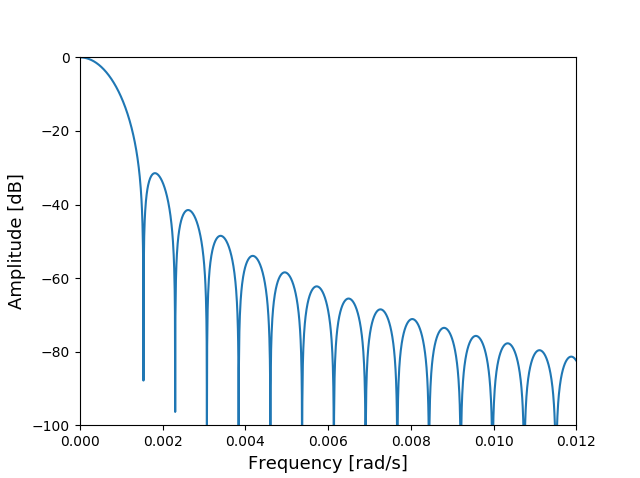
\includegraphics[width=\textwidth]{figures/dbplots/stft_bilag/8192/hann.png}
\caption{Hann}
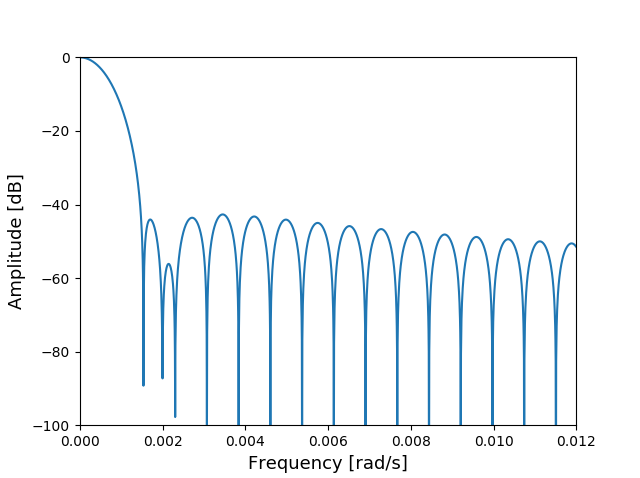
\includegraphics[width=\textwidth]{figures/dbplots/stft_bilag/8192/hamming.png}
\caption{Hamming}
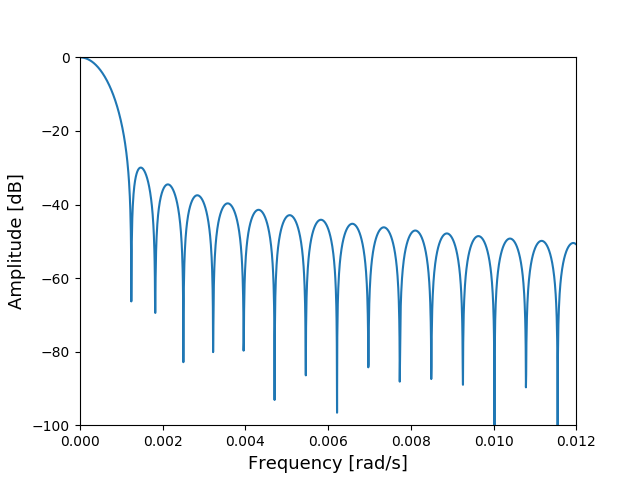
\includegraphics[width=\textwidth]{figures/dbplots/stft_bilag/8192/kaiser4.png}
\caption{Kaiser, $\beta=4$}
\end{subfigure}
\centering
\begin{subfigure}{0.49\textwidth}
\centering
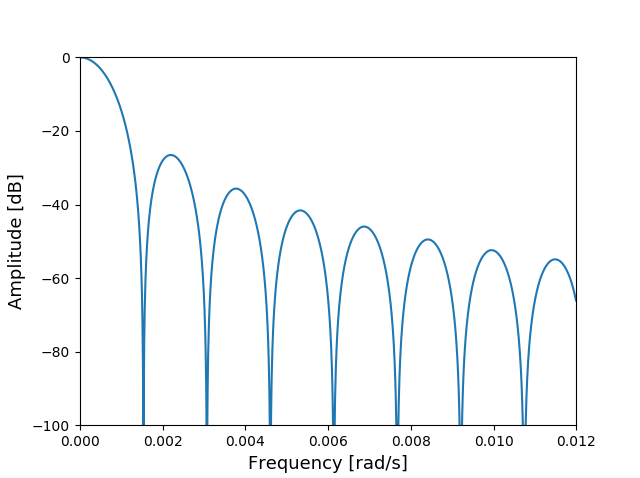
\includegraphics[width=\textwidth]{figures/dbplots/stft_bilag/8192/bartlett.png}
\caption{Bartlett}
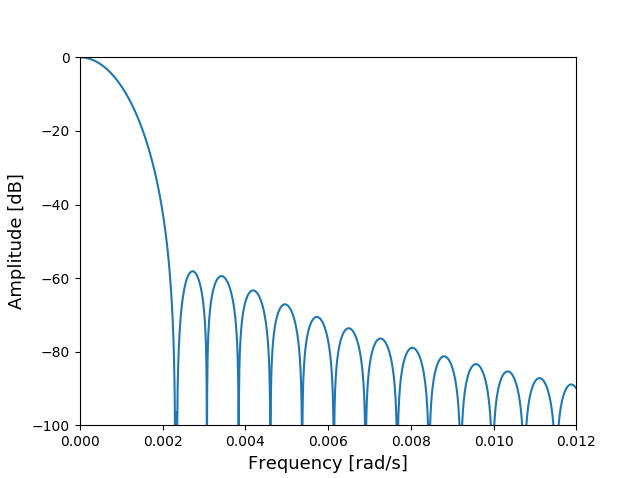
\includegraphics[width=\textwidth]{figures/dbplots/stft_bilag/8192/blackman.png}
\caption{Blackman}
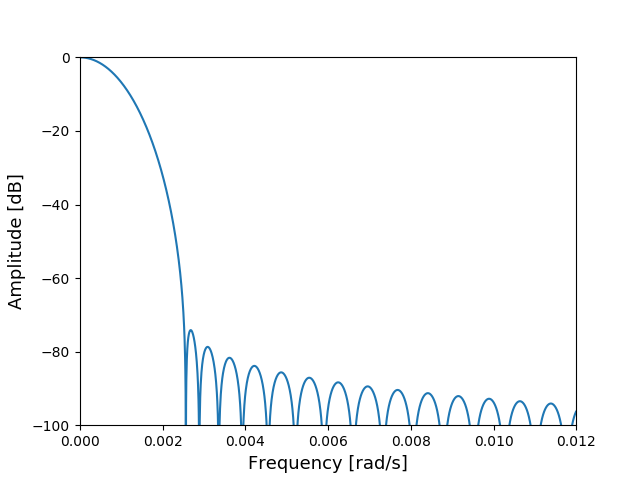
\includegraphics[width=\textwidth]{figures/dbplots/stft_bilag/8192/kaiser10.png}
\caption{Kaiser, $\beta=10$}
\end{subfigure}

\caption{Amplitude response of window functions of order $M=8192$}
\label{fig:db_plots_8192}
\end{figure}




\clearpage
\input{sections/appE/appEwindows_table.tex}

\end{document}